\documentclass[11pt]{article}

\setcounter{tocdepth}{3}
\setcounter{secnumdepth}{3}

\usepackage{comment} % enables the use of multi-line comments (\ifx \fi) 
\usepackage{lipsum} %This package just generates Lorem Ipsum filler text. 
\usepackage[a4paper,margin=1.5cm]{geometry}
\usepackage[utf8]{inputenc}
\usepackage{gensymb}
\usepackage{graphicx}
\usepackage{booktabs}% http://ctan.org/pkg/booktabs
\usepackage{makecell}
\usepackage{tabularx}
\usepackage[table]{xcolor}
\usepackage{array}
\usepackage{wrapfig}
\usepackage{subcaption}
\usepackage{csquotes}
\usepackage{lscape}
\usepackage{afterpage}
\usepackage{geometry}
\usepackage{listingsutf8}
\usepackage{chngcntr}
\usepackage{multicol}
\usepackage{xcolor}
\usepackage{pifont}
\usepackage{outlines}
\usepackage{amsmath}
\usepackage{amssymb}
\usepackage{breqn}
\usepackage{textcomp}
\usepackage{bm}
\usepackage{caption}
\usepackage{enumitem}
\usepackage{hyperref}
\usepackage{mdframed}

\newmdtheoremenv{theorem}{Theorem}

\counterwithin{figure}{section}

\AtBeginDocument{\counterwithin{lstlisting}{section}}

\geometry{a4paper, margin=1in}

\renewcommand*{\thead}[1]{\bfseries #1}
\newcommand{\code}[1]{\texttt{#1}}
\def\doubleunderline#1{\underline{\underline{#1}}}

\newcommand \tabitem{\makebox[1em][r]{\textbullet~}}

\DeclareMathSizes{12}{30}{16}{12}

\definecolor{lightgray}{rgb}{.9,.9,.9}
\definecolor{darkgray}{rgb}{.4,.4,.4}
\definecolor{purple}{rgb}{0.65, 0.12, 0.82}
\definecolor{darkgreen}{rgb}{0.05,0.56,0.06}


\lstset{frame=tlrb,
    language=python,
    captionpos=b,
    aboveskip=3mm,
    belowskip=3mm,
    showstringspaces=false,
    columns=flexible,
    basicstyle={\small\ttfamily},
    numbers=left,
    numberstyle=\tiny\color{gray},
    keywordstyle=\color{blue},
    commentstyle=\color{violet},
    stringstyle=\color{darkgreen},
    breaklines=true,
    breakatwhitespace=true,
    tabsize=3,
    literate=%
    {Ö}{{\"O}}1
    {Ä}{{\"A}}1
    {Ü}{{\"U}}1
    {ß}{{\ss}}1
    {ü}{{\"u}}1
    {ä}{{\"a}}1
    {ö}{{\"o}}1
}


\begin{document}

\title{Machine Learning FS2019\\[0.2em]\normalsize{\url{https://github.com/taneher/HSLU/tree/master/FS19/ML}}}
\author{Alex Neher, Pascal Baumann}
\maketitle

\tableofcontents

\newpage
\graphicspath{{./Pictures/}}

\section{Introduction}

There are two popular definitions of Machine Learning:

\begin{centering}
    \begin{quote}
        \blockquote[Arthur Samuel, IBM, 1959]{Field of study that gives computers the ability to earn without being explicitly programmed}
    \end{quote}

    \begin{quote}
        \blockquote[Tom Mitchell, 1998]{A computer program is said to learn from experience $E$ with respect to some task $T$ and some performance measure $P$, if its performance on $T$, as measured by $P$, improves with experience $E$}
    \end{quote}
\end{centering}

So summarizing these two quotes, it can be said, that machine learning is defined as \textbf{the process in which machines learn something (mostly) on their own}.

\subsection{Disciplines}

There are different disciplines in machine learning:

\begin{description}
    \item[Supervised Learning: ] The algorithm is given \textbf{labeled training data} and learns to \textbf{predict} the \textbf{labels} of yet unseen examples.
    \item[Unsupervised Learning: ] The algorithm is given \textbf{unlabeled data} and \textbf{creates labels by itself} based on the structure of the given data
    \item[Semi-Supervised Learning: ] A \textbf{mixture} of supervised and unsupervised learning. This approach is usually chosen if there is only \textbf{very little labeled test data}
    \item[Reinforcement Learning: ] No data is availabe, but the algorithm is \textbf{being rewarded}. The algorithm searches the ideal behaviour that maximizes its reward (Not subject of this lecture)
\end{description}

These classifications can be subdivided even more:

\begin{figure}[htb!]
    \centering
    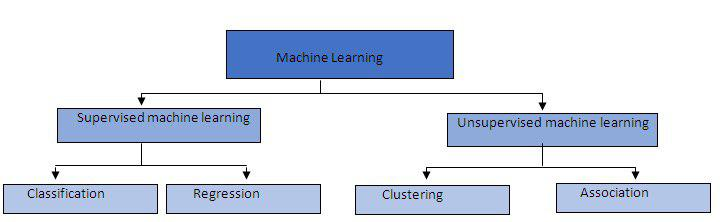
\includegraphics[keepaspectratio=true, width=0.9\textwidth]{disciplines.jpg}
    \caption{Distinction between supervised and unsupervised learning}
    \label{fig:class}
\end{figure}

The main difference between \textbf{classification} and \textbf{regression} is that when using classification, the result is \textbf{categorical}, whereas regression returns \textbf{numerical} results.

\textbf{Clustering} is similar to classificiation. However, while classification algorithms sort the given data into given groups, clustering algorithms determine these groups \textbf{by themself}. This means, you can give a clustering algorithm a seemingly random dataset and the algorithm finds some kind of structure in it.

\newpage

\section{Data Quality}

Data is categorized into \textbf{numerical} and \textbf{categorical} data.

\begin{figure}[htb!]
    \centering
    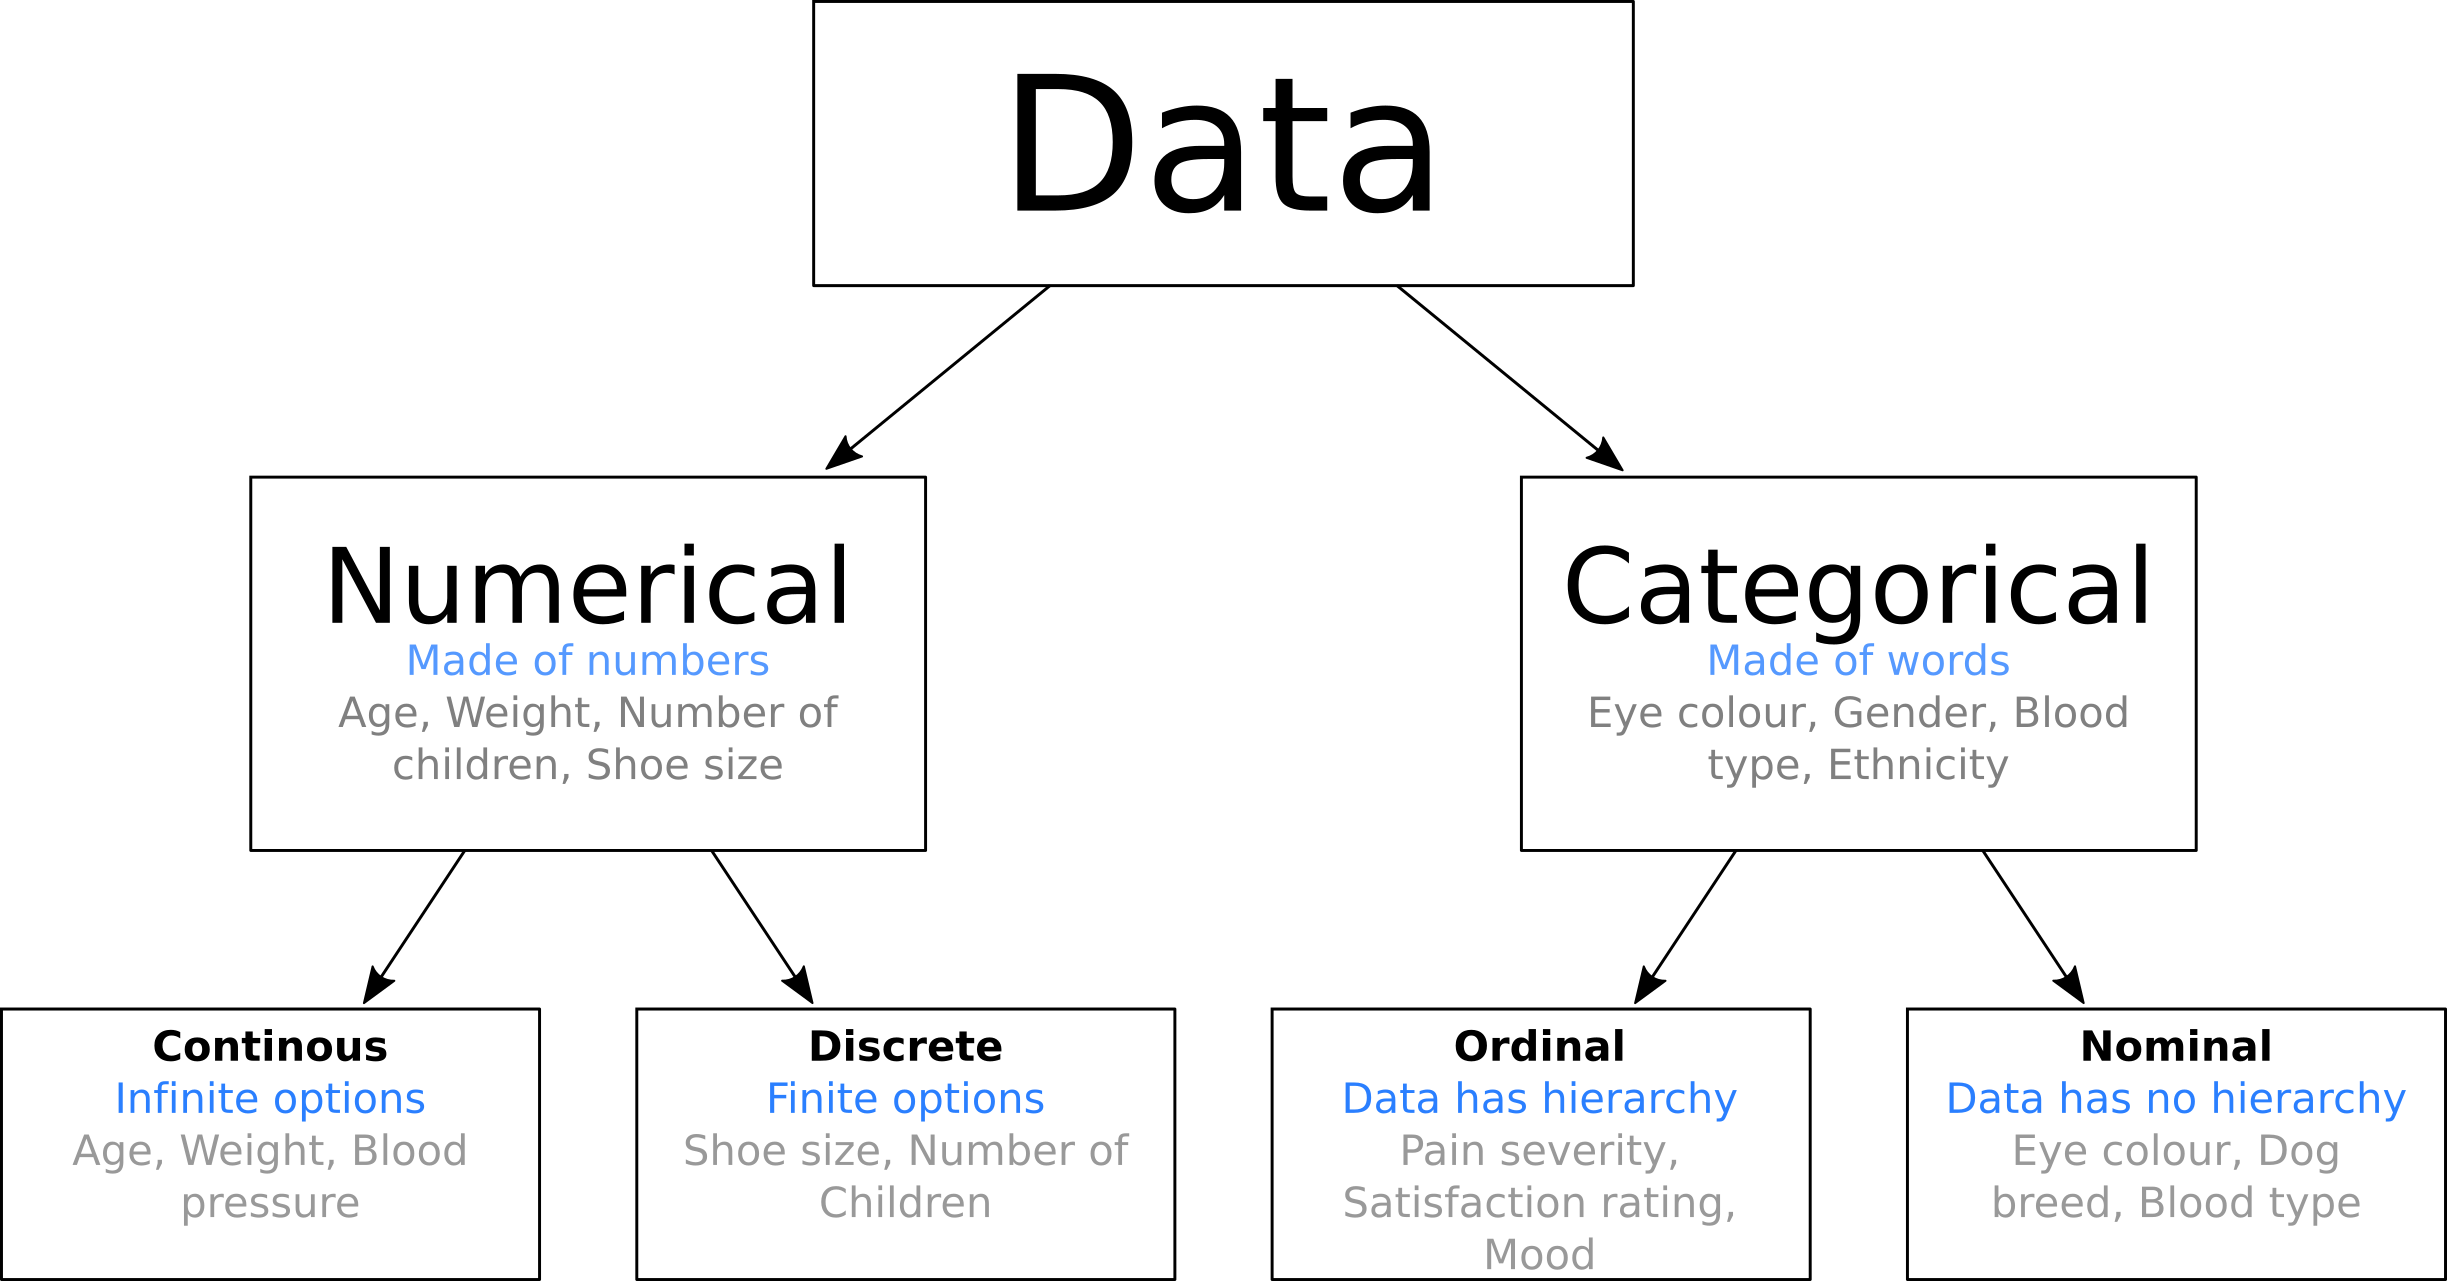
\includegraphics[keepaspectratio=true, width=0.9\textwidth]{data_classification.png}
    \caption{Classification of Data}
    \label{fig:data_classification}
\end{figure}

Before any machine learning can take place, the quality of the given data has to be assessed and in some cases improved. Because every prediction made by machine learning algorithms is shit if the data quality is shit.

There are many reasons why the data quality could be poor:

\begin{itemize}
    \item Ill-designed, inadequate or inconsistent data formats
    \item Programming errors or technical issues (e.g. sensor outage)
    \item Data decay (e.g. outdated e-mail addresses)
    \item Poorly designed data entry forms (e.g. data fields without verification)
    \item Human errors in data export or data pre-processing
    \item Deliberate errors and false information (e.g. due to privacy concerns everybody is called Hans Muster and lives at Musterstrasse 123)
\end{itemize}

\subsection{Data Quality Assessment}

Before even starting to assess the data-quality, it is seldomly a bad idea to \textbf{clean} the data first.

\begin{enumerate}
    \item Identify and remove duplicates
    \item Replace null-values (do not delete them because that might falsify the mean and median of the data)
    \item Make data formats more machine-friendly (so-called \textit{data-wrangling} e.g. store the gender as boolean)
\end{enumerate}

\newpage

If you change anything from the original data set, you should always

\begin{itemize}
    \item Document all the changes
    \item Use a SVN (e.g. git)
    \item Let the data provider know that his data quality is shit (maybe they'll improve in the future)
    \item Investigate the origins of the poor data quality
\end{itemize}

\subsection{Approaches to Data Quality Assessment}

\begin{description}
    \item[Identify data sources and their trustworthiness]
    \item[Interpret statical key figures: ] See following sections
    \item[Visualize selected portions of the data: ] e.g. with Pair Plots (See Abb. \ref{fig:pair_plots} )
    \item[Manually check data ranges] Negative Salaries, People more than 200 years old...
    \item[Validate plausibility of attribute correlation: ] e.g. are mileage and number of seats in a core correlated? Can one of the columns be removed for redundancy?
    \item[Measure data redundancy: ] Can certain columns be removed due to not adding any real value to the data
    \item[Check for anomalies in syntax and semantics: ] Outliers can really distort a dataset and render the whole algorithm useless. Can be prevented by e.g. normalization of the data or removal of the outlier
    \item[Replace NULL Values and remove duplicate values]
\end{description}

There are different ways to cope with NULL variables, but they have to be addressed, as most machine learning algorithms do not play well with them.

\begin{itemize}
    \item Delete all rows with NULL values \\
          Might be the easiest way if you have loads of data
    \item Fill in the missing values manually (e.g. from other sources) \\
          Might be the hardest way if you have loads of data
    \item Fill in a global constant like N/A, UNKNOWN
    \item Use a measure for central tendency \\
          e.g. take the mean if your data is symmetric or take the median if its skewed
    \item Use a measure for central tendency per class \\
          e.g. take different values for healthy and sick people
    \item Use e.g Regression to 'guess' the missing values
\end{itemize}

\begin{figure}[htb!]
    \centering
    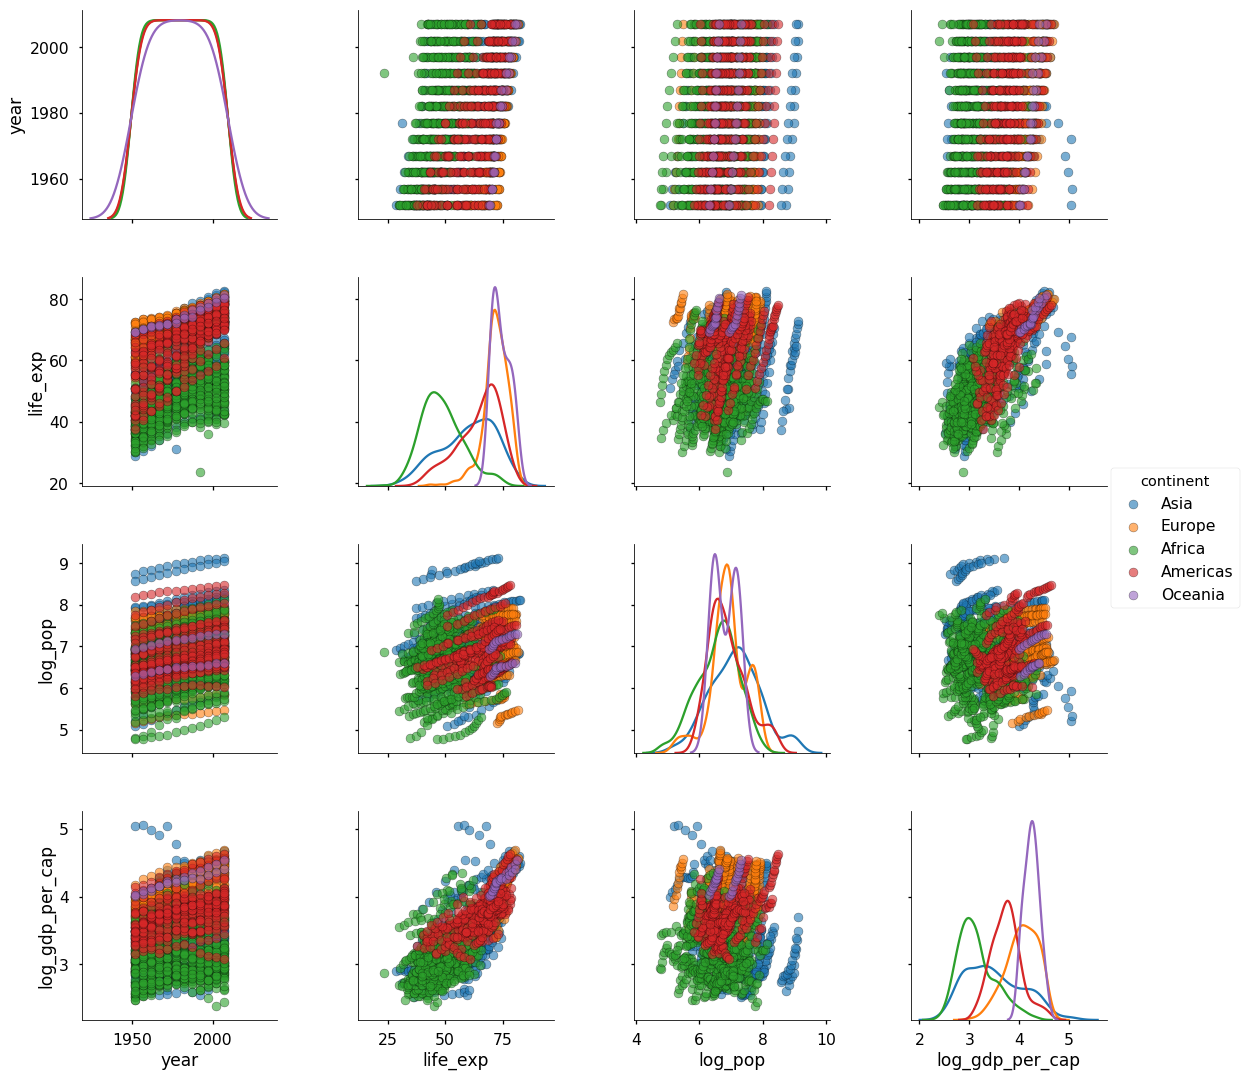
\includegraphics[keepaspectratio=true, width=0.4\textheight]{pair_plots.png}
    \caption{Visualisation of Data with Pair Plots}
    \label{fig:pair_plots}
\end{figure}

\newpage

\subsection{Statistical Key Figures}

These figures can give you a rough overview about the whereabouts of your data-magnitude.

\subsubsection{Central Tendency}

\textbf{Mean} \\

This is the averge in a set of numeric data. You add all data and divide it by the number of data points

\begin{equation}
    \mu_{x}=\frac{1}{n} \sum^{n}_{i=1} x_{i}
\end{equation}

\vspace{10px}

\noindent \textbf{Mode} \\

This is the value that occurs the most in a given set of data

\vspace{10px}

\noindent \textbf{Median} \\

This is the middlemost value of a sorted set of data. In contrast to the Mean, the Median can give information concerning the distribution of the data.

Given a dataset of $1, 2, 3, 4, 5$, the median and mean are both $3$. However, if we have $1, 2, 3, 1000, 10000$, the mean is $2201.2$ whereas the mean is still $3$

\newpage

\subsubsection{Skewdness}

All of these values can give information concerning the datas \textbf{skewness}

\begin{figure}[htb!]
    \centering
    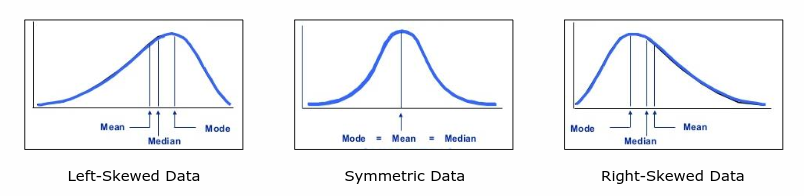
\includegraphics[keepaspectratio=true, width=0.9\textwidth]{skewness.png}
    \caption{Skewness of data}
    \label{fig:skewness}
\end{figure}

\noindent
$Mean - Mode > 0 \rightarrow$ Negative skewness / Left-skewed data \\
$Mean - Mode = 0 \rightarrow$ Symmetric Data \\
$Mean - Mode > 0 \rightarrow$ Positive skewness / Right-skewed data

\vspace{10px}

\subsubsection{Quartile \& Interquartile Range (IQR)}

The three quartiles divide your data into four equal-sized, cnsecutive subsets.

To calculate $Q1$, take the median of your data and then again the madian of the left half of the data.

\begin{figure}[htb!]
    \centering
    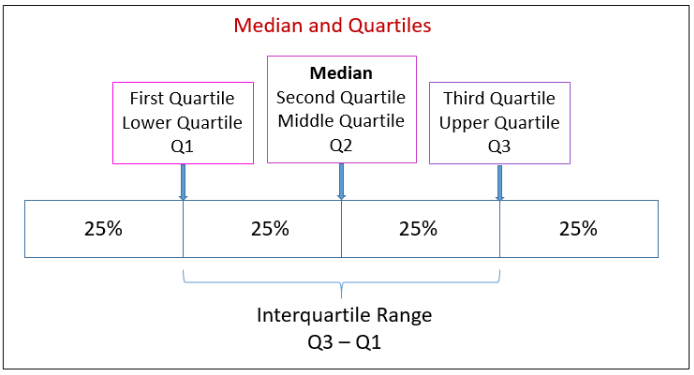
\includegraphics[keepaspectratio=true, width=0.9\textwidth]{iqr.png}
    \caption{Quartiles of a dataset}
    \label{fig:iqr}
\end{figure}

\newpage

\subsubsection{Five Number Summary}

With this method, you can get a pretty good overview of your data. The \textbf{Five Number Summary} of a dataset consists of:

\begin{itemize}
    \item Median Q2
    \item Quartiles Q1 and Q2
    \item Smallest individual Value
    \item Largest individual Value
\end{itemize}

\begin{minipage}{0.45\textwidth}
    \begin{lstlisting}[caption={Five Number Summary in Python}]
    import numpy as np
    import panas as pd

    s = pd.Series(np.random.rand(100))
    s.describe()
    \end{lstlisting}
\end{minipage}\hfill
\begin{minipage}{0.45\textwidth}
    \begin{lstlisting}[caption={Output}]
    mean       0.524559
    std        0.285565
    min        0.003933
    25%        0.298367
    50%        0.530632
    75%        0.765907
    max        0.993293
    dtype: float64
    \end{lstlisting}
\end{minipage}

\subsubsection{Boxplot}

\begin{wrapfigure}[14]{R}{0.5\textwidth}
    \centering
    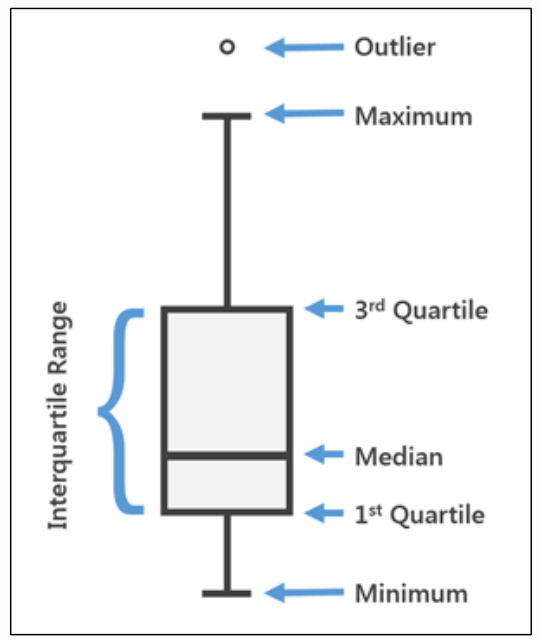
\includegraphics[keepaspectratio=true,height=14\baselineskip]{boxplot.png}
    \caption{Boxplot}
    \label{fig:boxplot}
\end{wrapfigure}

This plot is a \textbf{visual representation of the five number summary} and can also give information on potential outliers.

Values $1.5 \cdot IQR$ above the 3rd or below the 1st Quartile can be considered outliers and are displayed with small circles.

\subsubsection{Variance}
The variance shows \textbf{how much the values are spread on average}. This is measured by squaring the sum of all deviations from the mean

\begin{equation}
    \frac{1}{1-n} \sum^{n}_{i=1}(x_{i} - \mu x)^2
\end{equation}

The standard deviation $\sigma$ is calculated as $\sqrt{variance}$

\newpage

\subsubsection{Covariance}
The covariance is used to determine whether two variables are \textbf{connected} to each other.

If both variables are on the same side of the mean, the variance is \textbf{positive}, the variables are probably connected. Meaning if the value of one variable is rising, the other one will most likely rise as well.

If one is above and one is below the mean, the variance is \textbf{negative}, the variables are most likely \textbf{inversely connected} to each other. Meaning if the value of one variable is rising, the other is most likely falling.

If the variables are \textbf{independent} from each other, the covariance is zero, as they both cancel each other out.

\begin{equation}
    Cov(x,y) = \frac{1}{1-n} \sum^{n}_{i=1}(x_{i} - \mu x)(y_{i} - \mu y)
\end{equation}

The \textbf{covariance matrix} shows the covariance from all $X$ with all $Y$. As $Cov(x,x) = Var(x)$, the covariance matrix has the variance of $X$ in its diagonal


\subsubsection{Pearson Correlation} \label{sec:pearson}
Both the covariance and the variance are connected to the scale of the dataset, so the covariance of $X=[1,2,3,4,5] / Y=[6,7,8,9,10]$ is 2.5, whereas the covariance of $X=[1000,2000,3000,4000,5000] / Y=[6000,7000,8000,9000,10000]$ is 2'500'000'000. However, the Perason Correlation is 1 in both examples.

\begin{equation}
    \rho(X,Y)=\frac{Cov(X,Y)}{\sigma_{x} \sigma_{y}} =
    \frac{\frac{1}{1-n} \sum^{n}_{i=1}(x_{i} - \mu x)(y_{i} - \mu y)}{\sqrt{\frac{1}{1-n} \sum^{n}_{i=1}(x_{i} - \mu x)^2} \cdot \sqrt{\frac{1}{1-n} \sum^{n}_{i=1}(y_{i} - \mu y)^2}}
\end{equation}
The Pearson Correlation is always between 1 and -1.

\noindent 1 means the data is perfectly correlated, whereas -1 means that the data is perfectly incorrelated

\subsection{Normalization}
It is immensely important that all data is normalized before we run a machine learning algorithm over it. Considering the data in figure \ref{fig:vector_space_modefig}, 'Mileage' and 'Price' are in a completely different scale. If the mileage of the first shown car goes up 500 miles, it's not really a big deal. However, a price increase by 500 would double the car's price.

Such differently scaled data can (and will) falsify the result of every machine learning algorithm you could find. Therefore, \textbf{normalization is really important}.

\vspace{10px}

\noindent There are two popular normalization approaches: The Min-Max and the Z-Score normalization.

\newpage

\noindent \textbf{Min-Max normalization}

\noindent All data is condensed to a value between 0 and 1. The smallest value becomes 0 and the largest one becomes 1.

\begin{equation}
    x \rightarrow \frac{x - min_{x}}{max_{x}-min_{x}}
\end{equation}

\noindent \textbf{Z-Score Normalization}

\noindent The dataset is transformed in such a way, that the mean becomes 0 (so-called \textit{mean-centering}) and the standard deviation is 1

\begin{equation}
    x \rightarrow \frac{x - \mu_{x}}{\sigma_{x}}
\end{equation}

\section{Geometry of Data}

\subsection{Feature Engineering}

Sometimes, data has to be modified to be better accessible/processable for machine learning algorithms. These algorithmus can work the best with simple numbers, so that's the data we should be striving for:

\begin{figure}[htb!]
    \centering
    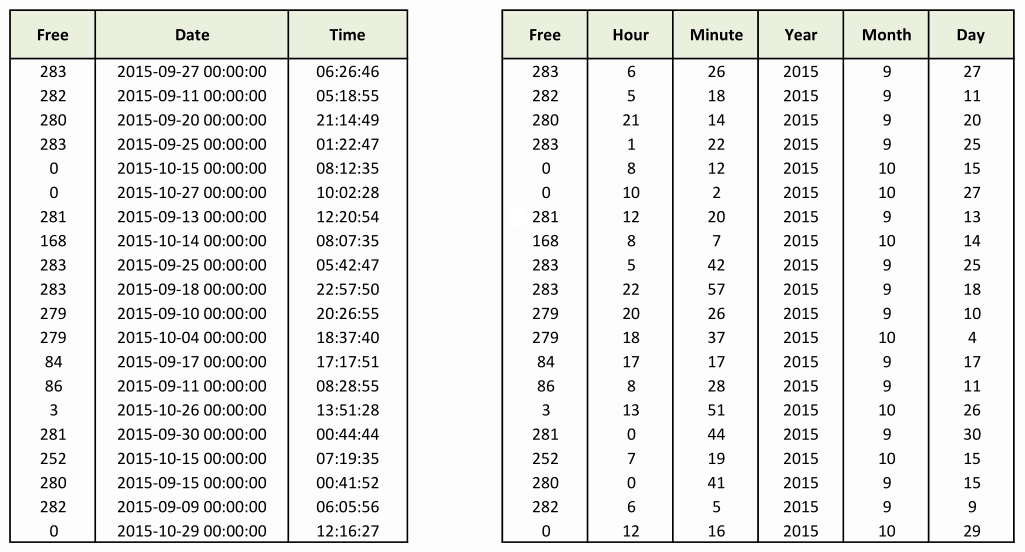
\includegraphics[keepaspectratio=true, width=\linewidth]{feature_engineering.png}
    \caption{Turn 'complicated' data into easier data for better results}
    \label{fig:feature_engineering}
\end{figure}

\subsection{Vector Space Model}

As described before, machine learning algorithms work best with \textbf{numeric} data. However, the real world isn't that easy and mostly throws categorical data at you. Therefore, you have to convert categorical data to numerical data.

\begin{figure}[htb!]
    \centering
    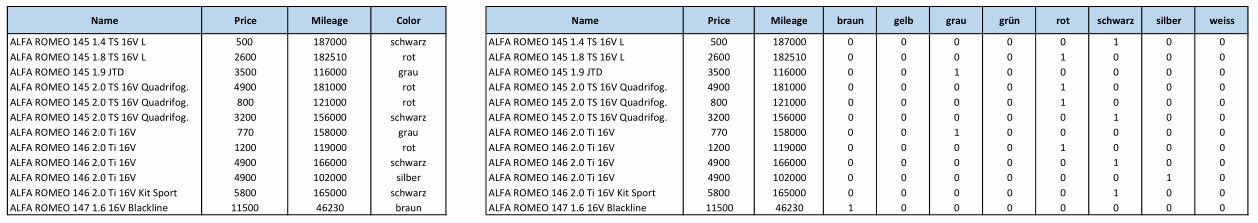
\includegraphics[keepaspectratio=true, width=\linewidth]{vector_space_model.png}
    \caption{Turn categorical data into numerical data with the vector space model}
    \label{fig:vector_space_modefig}
\end{figure}

This transformed data can also be visualized in a coordinate system and we can do math with it.

\begin{figure}[htb!]
    \centering
    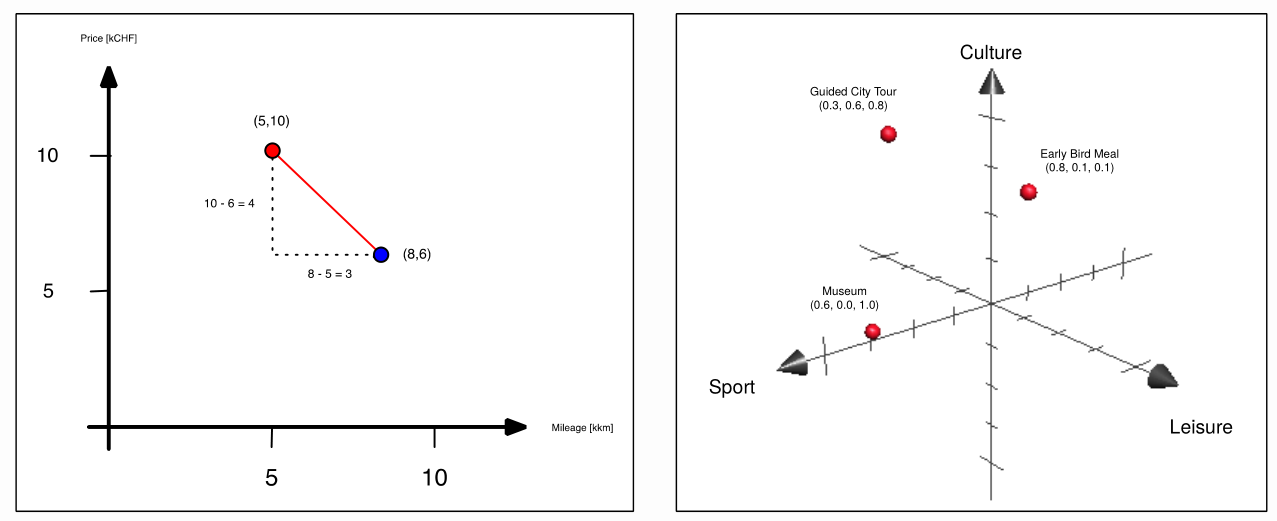
\includegraphics[keepaspectratio=true, width=\linewidth]{geometric_interpretation.png}
    \caption{Transformed into vector space, data points can be interpreted as geometric points}
    \label{fig:geometric_intepretation}
\end{figure}

\newpage

\subsection{Similarity of Data}

The math we want to do is not even overly complicated: We just want to measure the distance between different points. Because \textbf{the smaller the distance between two points, the more similar they are}.

\subsubsection{Euclidean Distance}

The distance between two points is most easily calculated using the \textbf{euclidean distance}:

\begin{equation}
    dist(X,Y)= \sqrt{\sum^{n}_{i=1}(x_{i}-y{i})^2}
\end{equation}

So the distance between the points $(5/10)$ and $(8/6)$ can be calculated as

\begin{align}
    \sqrt{(5-8)^2 + (10-6)^2} \\
    \sqrt{-3^2 + 4^2}         \\
    \sqrt{9+16}               \\
    \sqrt{25} = 5
\end{align}

\newpage

\subsubsection{Cosine Similarity}

\begin{wrapfigure}[14]{R}{0.5\textwidth}
    \centering
    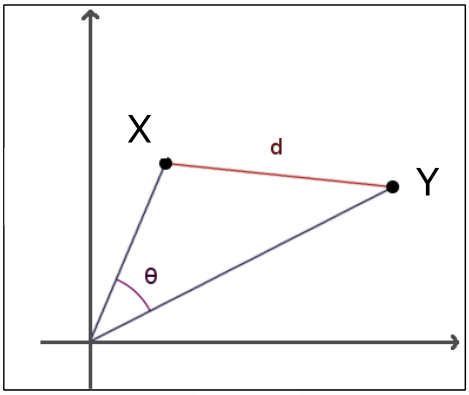
\includegraphics[keepaspectratio=true,height=14\baselineskip]{cosine_similarity.png}
    \caption{Cosine Similarity}
    \label{fig:cosine_similarity}
\end{wrapfigure}

If you want to to compare two points that appear to be on a line (Pearson Correlation close to 1), but the euclidean distance is high, then the cosine similarity is probably pretty low.

The cosine similarity looks at the \textbf{angle} between point A and point B. However, it does also take the euclidean distance into consideration.

\vspace{10px}

The cosine similarity is essentially just the scalar product of the two points.

\vspace{10px}

\begin{equation} \label{eq:sim}
    sim(X,Y) = \frac{\sum^{n}_{i=i}{x_{i} y_{i}}}{\sqrt{\sum^{n}_{i=i}{x_{i}}^2\sqrt{\sum^{n}_{i=i}{y_{i}}^2}}}
\end{equation}
\begin{equation}
    dist(X,Y) = 1 - sim(X,Y)
\end{equation}

\subsubsection{Levenshtein / Edit Distance for Strings}

Count the minimal number of changes necessary to turn one string into another:
\begin{itemize}
    \item count +1 when deleting a character [d]
    \item count +1 when adding a character [a]
    \item count +2 when changing a character [c]
\end{itemize}

\begin{figure}[htb!]
    \centering
    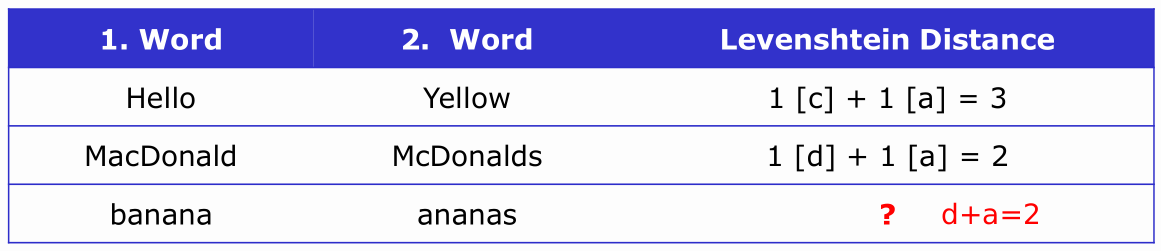
\includegraphics[keepaspectratio=true, width=\linewidth]{levenshtein.png}
    \caption{Examples for Levenshtein Distance}
    \label{fig:levenshtein}
\end{figure}

\newpage

\section{Supervised Machine Learning}

\subsection{Regression and classification algorithms}

\begin{multicols}{2}
    \textbf{Regression}
    \begin{itemize}
        \item Linear Regression
        \item Polynomial Regression
        \item k-NN Regression
        \item Support Vector Regression
        \item Neural Networks
        \item Regression Trees
    \end{itemize}
    \columnbreak
    \textbf{Classification}
    \begin{itemize}
        \item Logistic Regression
        \item Naïve Bayes
        \item k-NN
        \item Support Vector Machines
        \item Neural Networks
        \item Decision Trees
    \end{itemize}
\end{multicols}

\subsection{Decision Boundaries}

\begin{figure}[htb!]
    \centering
    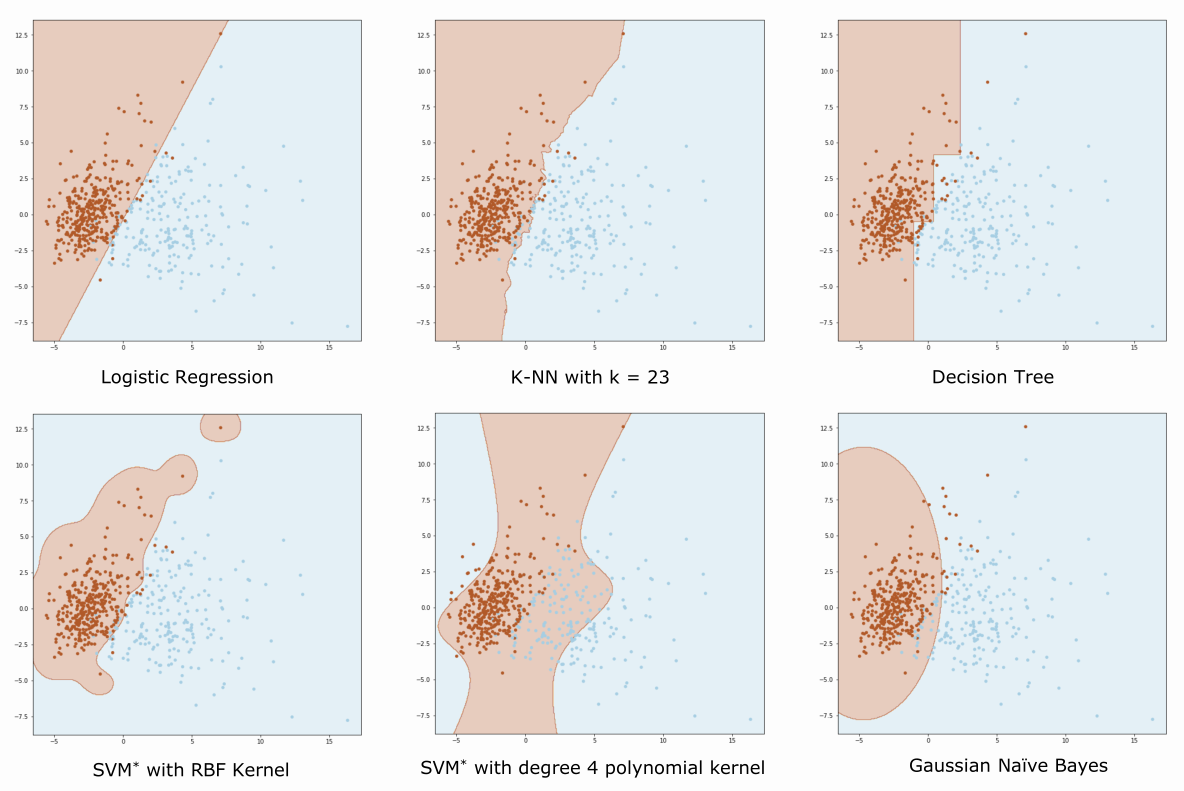
\includegraphics[keepaspectratio=true, width=\linewidth]{decision_boundaries.png}
    \caption{Decision Boundaries for different classification approaches}
    \label{fig:decision_boundaries}
\end{figure}

Classifications usually end in somithing like Figure \ref{fig:decision_boundaries}. The example shows a classification whether a tumor is benign or cancerous. Brown means cancerous and blue means benign. Even though the data points are the same in all pictures, different approaches yield different results.

The goal of a 'good' classification-algorithm is to produce as few false-positive (algorithm says is cancer, but is actually not) and false-negatives (algorithm says its benign but is actually cancerous) as possible.

\subsubsection{Kernel-Trick}
The data in Fig. \ref{fig:decision_boundaries} is still theoretically linearly separable. But in case it is not, you could use the so-called 'kernel-trick', where you simply add a dimension and change your point of view (see Fig. \ref{fig:kernel_trick})

\begin{figure}[htb!]
    \centering
    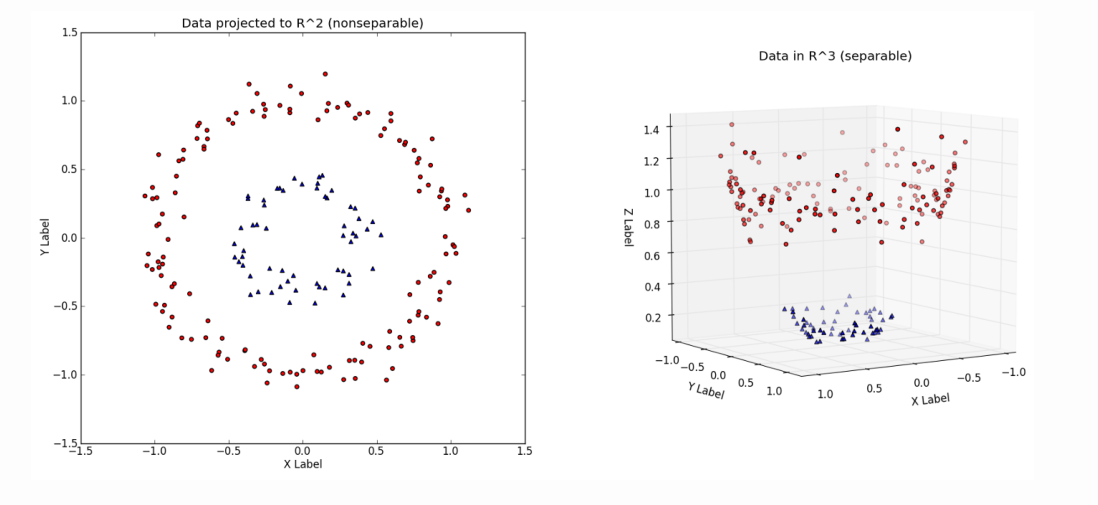
\includegraphics[keepaspectratio=true,height=11\baselineskip]{kernel_trick.png}
    \caption{Kernel Trick to linearly separate data that is not linearly separable}
    \label{fig:kernel_trick}
\end{figure}

\subsection{k-Nearest-Neighbor}

\begin{minipage}{0.55\textwidth}
    \begin{lstlisting}
    from sklearn.neighbors import KNeighborsClassifier

    knn = KNeighborsClassifier(n_neighbors=3)
    knn.fit(X_train, y_train)
    y_pred = knn.predict(X_test)
    acc = accuracy_score(y_test, y_pred)

    print("Test Set Accuracy for k=3" + ": (:.2f)".format(acc))
    \end{lstlisting}
\end{minipage}\hfill
\begin{minipage}{0.40\textwidth}
    \centering
    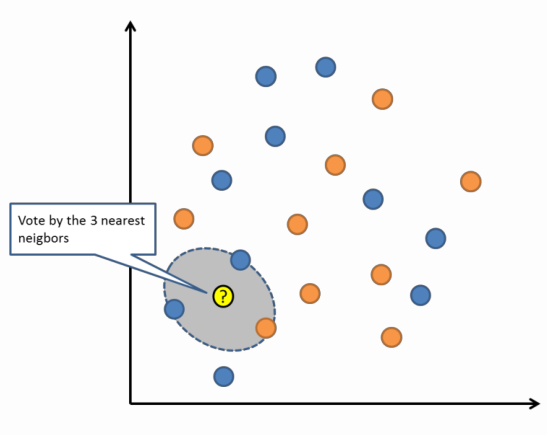
\includegraphics[keepaspectratio=true, width=\textwidth]{knn.png}
\end{minipage}

\vspace{10px}

\begin{wrapfigure}[15]{L}{0.5\textwidth}
    \centering
    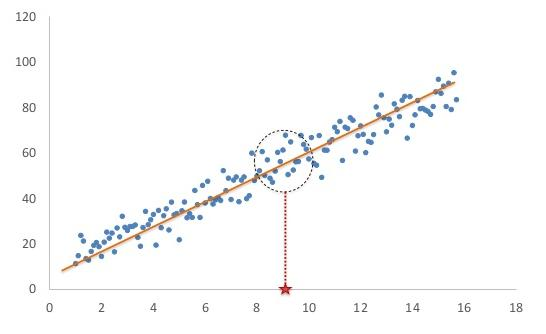
\includegraphics[keepaspectratio=true,height=12\baselineskip]{k-nn-regression.jpg}
    \caption{Regression with k-NN}
    \label{fig:knn-regression}
\end{wrapfigure}

The k-neeares-Neighbor algorithm assigns the label of its nearest datapoint to the sample datapoint. If \code{n\_neighbors} is $>1$, it assigns the label of the most neighbours (via majority voting).

\vspace{10px}

Even though the K-NN algorithm is pretty slow compared to other algorithms, it is often a good choice if you only have a limited amount of data, because other, more performant algorithms usually require a lot more data to get decent predictions.

Usually, k-NN treats all neighbors as equals. However, you could assign a weight to each datapoint. This weight depends on the distance $d$ from the sample point. This is especially useful if you want to use k-NN to e.g. form a regression line.

You can use k-NN for regression by simply assigning the mean of all $k$ neighbors as label to the sample data.

\subsection{Training- and Testdata}
If you use the same data to train and test your algorithm, it might occur that the algorithm is 'memorizing' the data and gives you brilliant results. However, if you release it into the wild, where it encounters different data, it will perform really poorly. This is called \textbf{overfitting}

To counter overfitting, you usually split your data into \textbf{trainingdata} and \textbf{testdata}. You train the algorithm with the training data and test it with the testdata (who would've thought...).

\begin{figure}[htb!]
    \centering
    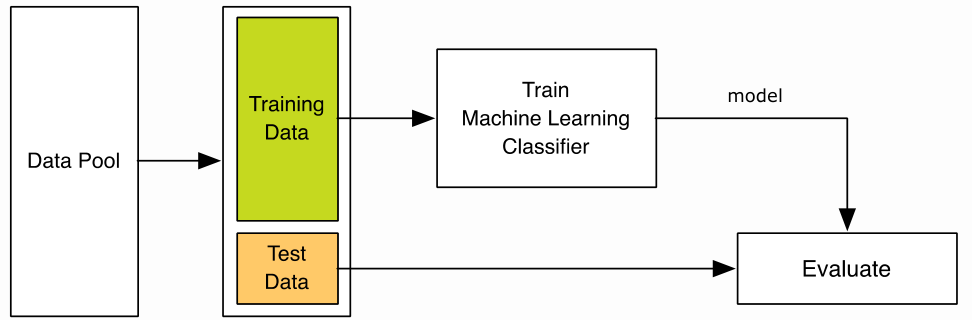
\includegraphics[keepaspectratio=true,width=0.9\textwidth]{training_testdata.png}
    \caption{Split your data into training- and testdata}
    \label{fig:training_testdata}
\end{figure}

\textbf{training} means that you tweak the parameters of the algorithm to minimize the cost function.

\textbf{testing} means that you test the performance of the algorithm with those tweaked parameters on \textit{yet unseen data}. If the algorithm has already seen the data, you might run into overfitting problems.

\vspace{10px}

If you need to tweak your hyperparameters a lot (e.g. the 'k' in k-NN), you should probably use a more complex evaluation workflow. Because if you keep tweaking the hyperparameters and then testing them with the same data, you'll end up with the very same overfitting problem that I explained earlier (and will therefore probably get fired and have to live on the street).

\vspace{10px}

Therefore, it is recommended that you add \textbf{validation data} to your workflow. You train your model with the training data, validate the results with the validatin data, and if the result is satisfactory, you can test it on entirely different test data.

\begin{figure}[htb!]
    \centering
    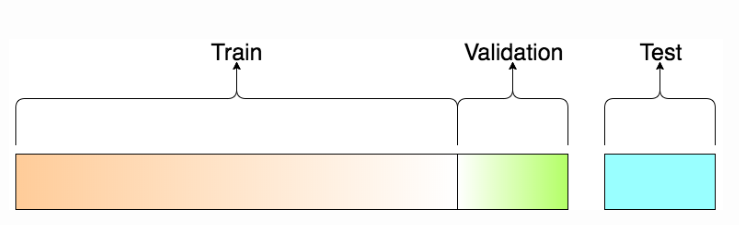
\includegraphics[keepaspectratio=true,width=0.9\textwidth]{validation_data.png}
    \caption{Add validation data to the mix}
    \label{fig:validation_data}
\end{figure}

This method requires quite a lot of data. If you do not have the required amount of data, you could for example use \textbf{cross validation}. You still split your data into training- and testdata and then use a different 'slice' of your training data to validate the hyperparameter.

\begin{figure}[htb!]
    \centering
    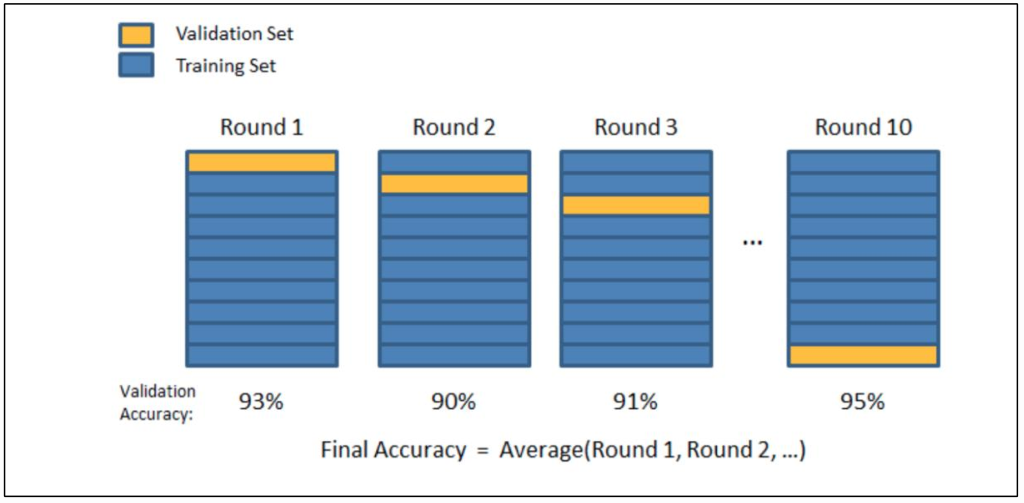
\includegraphics[keepaspectratio=true,width=0.9\textwidth]{cross_validation.png}
    \caption{10-fold cross validation}
    \label{fig:cross_validation}
\end{figure}

\subsection{Measuring the performance of classification}

To verify that your tweaked parameters are indeed within the margin that is acceptable, you need to do some quality assuranc first.

\subsubsection{Confusion Matrix}

\begin{minipage}{0.45\textwidth}
    \begin{tabular}{|p{1.5cm}|p{1.5cm}|p{1.5cm}|}
        \hline
        \thead{n=165} & Predicted YES & Predicted NO \\
        \hline
        Actual No     & 50            & 10           \\
        \hline
        Actual YES    & 5             & 100          \\
        \hline
    \end{tabular}
\end{minipage}\hfill
\begin{minipage}{0.55\textwidth}
    \begin{description}
        \item[True Positive: ] Predicted Yes, Actual Yes
        \item[True Negative: ] Predicted No, Actual No
        \item[False Positive: ] Predicted Yes, Actual No
        \item[False Negative: ] Predicted No, Actual Yes
    \end{description}
\end{minipage}

\vspace{10px}

The confusion matrix shows, how many true/false positives and true/false negatives the algorithm produced.

With these values, one can calculate the algorithms \textbf{Accuracy} and \textbf{Error Rate}

\subsubsection{Accuracy and Error Rate}

\begin{equation}
    Accuracy = \frac{True\ Positive + True\ Negative}{Total}
\end{equation}
\vspace{10px}
\begin{equation}
    Error\ Rate = \frac{False\ Positive + False\ Negative}{Total} = 1 - Accuracy
\end{equation}

\vspace{10px}

In our case the Accuracy would be $\frac{50+100}{50+100+5+10} = \frac{150}{165} = 0.91 = 91\%$ and the error rate therefore 9\%

\newpage

\subsubsection{Sensitivity}

Accuracy works great on balanced data, but it's not reliable on inbalanced data because Accuracy only checks how many times the classifier was right.

If there were 5000 NO instances and 20 YES instances, a classifier that only returns NO would have an accuracy of over 99\%.

\vspace{10px}

\noindent The \textbf{Sensitivity} (also called 'Recall') counts how many true positives there are.

\begin{equation}
    Sensitivity = \frac{True\ Positive}{Actual\ YES} = \frac{True\ Positive}{True\ Positive + False\ Negative}
\end{equation}

\vspace{10px}

In our confusion matrix from earlier, the Sensitivity would be $\frac{100}{100 + 5} = \frac{100}{105} = 0.95 = 95\%$

\subsubsection{Sepcificity}
This is the inverse of the Sensitivity. It counts how many NO the algorithm correctly predicted.o

\begin{equation}
    Specificity= \frac{True\ Negative}{Actual\ NO} = \frac{True\ Negative}{True\ Negative + False\ Positive}
\end{equation}

\vspace{10px}

In our confusion matrix from earlier, the Specificity would be $\frac{50}{50+ 10} = \frac{50}{60} = 0.83 = 83\%$

\subsubsection{Precision}
Both of the preceding measures relied on the true negative. However, what would you do if you could not count the True Negatives? You use \textbf{Precision}. Precision shows how many times the algorithm is correct if it predicts YES.

\begin{equation}
    Precision = \frac{True\ Positive}{Predicted\ YES} = \frac{True\ Positive}{True\ Positive + False\ Positive}
\end{equation}

\vspace{10px}

In our confusion matrix from earlier, the Precision would be $\frac{100}{100+ 10} = \frac{100}{110} = 0.91 = 91\%$

\subsubsection{F1 Score}

The F1 score is the harmonic mean between precision and recall/sensitivity

\begin{equation}
    F1 = \frac{2 \cdot Precision \cdot Sensitivity}{Precision + Sensitivity}
\end{equation}

In our confusion matrix from earlier, the Precision would be $\frac{2 \cdot 0.91 \cdot 0.95}{0.91 + 0.95} = \frac{1.73}{1.86} = 0.93 = 93\%$

\vspace{10px}

Due to the fact that the F1 score does not take True Negatives into account, it tends to be strongly biased towards the worse score.

However, it is still one of the best methods to solve a classification problem with skewed data.


\subsection{Measuring the performance of regression}

\begin{figure}[htb]
    \centering
    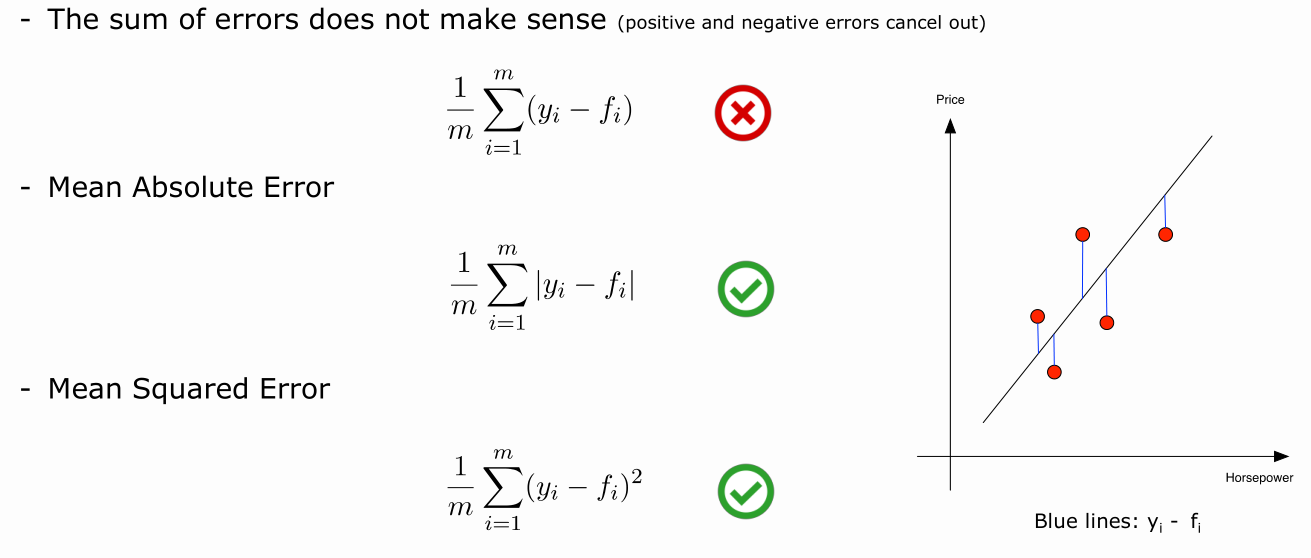
\includegraphics[keepaspectratio=true, width=\linewidth]{regression_error.png}
    \label{fig:regression_error}
\end{figure}

\subsubsection{Coefficient of Determination} \label{sec:r_squared}

\begin{equation}
    R^2 = 1- \frac{\frac{1}{m} \sum^{m}_{i=1}(y_{i} - f_{i})^2}{\frac{1}{m} \sum^{m}_{i=1}(y_{i} - \bar{y})^2} =1 - \frac{\sum^{m}_{i=1}(y_{i} - f_{i})^2}{\sum^{m}_{i=1}(y_{i} - \bar{y})^2}
\end{equation}

$R^2$ is a staticstical measure of how well the predictions approximate the real data points.
The top is the sum of squared errors (how much does the prediction deviate from the actual value) and the botom is the deviation of the mean.

$R^3 = 1$ is a perfect prediction-line

$R^3 = 0.53$ means that 53\% of the of the predictions are correct and can be explained by the model.

\newpage

\section{Gradient Descent}
The problem with Linear Regression is, that it does not scale well. For problems like these we can use Gradient Descent. The gradient (denoted with the Nabla Operator $\nabla$) uses the properties of partial derivatives, which compute the slope in regards to an axis in a point $a,b$.

\begin{figure}[tbh!]
    \centering
    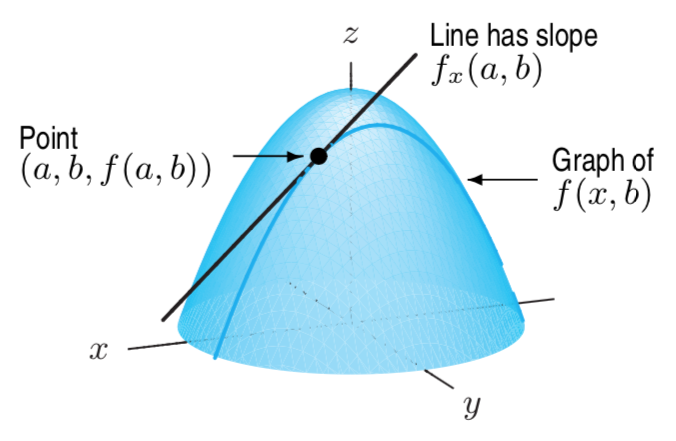
\includegraphics[keepaspectratio=true, width=0.8\linewidth]{Pictures/PartialDerivative}
    \caption{Partial derivative in regards to the x-axis in the point a,b (\textcopyright J. Bürgler, 2019)}
    \label{fig:partialderivative}
\end{figure}

The gradient $\nabla f$ of the scalar function $f: \mathbb{R}^2 \rightarrow \mathbb{R}, (x,y) \mapsto f(x,y) = z$ is a vector, whose components are partial derivatives of $f$.

\begin{equation}
\nabla f(x,y) =
\begin{bmatrix}
\frac{\delta f}{\delta x}(x,y) \\
\frac{\delta f}{\delta z}(x,y)
\end{bmatrix}
=
\begin{bmatrix}
f_x (x,y) \\
f_y (x,y)
\end{bmatrix}
\end{equation}

\subsubsection{Example of a gradient}

Calculate the gradient of the function $f(x,y) = (3x+2y)^2$ in general and in the point $(1,2)$.

\begin{align*}
\nabla f(x,y) & = \begin{bmatrix}
6(3x + 2y) \\
4(3x + 2y)
\end{bmatrix} \\
\nabla f(1,2) & = \begin{bmatrix}
42 \\
28
\end{bmatrix}
\end{align*}

\subsection{Properties of the gradient}
\begin{itemize}
    \item The Gradient of a function f is a vector consisting of the partial derivatives of f with respect to all of its variables
    \item It points to the direction of maximal increase
    \item The negative Gradient points to the direction of maximal decrease
    \item The Gradient being a null-vector indicates a local extrema
    \item The Gradient is perpendicular to the contour lines of that function
\end{itemize}

\subsection{Gradient descent}
To find a local minima of a function $f$ we follow the direction of the steepest descent, and thus the negative Gradient. As the Gradient is constantly changing, we have to take small steps.

\subsubsection{Batch Gradient Descent}
Elevating the strengths of vectors we can Gradient Descent along all columns of our data. For this we want to minimize the cost function
\begin{equation}
J(\theta) = \frac{1}{2n}\sum_{i=1}^{n}(h(bm{\theta},\textbf{x}^{(i)})-y^{(i)})^2
\end{equation}

where $h(\bm{\theta},\textbf{x}^{(i)})$ is

\begin{equation}
h(\bm{\theta},\bm{x}^{(i)}) = \bm{x}^{(i)}\bm{\theta} = \theta_0 + \theta_1 x^{(i)}_1 + \theta_2 x^{(i)}_2 + \cdots + \theta_m x^{(i)}_m
\end{equation}

And calculate the next iteration with the learning rate $\alpha$ (usually $0\leq\alpha\leq0.1$)

\begin{equation}
\bm{\theta}_{k+1} = \bm{\theta}_{k} -\alpha\nabla J(\bm{\theta}_k)
\end{equation}

It can be shown that this yields

\begin{equation}
\bm{\theta}_{k+1} = \bm{\theta}_{k} -\alpha\frac{1}{n}(h(\bm{\theta},\bm{x}^{(i)})-y^{(i)})\cdot\bm{x}^{(i)}
\end{equation}

\subsection{Stochastic Gradient Descent}
In Batch Gradient Descent the update to the parameter vector $\bm{\theta}$ is done all at once using the whole set of $n$ training samples. If $n$ is in the order of several $10^6$, this update process can become slow. One possible alternative is to update $\bm{\theta}$ for each training sample separately. This is done by randomly shuffling the training examples first and then updating $\bm{\theta}$ for each training sample.

\subsubsection{Instructions}
\begin{itemize}
    \item Choose an initial parameter vector $\bm{\theta}$ and a learning rate $\alpha$
    \item Repeat until an approximate miminum is obtained
    \begin{itemize}
        \item Randomly shuffle the samples in the training set
        \item For each sample $i \in {1,2,...,n}$ do
        \begin{equation*}
        \bm{\theta}_{k+1} = \bm{\theta}_{k} -\alpha\nabla J_i(\bm{\theta}_k) = \bm{\theta}_{k} -\alpha\frac{1}{n}(h(\bm{\theta}_k,\bm{x}^{(i)})-y^{(i)})\cdot\bm{x}^{(i)}
        \end{equation*}
        where $h(\bm{\theta}_k,\bm{x}^{(i)})=\bm{\theta}_k^T \bm{x}^{(i)}$ and
        \begin{equation*}
        J_i(\bm{\theta}) = \frac{1}{2n}(h(\bm{\theta}_k,\bm{x}^{(i)})-y^{(i)})^2
        \end{equation*}
        is the cost for one data point $(x^{(i)},y^{(i)})$
    \end{itemize}
\end{itemize}

The difference to Batch Gradient Descent is that only one piece of data from the dataset is used to calculate the updated parameter and this piece of data is chosen randomly.

\subsubsection{Stochastic Gradient Descent - Example}

\begin{minipage}{0.55\textwidth}
    \begin{lstlisting}
    def parallel_cost(X,Y,x_data,y_data):
    m = X.shape[0]; n = X.shape[1]
    tot = np.zeros((m,n))
    for i in range(1,len(x_data)):
    tot += (X + Y * x_data[i] - y_data[i]) ** 2
    return tot/(2 * len(x_data))
    
    alpha = 0.03; epochs = 2000
    
    for epoch in np.arange(0,epochs):
    arr = np.arange(X.shape[0])
    np.random.shuffle(arr)
    for sample in np.arange(0,X.shape[0]):
    i = arr[sample]
    preds_i = X[i].dot(theta)
    error_i = preds_i - y[i]
    grad_i = X[i].dot(error_i)/X.shape[0]
    theta = theta - alpha * grad_i
    theta0_path.append(theta[0])
    theta1_path.append(theta[1])
    \end{lstlisting}
\end{minipage}
\hfill
\begin{minipage}{0.4\textwidth}
    \centering
    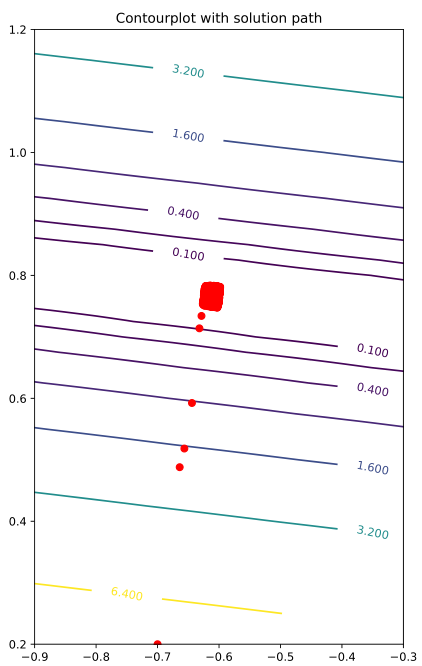
\includegraphics[keepaspectratio, height=\linewidth]{Pictures/stochastic_gradient_descent}
    \captionof{figure}{Stochastic Gradient Descent}
    \label{fig:stochasticgradientdescent}
\end{minipage}

\subsection{Polynomial Regression, Feature Scaling and Checking Convergence}

If we do not have a linear relationship, but a polynomial one between the features and estimated outcome, our equation is in the general form of

\begin{equation}
h(\bm{\theta},\bm{x}) = \theta_0 + \theta_1 x^1 + \theta_2 x^2 + \cdots + \theta_n x^n
\end{equation}

We could then use the features $x_1 = x$, $x_2 = x^2$ and $x_3 = x^3$, but if the features are not in the same range, we have a problem. To solve this we must use feature scaling:

\begin{enumerate}
    \item Make sure the features are on a similar scale and get every feature into the range of $-1\leq x_i \leq 1$
    \begin{enumerate}
        \item Replace $x_i$ with $x_i - \bar{x}_i$ to have features with an approximately zero mean. Does not apply to $x_0 = 1$
        \item Divide $x_i - \bar{x}_i$ by the range of $x_i = max(x_i) - min(x_i)$ or the standard deviation of $x_i$
    \end{enumerate}
    \item Test if Gradient Descent is working correctly by plotting the cost function $J(\bm{\theta})$ versus the number of iterations
    \item Declare convergence if $J(\bm{\theta})$ decreases by less than a given threshold (for example $10^-3$) in one iteration
\end{enumerate}

For sufficiently small $\alpha$, $J(\bm{\theta})$ should decrease in every iteration, but a too small $\alpha$ leads to a slow convergence. Start with $\alpha = 0.001$, proceed with $0.003, 0.01, 0.03, 0.1, ...$ .

\section{Linear Regression}

\begin{wrapfigure}[16]{R}{0.5\textwidth}
    \centering
    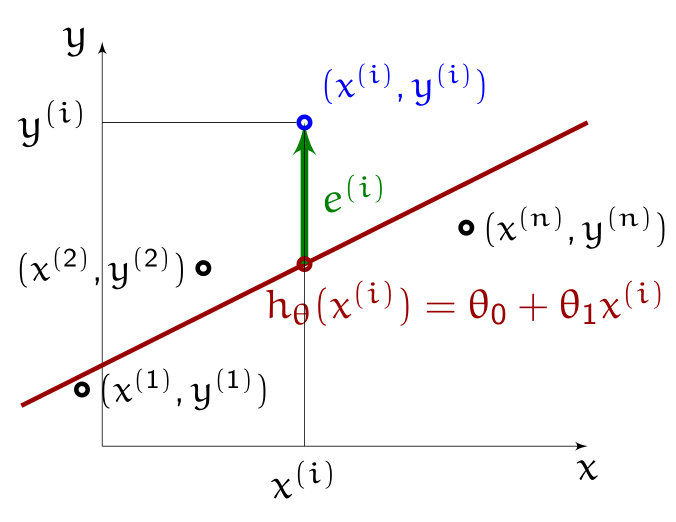
\includegraphics[keepaspectratio=true,height=14\baselineskip]{linear_regression.png}
    \caption{Linear Regression}
    \label{fig:linear_regression}
\end{wrapfigure}

Linear regression is a \textbf{supervised machine learning algorithm} to predict values based on previous variables.

It can also be used to verify whether two variablex X and Y are \textbf{dependant} on each other.

\vspace{10px}

Linear Regression produces a \textbf{straight line} (who would have thought) and each data point has a certain distance from that line. That distance is called \textbf{error} or \textbf{residual}.

These errors should cancel each other out, as the regression-line should be placed in the middle of all the points.

\vspace{10px}

The equation for a 'normal' line is $g(x) = m \cdot x + q$, where $m$ symbolizes the slope of the line and $q$ tells you where the line crosses the $y$-axis.

The equation for the regression line is very much like the 'normal' line-equation, but we use greek symbols, because why not...

\begin{equation}
    h_{\theta}(x) = \theta^{}_{0} + \theta^{}_{1} \cdot x
\end{equation}

\vspace{10px}

As mentioned before, deviation from that line are called errors. Therefore, the error of a given point $i$ can be calculated from the difference of the actual $y_{i}$ from the $h_{\theta}(x)$ (the $y$ on the line)

\begin{equation}
    e_{i} = y_{i} - (\theta^{}_{0} + \theta^{}_{1} \cdot x_{i})
\end{equation}

\vspace{10px}

The goal of linear regression is to find the \textbf{optimal line}, ergo the line that \textbf{produces the smallest errors}.

However, as mentioned earlier, the errors usually cancel each other out, as sometimes the line lies above the data point (negative error) and sometimes it lies below it (positive error). To solve that problem, the parameter we will use to determine the quality of the produced line will be \textbf{the sum of squared error}. By squaring the errors, we can't have negative errors (because squared numbers cannot be negative). Therefore, the smaller the sum of squared errors, the better the line.

The sum of squared errors can be calculated as follows:

\begin{equation}
    J(\theta^{}_{0}, \theta^{}_{1}) = \frac{1}{2n} \sum^{n}_{i=1}(e_{i})^2 = \frac{1}{2n} \sum^{n}_{i=1}[y_{i} - (\theta^{}_{0} + \theta^{}_{1} \cdot x_{i})]^2
\end{equation}

\vspace{10px}

To minimize $J(\theta^{}_{0}, \theta^{}_{1})$, the \textbf{gradient} of $J$ must be \textbf{minimized} or, ideally, zeroed.

This leads to the following formulas for $\theta^{}_{0}$ and $\theta^{}_{1}$

\begin{minipage}{0.45\textwidth}
    \begin{equation}
        \theta^{}_{1} = \frac{S_{xy}}{S_{xx}}
    \end{equation}
\end{minipage} \hfill
\begin{minipage}{0.45\textwidth}
    \begin{equation}
        \theta^{}_{0} = \bar y - \theta^{}_{1} \cdot \bar x
    \end{equation}
\end{minipage}

Where $\bar x$ and $\bar y$ are the \textbf{mean} of the $x$ and $y$ values respectively

\vspace{10px}

$S_{xx}$ and $S_{xy}$ are called \textbf{regression coefficients} and are calculated as follows:

\begin{minipage}{0.45\textwidth}
    \begin{equation}
        S_{xy} = \sum^{n}_{i=1}(x_{i}-\bar x)(y_{i}-\bar y)
    \end{equation}
\end{minipage} \hfill
\begin{minipage}{0.45\textwidth}
    \begin{equation}
        S_{xx} = \sum^{n}_{i=1}(x_{i}-\bar x)^2
    \end{equation}
\end{minipage}

\paragraph{Example} \mbox{}\\

\begin{flalign*}
    &X = [4, 6, 8, 10]& \\
    &Y = [2.3, 4.1, 5.7, 6.9]& \\
    &\bar X = \frac{1}{4} (4 \cdot 6 \cdot 8 \cdot 10) = 7& \\
    &\bar Y = \frac{1}{4} (2.3 \cdot 4.1 \cdot 5.7 \cdot 6.9) = 7.25& \\
    &S_{xx} = (4-7)^2+(6-7)^2+(8-7)^2+(10-7)^2 = 20& \\
    &S_{xy} = (4-7)(2.3-7.25)+(6-7)(4.1-7.25)+(8-7)(5.7-7.25)+(10-7)(6.9-7.25)=15.4& \\
    &\theta^{}_{1} = \frac{20}{15.4} = 0.77& \\
    &\theta^{}_{0} = 4.75-(0.77-7) = -0.64&
\end{flalign*}

From this follows that the regression line is:

\begin{equation*}
    h_{\theta}(x) = -0.64 \cdot 0.77 \cdot x
\end{equation*}

\begin{figure}[htb!]
    \centering
    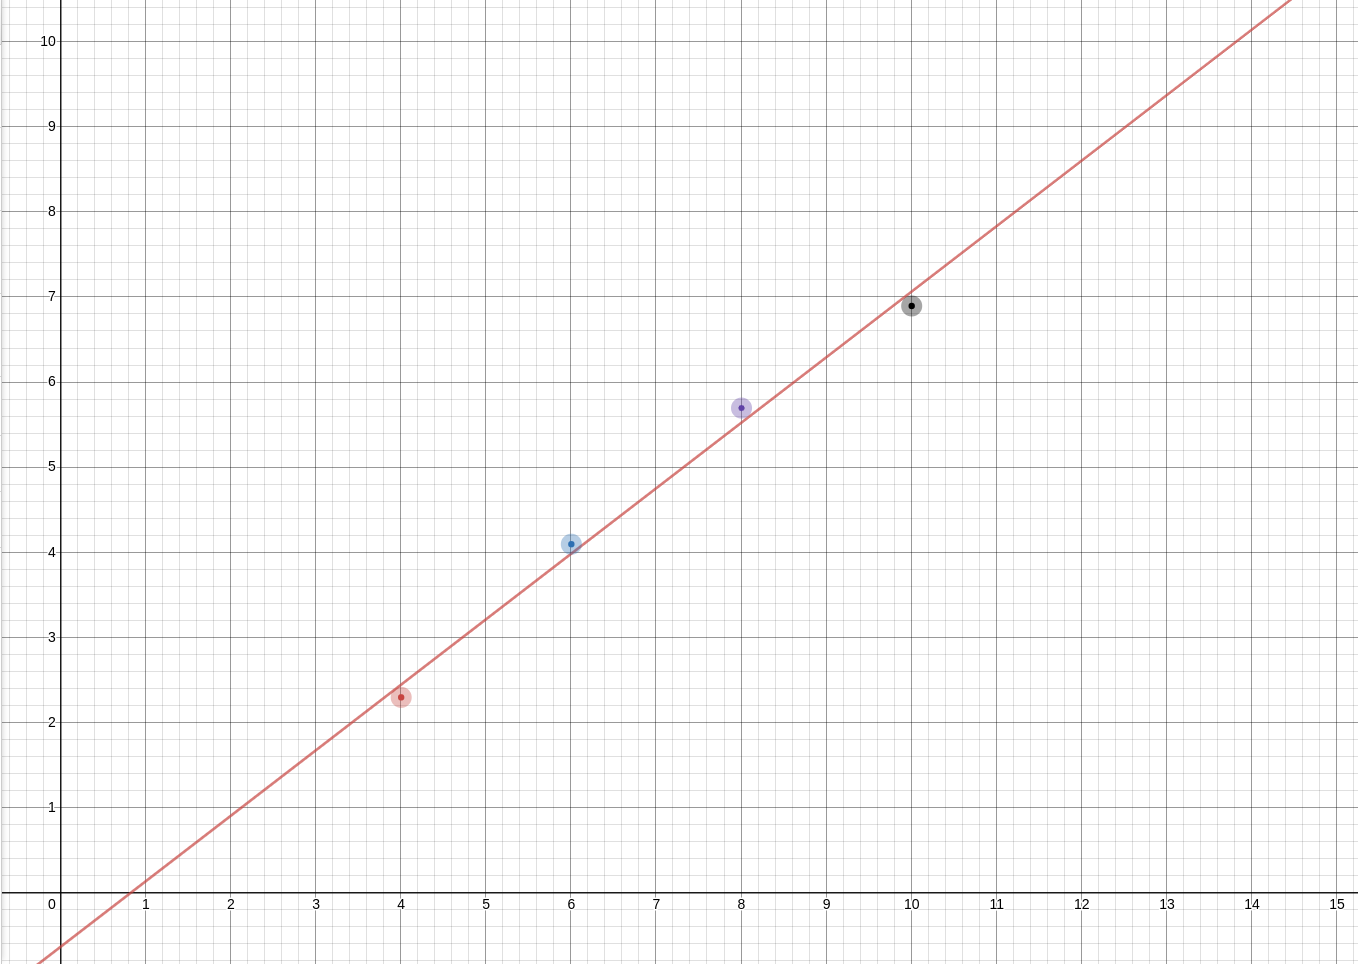
\includegraphics[keepaspectratio=true, width=\linewidth]{regression_line.png}
    \caption{Regression line of the example}
    \label{fig:regression_line}
\end{figure}

From figure \ref{fig:regression_line} we can now see that for $x_{i}=12$, $y$ would most likely be at $8.6$.

\subsection{Coefficient of Determination}

This coefficients was already mentioned in section \ref{sec:r_squared} as 'way to measure how good a regression is'. But how does it even do that?

As mentioned earlier, the goal of a good regression is to \textbf{minimize the sum of squared errors}. However, there are three kinds of sum of squared Errors:

\vspace{10px}

\begin{minipage}{0.4\textwidth}
    \begin{description}
        \item[$\bar y$:] Mean of all $Y$
        \item[$\bar x$:] Mean of all $X$
        \item[$\hat y_{i}$:] Expected value of $y$ based on the regression line
        \item[$y_{i}$:] Actual value of $y$
        \item[$SST:$] \textit{Total sum of squares} \\
              Sum of SSE and SSR
        \item[$SSE:$ ] \textit{Sum of squared Errors} \\
              The sum of the deviations from the predicted points to the regression line
        \item[$SSR:$ ] \textit{Sum of squares explained by regression} \\
              The sum of all deviations from the mean ($\bar y)$ to the regression line
    \end{description}
\end{minipage} \hfill
\begin{minipage}{0.6\textwidth}
    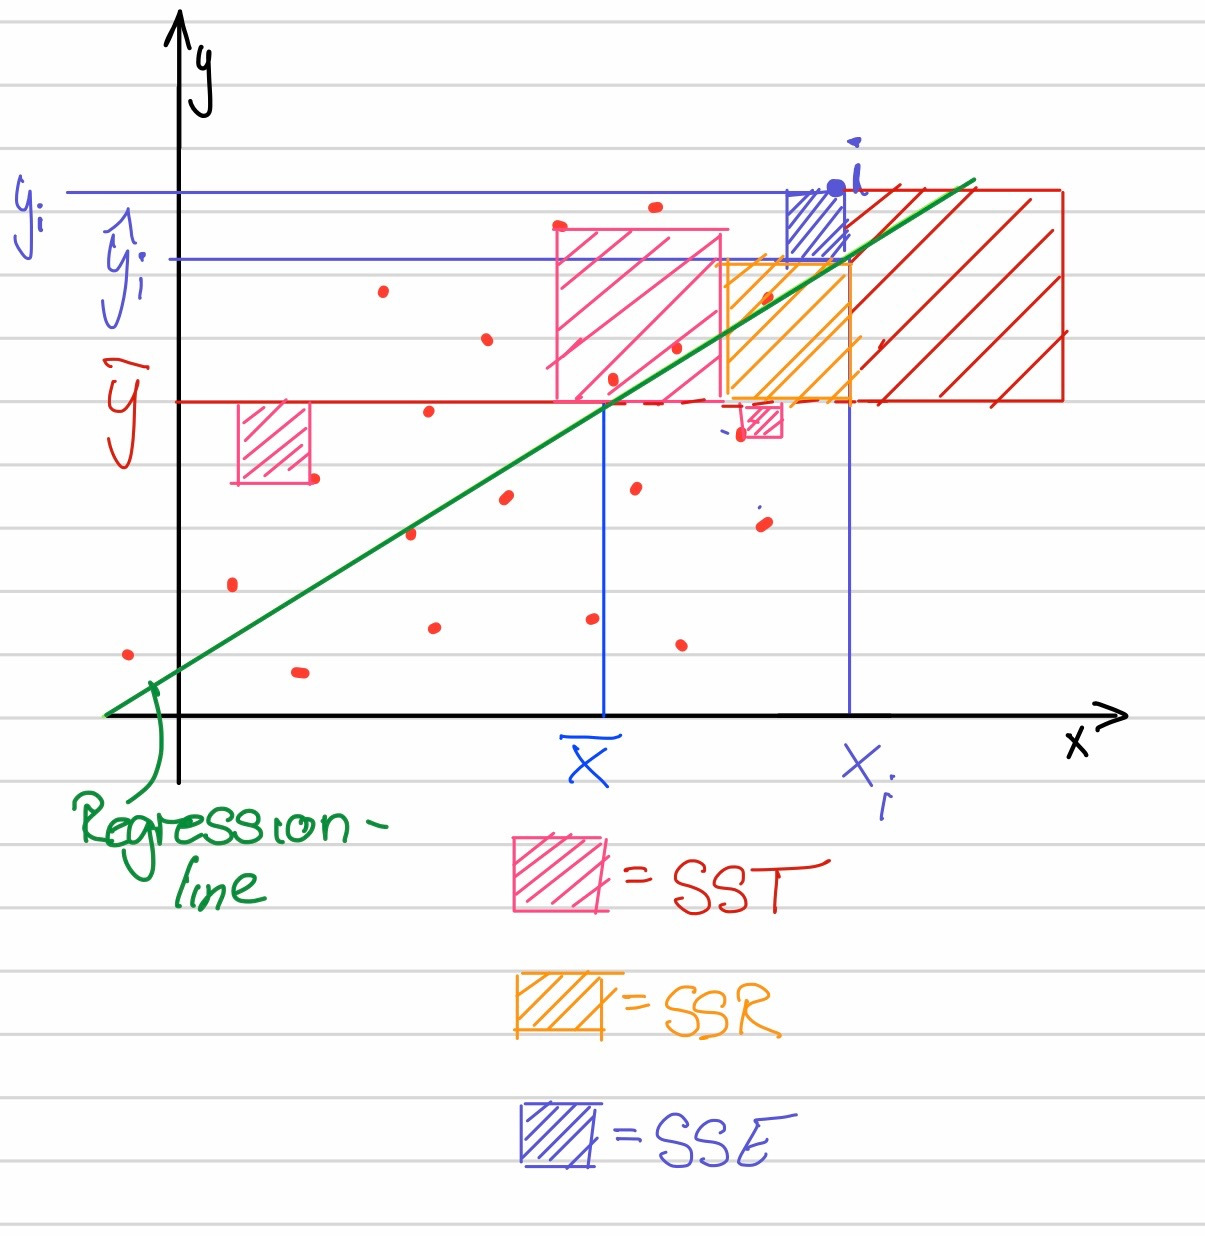
\includegraphics[keepaspectratio=true,width=\textwidth]{SST.JPG}
\end{minipage}

\vspace{10px}

As illustrated in the figure above, $SST = SSR + SSE$.

\begin{align}
    SST &= \sum^{n}_{i=1}(y_{i}-\bar y)^2\\
    SSE &= \sum^{n}_{i=1}(y_{i}-\hat y)^2 &\\
    SSR &= \sum^{n}_{i=1}(\hat y_{i}-\bar y)^2
\end{align}


But how does the aforementioned Coefficient of Determination relate to all of this?

$R^2$ is the \textbf{fraction of the total error that can be explained by the regression}. If all errors can be explained by the regression ($R^2 = 1$), then the regression is perfect

\begin{equation}
    R^2 = \frac{SSR}{SST} = \frac{SST-SSE}{SST} = 1 - \frac{SSE}{SST}
\end{equation}

\vspace{10px}

There's yet another error, the \textit{Mean Squared Error} (MSE). MSE is basically the mean of $SSE$. It is calculated as

\begin{equation}
    MSE = \frac{SSE}{n-2} = \frac{1}{n-2}\sum_{i=1}^{n}(y_{i}-\hat{y}^{}_{i})^2
\end{equation}

\newpage

\subsection{Correlation Analysis}

So now thath you have the regression parameters $\theta^{}_{0}$ and $\theta^{}_{1}$. which make out the regression line. However, that regression line is only as good as your parameters. So how do you test how well you calculated the parameters?

Easy, you calculate the \textbf{standard deviation of these parameters}.

\begin{equation}
    s_{\theta_{0}} = \sqrt{MSE} \cdot \sqrt{\frac{1}{n} + \frac{\bar{x}^2}{\sum_{i=1}^{n}{(x_i-\bar{x})^2}}}
\end{equation}

\begin{equation}
    s_{\theta_{1}} = \sqrt{MSE}\cdot \sqrt{\frac{1}{\sum_{i=1}^{n}{(x_i-\bar{x})^2}}}
\end{equation}

\vspace{10px}

Based on these standard deviations, you can calculate a \textbf{confidence interval}. This interval is a \textbf{degree of uncertainty}. Say we conducted a study and we publish our results with a \textbf{confidence level} of 95\%.

This means that if we used the same sampling method to select different samples and computed an interval estimate for each sample, we would expect the true population parameter to fall within the interval estimates 95\% of the time.

\vspace{10px}

These intervals can be calculated with the aforementioned standard deviation of $\theta^{}_{0}$ and $\theta^{}_{1}$ and some \textit{critical values}. These critical values depend on how high your confidence level and degrees of freedom are.

\begin{figure}[htb!]
    \centering
    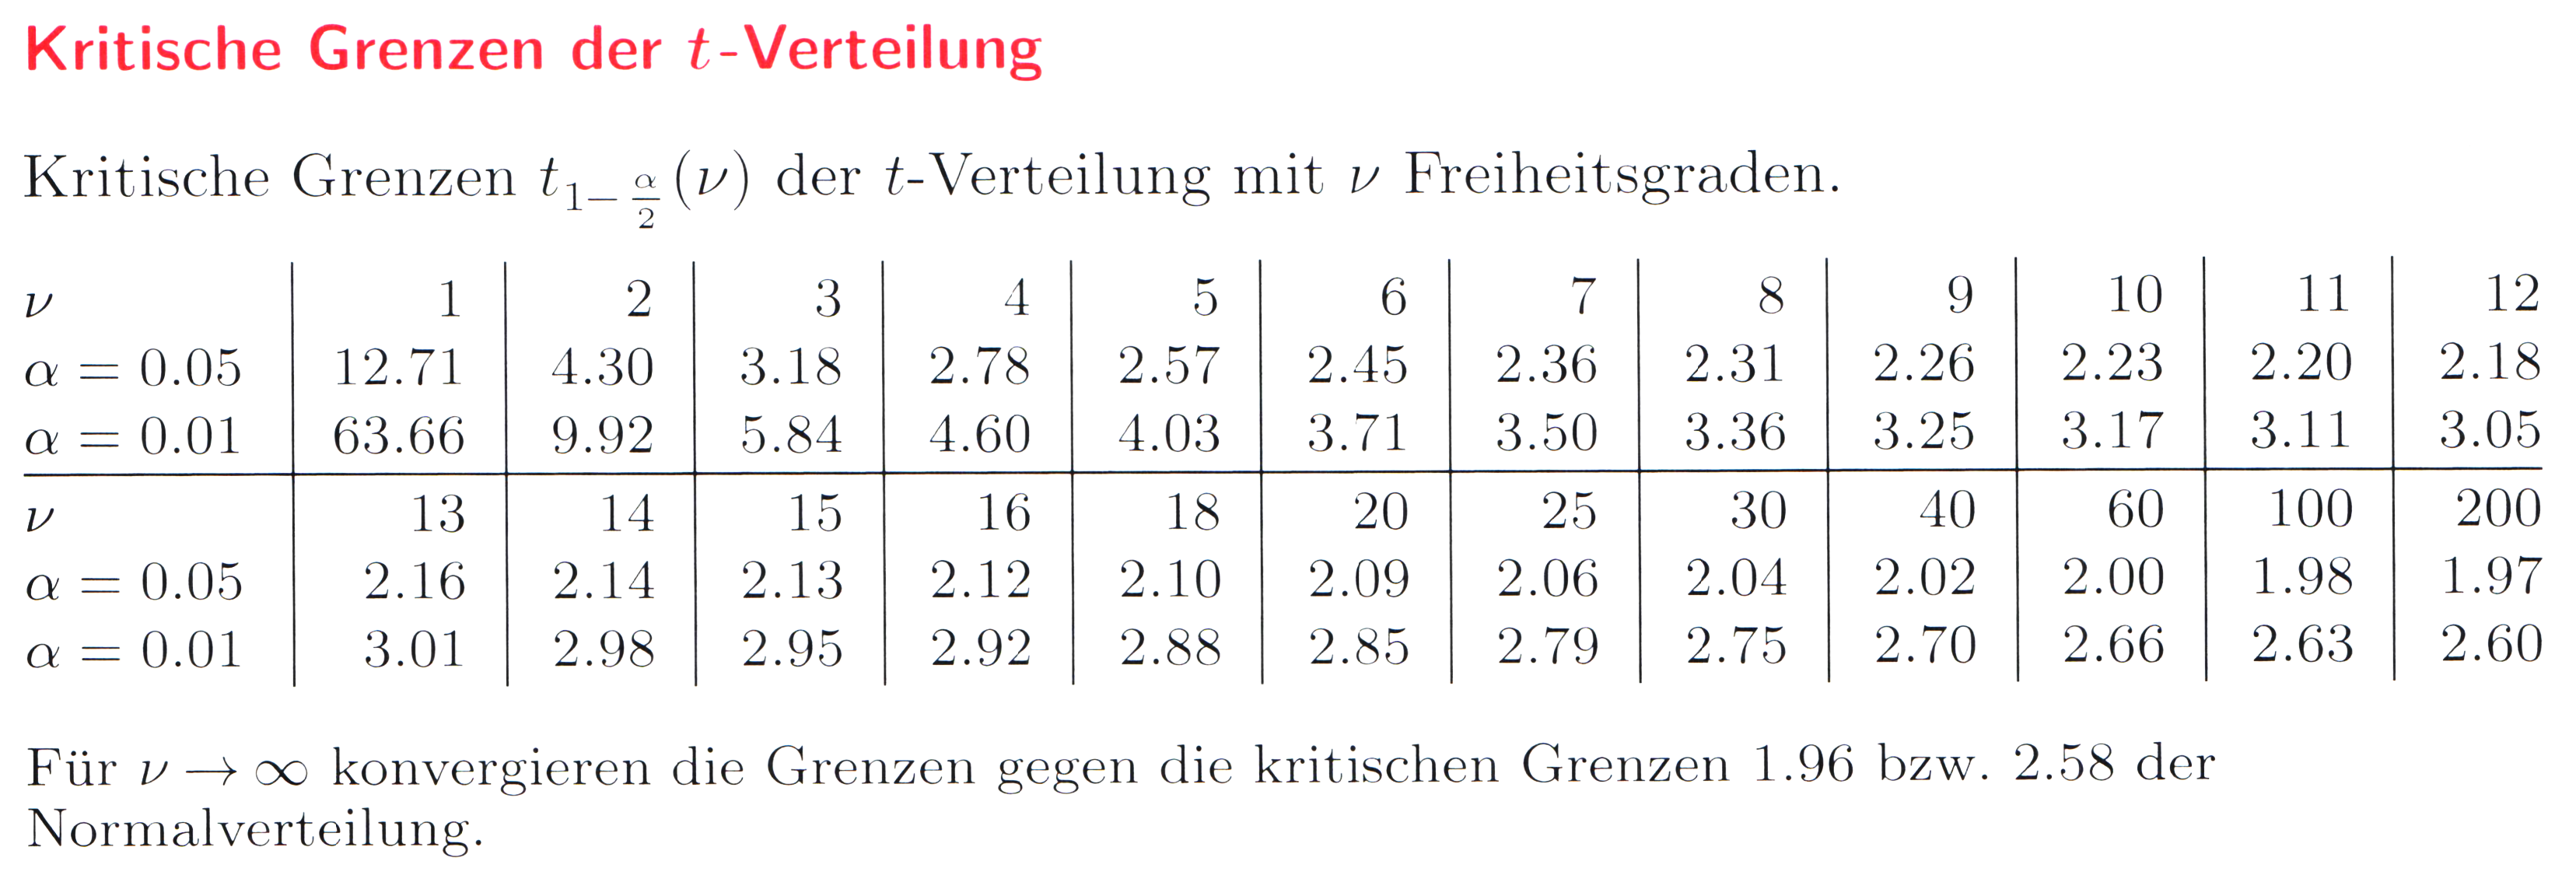
\includegraphics[keepaspectratio=true, width=\linewidth]{CriticalBordersTInterval.png}
    \caption{Critical Values for Confidence Intervals}
    \label{fig:critical_values}
\end{figure}


Degrees of freedom tell you how many regression parameters you already had to calculate. Take for example $SSE$,where both $\theta^{}_{0}$ and $\theta^{}_{1}$ are needed. Therefore, $SSE$ has a degree of freedom of $n-2$, given that you had to calculate 2 parameters.

\vspace{10px}

\noindent Confidence Intervals can be calculated with $[\theta_0 - (critical\ value \cdot \theta_0);\theta_0 + (critical\ value \cdot \theta_0)]$


\newpage

\subsection{Linear Regression Example}

\begin{wrapfigure}[14]{R}{0.4\textwidth}
    \centering
    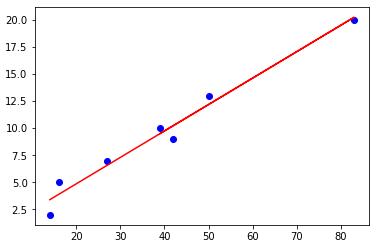
\includegraphics[keepaspectratio=true,height=10\baselineskip]{linear_regression_example.png}
\end{wrapfigure}
\begin{flalign*}
    &X = [14, 16, 27, 42, 83, 50, 39]& \\
    &Y = [2, 5, 7, 9, 20, 13, 10]& \\
\end{flalign*}
\vspace{-40px}
\begin{flalign*}
    &\bar X = \frac{1}{7} \sum^{7}_{i=1}(x_{i}) =
    \frac{14+16+27+42+83+50+39}{7} \\
    &= \frac{271}{7} = \doubleunderline{38.7}& \\
    &\bar Y = \frac{1}{7} \sum^{7}_{i=1}(y_{i}) =
    \frac{2+5+7+9+28+13+10}{7} = \frac{66}{7} = \doubleunderline{9.4}& \\
\end{flalign*}
\vspace{-40px}
\begin{flalign*}
    &S_{xy} = \sum^{7}_{i=1}(x_{i}-\bar x)(y_{i}-\bar y) = (14-38.7)(2-9.4)
    +(16-38.7)(5-9.4)
    +(27-38.7)(7-9.4) \\
    &+(42-38.7)(9-9.4)
    +(83-38.7)(20-9.4)
    +(50-38.7)(13-9.4) \\
    &+(39-38.7)(10-9.4)=\doubleunderline{819} \\
\end{flalign*}
\vspace{-40px}
\begin{flalign*}
    &S_{xx} = \sum^{7}_{i=1}(x_{i}-\bar x)^2 = (14-38.7)^2
    +(16-38.7)^2
    +(27-38.7)^2
    +(42-38.7)^2
    +(83-38.7)^2 \\
    &+(50-38.7)^2
    +(39-38.7)^2 = \doubleunderline{3363.4}
\end{flalign*}
\vspace{-20px}
\begin{flalign*}
    &\theta_1 = \frac{S_{xy}}{S_{xx}} = \frac{819}{3363.4} = \doubleunderline{0.24}&
\end{flalign*}
\vspace{-20px}
\begin{flalign*}
    &\theta_0 = \bar y - \theta_1 \cdot \bar x = 9.4 - 0.24 \cdot 38.7 = \doubleunderline{-0.008}&
\end{flalign*}
\vspace{-20px}
\begin{flalign*}
    &SSE = \sum_{i=1}^{7}(y_{i}-\hat{y}_{i})^2 = \sum_{i=1}^{7}(y_i - (\theta_0 + \theta_1 \cdot x))^2 = \sum_{i=1}^{7}(y_i - (-0.008 + 0.24 \cdot x))^2 \\
    &= \sum_{i=1}^{7}(y_i - (-0.232 \cdot x))^2 = \doubleunderline{5.87}&
\end{flalign*}
\vspace{-20px}
\begin{flalign*}
    &SSR = \sum_{i}^{7}(\hat{y}_{i}-\bar{y})^2 = \sum_{i}^{7}((\theta_0 + \theta_1 \cdot x)-38.7)^2 = \sum_{i}^{7}((-0.008 + 0.24 \cdot x)-38.7)^2 \\
    &= \sum_{i}^{7}((-0.232 \cdot x)-38.7)^2=\doubleunderline{199.84}&
\end{flalign*}
\vspace{-20px}
\begin{flalign*}
    &SST = SSE+SSR = 5.87 + 199.84 = \doubleunderline{205.71}&
\end{flalign*}
\vspace{-20px}
\begin{flalign*}
    &R^2 = \frac{SSR}{SST} = \frac{199.84}{205.71} = \doubleunderline{0.97}&
\end{flalign*}
\vspace{-10px}
\begin{flalign*}
    &MSE = \frac{SSE}{n-2} = \frac{5.87}{7-2}=\doubleunderline{1.17}&
\end{flalign*}
\vspace{-20px}
\begin{flalign*}
    &s_{\theta_{0}} = \sqrt{MSE} \cdot \sqrt{\frac{1}{n} + \frac{\bar{x}^2}{\sum_{i=1}^{n}{(x_i-\bar{x})^2}}} = \sqrt{1.17} \cdot \sqrt{\frac{1}{7} + \frac{38.7^2}{\sum_{i=1}^{n}{(x_i-38.7)^2}}} = \doubleunderline{-0.008}&
\end{flalign*}
\vspace{-10px}
\begin{flalign*}
    &s_{\theta_{1}} = \sqrt{MSE}\cdot \sqrt{\frac{1}{\sum_{i=1}^{n}{(x_i-\bar{x})^2}}} = \sqrt{1.17} \cdot \sqrt{\frac{1}{\sum_{i=1}^{n}{(x_i-38.7)^2}}} = \doubleunderline{0.019}& &
\end{flalign*}
\vspace{-10px}
\begin{flalign*}
    &Interval\ \theta_0 = [\theta_0 - 2.57 \cdot \theta_0; \theta_0 + 2.57 \cdot \theta_0] = \doubleunderline{[-2.14;2.12]} &
\end{flalign*}
\vspace{-20px}
\begin{flalign*}
    &Interval\ \theta_1 [\theta_1 - 2.57 \cdot \theta_1; \theta_1 + 2.57 \cdot \theta_1] = \doubleunderline{[0.20;0.29]}&
\end{flalign*}

\newpage
\restoregeometry


The results of the last page can also be achieved with the following python-code:

\begin{lstlisting}
import matplotlib.pyplot as plt
import scipy.stats as st
import seaborn as sns
import pandas as pd
import numpy as np

%precision 10
%matplotlib inline

x=np.array([14, 16, 27, 42, 83, 50, 39])
y=np.array([2, 5, 7, 9, 20, 13, 10])

mean_x = np.mean(x)
mean_y = np.mean(y)

Sxx = np.sum((x-mean_x)**2)
Syy = np.sum((y-mean_y)**2)
Sxy = np.sum((x-mean_x)*(y-mean_y))

thet1 = Sxy/Sxx
thet0 = mean_y-thet1*mean_x

# To show the regression line
plt.plot(x,y, 'bo')
plt.plot(x,thet0+thet1*x, 'r')
plt.show()

hat_y = thet0+thet1*x

SSE=np.sum(((y-hat_y))**2)

SSR=np.sum((hat_y-mean_y)**2)

SST = SSE + SSR

R_sq = SSR/SST

MSE = SSE/(len(x)-2)

Sthet0 = np.sqrt(MSE)*np.sqrt((1/len(x))+(mean_x**2)/(np.sum((x-mean_x)**2)))

Sthet1 = (np.sqrt(MSE))*np.sqrt(1/(np.sum((x-mean_x)**2)))

print("theta_1: " + str(thet1))

print("Interval theta0: [" + str(thet0 - (2.57*Sthet0)) + " ; " + str(thet0 + (2.57*Sthet0)) + "]")

print("Interval theta1: [" + str(thet1 - (2.57*Sthet1)) + " ; " + str(thet1 + (2.57*Sthet1)) + "]")

\end{lstlisting}



\subsection{Multple Linear Regression}

Linear Regeression is great and all, but what if you wanted to predict an independent value based on \textbf{multiple} other values? In that case we would need \textbf{multilinear regression}.
\noindent
In Muliple Linear Regression we try to fit a plane instead of a line. This plane is defined by
\begin{equation}
    y = h_\theta(x_1,x_2) = \theta_0 + \theta_1 x_1 + \theta_2 x_2
\end{equation}
And mapped to the sample with index $i$
\begin{equation*}
    y_i = \theta_0 + \theta_1 x_{1,i} + \theta_2 x_{2,i} + e_i
\end{equation*}

This can be transformed to matrices

\begin{equation*}
    \begin{bmatrix}
        y_1    \\
        y_2    \\
        \vdots \\
        y_n
    \end{bmatrix}
    =
    \begin{bmatrix}
        1 & x_{1,1} & x_{2,1} \\
        1 & x_{1,2} & x_{2,2} \\
          & \vdots  &         \\
        1 & x_{1,n} & x_{2,n} \\
    \end{bmatrix}
    \begin{bmatrix}
        \theta_0 \\
        \theta_1 \\
        \theta_2
    \end{bmatrix}
    +
    \begin{bmatrix}
        e_1    \\
        e_2    \\
        \vdots \\
        e_n
    \end{bmatrix}
\end{equation*}

This can be solved as follows

\begin{equation*}
    \bm{\theta} = (\bm{X}^T\bm{X})^-1\bm{X}^T\bm{y}
\end{equation*}

In more than three dimensions our plane becomes a hyperplane, and the model is

\begin{equation*}
    y_i = \theta_0 + \theta_1 x_{1,i} + \theta_2 x_{2,i} + \cdots + \theta_m x_{m,i}  + e_i=\sum_{k=0}^{n}\theta_k x_{k,i} + e_i
\end{equation*}

\subsubsection{Example multilinear regression}

Suppose we want to predict the weight of a weightlifter based on the training hours per week and the delivery of protein.

\vspace{10px}

\begin{minipage}{0.25\textwidth}
    \begin{tabular}{cccc}
        \toprule
        \thead{i} & \thead{y} & \thead{$x_1$} & \thead{$x_2$} \\
        \hline
        1         & 93        & 2             & 1.1           \\
        \hline
        2         & 106       & 2             & 1.9           \\
        \hline
        3         & 146       & 4             & 2             \\
        \hline
        4         & 140       & 5             & 1.5           \\
        \hline
        5         & 151       & 6             & 1.3           \\
        \hline
        6         & 158       & 7             & 2.1           \\
        \hline
        7         & 130       & 4             & 1.8           \\
        \hline
        8         & 159       & 5             & 2.5           \\
        \bottomrule
    \end{tabular}
\end{minipage}\hfill
\begin{minipage}{0.75\textwidth}
    \begin{description}
        \item[$i$: ] No. of observation
        \item[$y$: ] Weight in kg
        \item[$x_1$: ] Training h/week
        \item[$x_2$: ] Protein intake g/kg/day
    \end{description}

    We assume that the function to calculate the weight from training-hours and protein intake is as follows:
\end{minipage}

\vspace{10px}

\begin{equation*}
    y = h_\theta (x_1, x_2) = \theta_0 + \theta_1 \cdot x_1 + \theta_2 \cdot x_2
\end{equation*}

\begin{figure}[htb!]
    \centering
    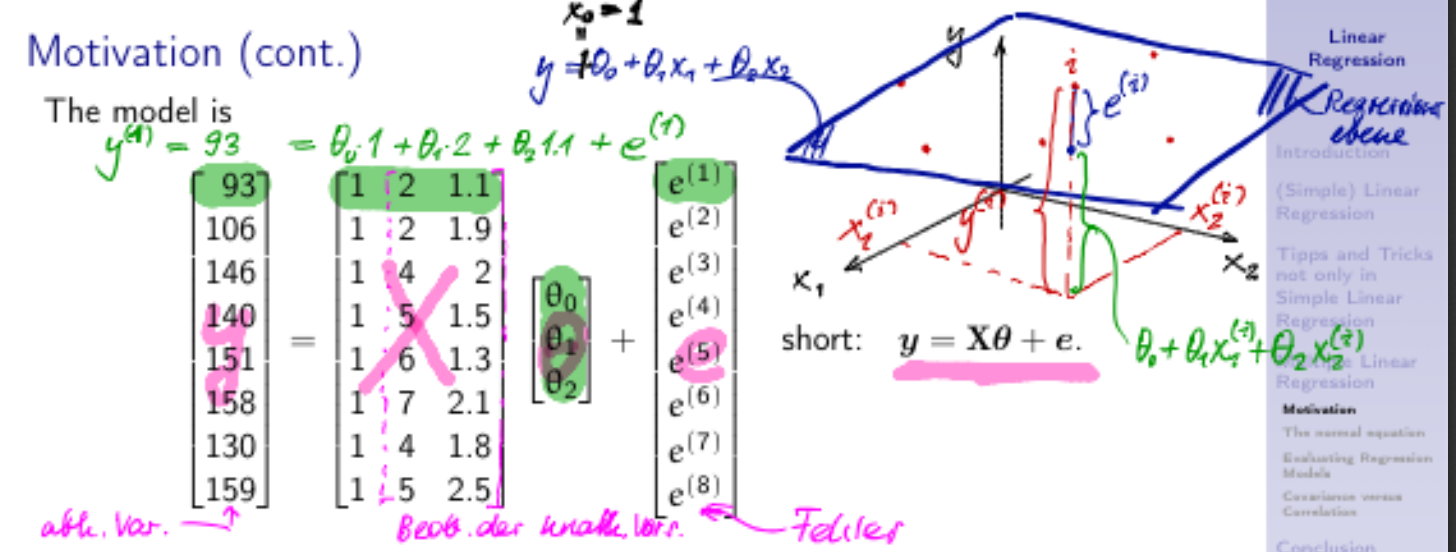
\includegraphics[keepaspectratio=true, width=\linewidth]{multilinear_regression.png}
    \caption{Model of the multilinear regression (\textcopyright J. Bürgler, 2019)}
    \label{multilinear_regression}
\end{figure}

The following solution  minimizes the sum of squared errors in this model (and therefore get a hella good regression).

\begin{equation*}
    \theta = (X^T X)^{-1} X^T y =
    \begin{bmatrix}
        \theta_0 \\
        \theta_1 \\
        \theta_2
    \end{bmatrix}
    \rightarrow
    \begin{bmatrix}
        55.7 \\
        11.1 \\
        17.5
    \end{bmatrix}
\end{equation*}

According to this, the regression plane would be:
\begin{equation*}
    y = h_\theta (x_1, x_2) = 55.7 + 11.1 \cdot x_1 + 17.5 \cdot x_2
\end{equation*}

\newpage

Of course, this can also be done rather easily in Python:

\begin{lstlisting}
import numpy as np

X = np.matrix([[2,1.1],[2,1.9],[4,2.0],[5,1.5],[6,1.3],[7,2.1],[4,1.8],[5,2.5]])

# Anzahl Reihen von X anhand der ersten Zeile (= Anzahl Beobachtungen)
n = X.shape[0]

y = np.matrix([93,106,146,140,151,158,130,159])

# Append a column of '1' infront of the X-matrix (to get the 'X'-matrix from the figure) 
X_ext = np.c_[np.ones((n,1)),X]

theta = np.linalg.inv(X_ext.T.dot(X_est)).dot(X_ext.T).dot(y)

print(theta)
\end{lstlisting}


\section{Regularisation}
Under- and overfitting are common problems in machine learning. Underfitting occurs when the model is to general and can't aptly represent the data. Overfitting occurs, when the model is too precisely fitted to the training data.

\begin{figure}[htb!]
    \centering
    \begin{subfigure}{0.6\linewidth}
        \centering
        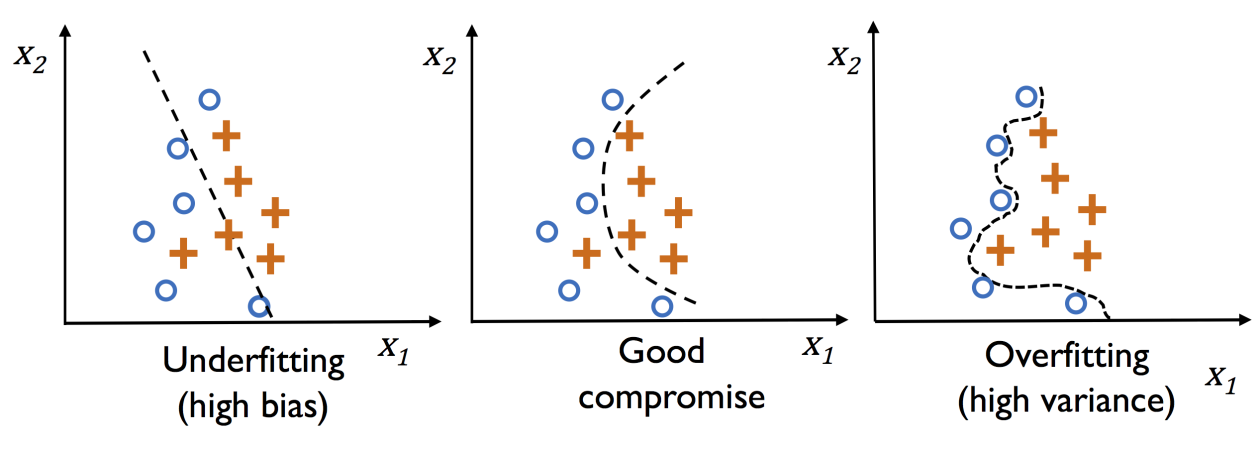
\includegraphics[keepaspectratio,width=\linewidth]{Pictures/under_and_overfitting}
        \caption{Example of different fittings}
    \end{subfigure}
    \begin{subfigure}{0.6\linewidth}
        \centering
        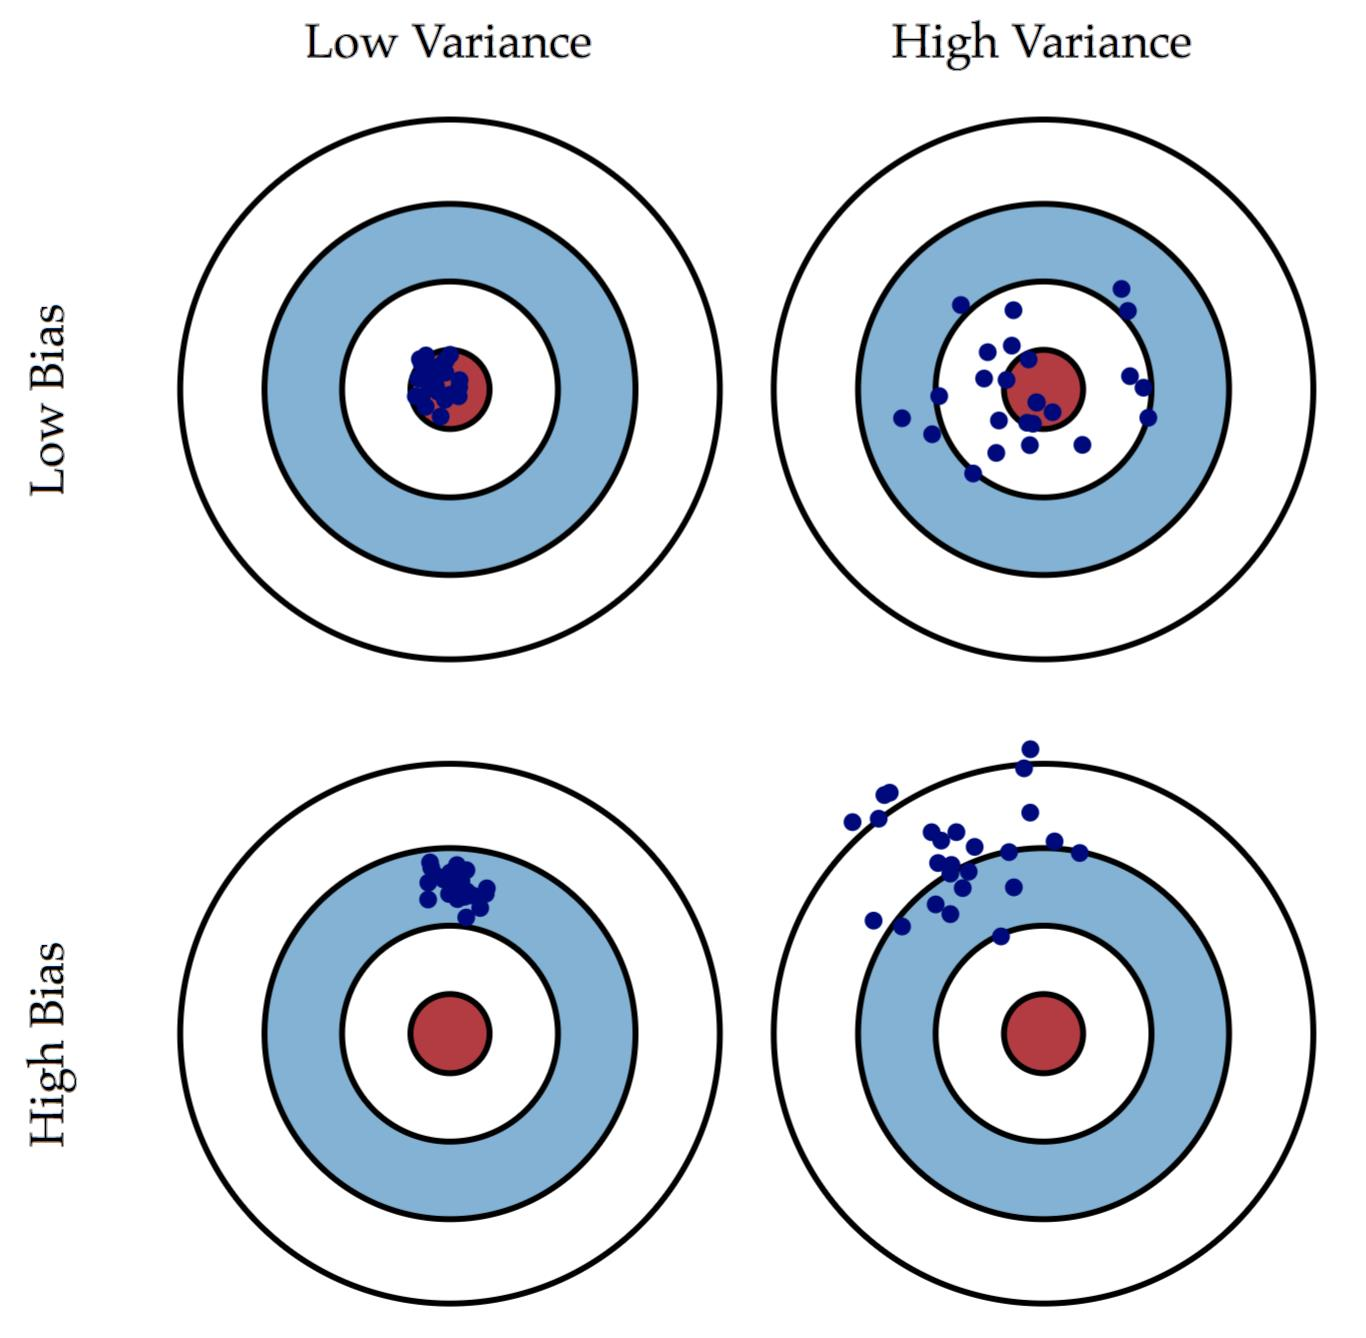
\includegraphics[keepaspectratio,width=\linewidth]{Pictures/biases_and_variances}
        \caption{Examples of different biases and variances}
    \end{subfigure}
    \caption{Under- and Overfitting, Biases and Variances}
\end{figure}

To address overfitting we can try these approaches
\begin{enumerate}
    \item Reduce the number of features
          \begin{itemize}
              \item Manually select which features to keep
              \item Model selection algorithm
          \end{itemize}
    \item Regularisation
          \begin{itemize}
              \item Keep all features, but reduce magnitude of parameters $\theta_i$
              \item Works well with lots of features which each contribute just a bit to predict y
          \end{itemize}
\end{enumerate}

\subsection{Ridge Regularisation}
\begin{equation}
    J(\theta) = \frac{1}{2n}\left[\sum_{i=1}^{n}(h(\theta,x_i)-y_i)^2 + \lambda \sum_{j=1}^{m}\theta_j^2\right]
\end{equation}

The second sum goes from $1$ to the number of features $m$ and it does not contain $\theta_0$. The regularisation hyperparameter $\lambda$ controls the amount of regularisation. If $\lambda = 0$ there will be no regularization, and if $\lambda = \infty$ there will be underfitting because only $\theta_0$ will be different from zero.
In Ridge regularised regression, we choose $\theta$ to minimize $J(\theta)$:
\begin{equation}
    \hat{\theta} = \underset{\theta}{\text{argmin}} J(\theta)
\end{equation}

\begin{itemize}[leftmargin=*, labelindent=3cm, labelsep=1cm]
    \item[large $\lambda$] High Bias / Underfit
    \item[intermediate $\lambda$] Correct
    \item[small $\lambda$] High Variance / Overfit
\end{itemize}

\subsection{How to choose the right model}

\subsubsection{Hold-out / Simple Cross Validation}
\begin{enumerate}
    \item Randomly split the Sample $S$ into $S_{train}$ and $S_{cv}$ called the \textbf{hold-out cross validation set}. A standard split is 70\% $S_{train}$ and 30\% $S_{cv}$.
    \item For each degree of the polynomial $k$, train the model $M_k$ on $S_{train}$ to get the parameter vector $\bm{\theta}_k$
    \item Select $\bm{\theta}_k$ with the smallest error $\hat{\varepsilon}_{S_{cv}}(\bm{\theta}_k)$
          \begin{equation*}
              k = \underset{k\in{1,2,...,10}}{\text{argmin}}\hat{\varepsilon}_{S_{cv}}(\bm{\theta}_k)
          \end{equation*}
          where $\hat{\varepsilon}_{S_{cv}}(\bm{\theta}_k)$ is the empirical error, if we use $\bm{\theta}_k$ as the parameter vector on the cross validation set $S_{cv}$.
\end{enumerate}

The issue with \textbf{hold-out cross validation} is, that it wastes the amount of data used for the cross validation.

\subsubsection{k-fold Cross Validation}

To reduce the waste of data, we could hold out less data used per run: we use k-fold cross validation \textbf{k-fold cross validation}.

\begin{enumerate}
    \item Randomly split $S$ into $l$ disjoint subsets $S_1, S_2, ... , S_l$ of $\frac{n}{l}$ training examples each
    \item Evaluate each model $M_k, k\in{1,2, ... , 10}$ as follows
          \begin{itemize}
              \item For $j=1,2,...,l$ train $M_k$ on all data, except the subset $S_j$ to get $\bm{\theta}_{kj}$ and test $\bm{\theta}_{kj}$ on $S_j$ to get the empirical error $\hat{\varepsilon}_{S_j}(\bm{\theta}_{kj})$
              \item The estimated generalisation of the model $M_k$ is then calculated as the average of the $\hat{\varepsilon}_{S_j}(\bm{\theta}_{kj})$
                    \begin{equation*}
                        \frac{1}{l}\sum_{j=1}^{l}\hat{\varepsilon}_{S_j}(\bm{\theta}_{kj}) \text{ where } \hat{\varepsilon}_{S_j}(\bm{\theta}_{kj})=\frac{1}{2n}\sum_{i=1}^{n}(h(\bm{\theta}_k,\bm{x}^{(i)})-y^{(i)})^2
                    \end{equation*}
          \end{itemize}
    \item Pick the model $M-K$ with the lowest estimated generalisation error and retrain that model on the entirety of the training set $S$.
\end{enumerate}

\section{Support Vector Machines}

\subsection{Scalar Product}
The scalar product between two vectors $\vec{a}, \vec{b}$ is defined as
\begin{equation}
\vec{a}\cdot\vec{b}=\sum_{i=1}^{n}a_i b_i = a_1 b_1 + a_2 b_2 + \cdots + a_n b_n
\end{equation}
\noindent
The following rules hold true for the scalar product

\begin{itemize}[leftmargin=*, labelindent=5cm, labelsep=0.5cm]
	\item[\textbf{symmetry}] $\vec{a}\cdot\vec{b} = \vec{b}\cdot\vec{a}$
	\item[\textbf{distributivity}] $\vec{a}\cdot(\vec{b}+\vec{c}) = \vec{a}\cdot\vec{b} + \vec{a}\cdot\vec{c} $
	\item[\textbf{multiplication by scalars}] $\lambda(\vec{a}\cdot\vec{b}) = (\lambda\vec{a})\cdot\vec{b} = \vec{a}\cdot(\lambda\vec{b})$
\end{itemize}
\noindent
Using the scalar product we can define the length of a vector, also called the $\text{L}^2$-Norm

\begin{equation}
\| \vec{a} \| = \sqrt{a_1^2 + a_2^2 + \cdots + a_n^2} = \sqrt{\vec{a}\cdot\vec{a}}
\end{equation}
\noindent
Two vectors are orthogonal if and only if their scalar product is zero:
\begin{equation}
\vec{a}\cdot\vec{b} = 0 \Leftrightarrow \vec{a} \perp \vec{b}
\end{equation}

\paragraph{Example of scalar product}
\begin{equation*}
\begin{bmatrix}1\\2\end{bmatrix}\cdot\begin{bmatrix}3\\4\end{bmatrix} = 1\cdot 3 + 2\cdot 4 = 11
\end{equation*}

\subsubsection{The Hessian normal form of a straight line}

The straight line $g$ is defined by some point $x_0$ and the normal vector $\vec{n}$ with length 1 (refer to figure \ref{fig:hessiannormalform}).

\begin{figure}[htb!]
	\centering
	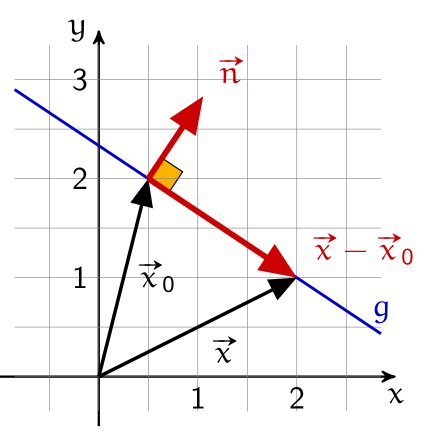
\includegraphics[keepaspectratio, width=0.4\linewidth]{Pictures/Hessian_normal_form}
	\caption{Plot of $g$ and the relevant vectors $\vec{x_0}$ and $\vec{n}$}
	\label{fig:hessiannormalform}
\end{figure}
\noindent
For any point $x$ on the line we have
\begin{equation*}
\vec{n}\cdot(\vec{x}-\vec{x_0})=0
\end{equation*}
\noindent
And find
\begin{equation*}
\Rightarrow n_x x + n_y y -(n_x x_0  n_y y_0) = n_x x +n_y y + d = 0
\end{equation*}
\noindent
With $d=-(n_x x_0 +n_y y_0)$ the signed distance $-\vec{n}\cdot\vec{x_0}$ from the origin

The generalisation of the Hessian normal form to a plane in 3D-space is straight forward:
\begin{equation}
\vec{n}\cdot(\vec{x} - \vec{x_0}) = 0 \text{ \textbf{or} } \vec{n}\cdot\vec{x} + d = 0\text{ with } d = -\vec{n}\cdot\vec{x_0}
\end{equation}

\paragraph{Example of the Hessian Normal Form}
The line $g$ is taken from figure \ref{fig:hessiannormalformexample}

\begin{figure}[tbh!]
	\centering
	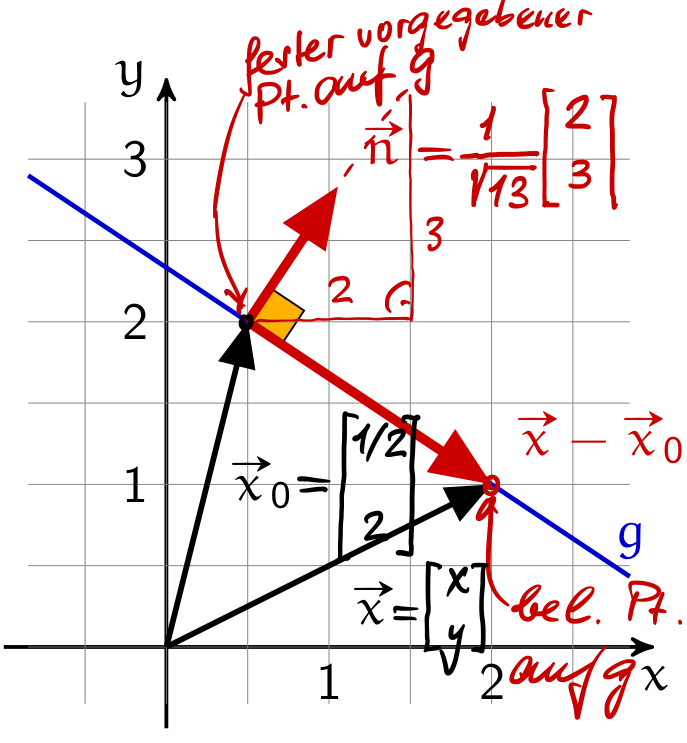
\includegraphics[width=0.5\linewidth, keepaspectratio]{Pictures/hessian_normal_form_example}
	\caption{Annotated figure \ref{fig:hessiannormalform}}
	\label{fig:hessiannormalformexample}
\end{figure}

\begin{align*}
\vec{n} &= \frac{1}{\sqrt{13}} \begin{bmatrix}2\\3\end{bmatrix}\\
0 &= \vec{n}\cdot(\vec{x}-\vec{x_0})\\
&= \frac{1}{\sqrt{13}} \begin{bmatrix}2\\3\end{bmatrix} \cdot(\begin{bmatrix}x\\y\end{bmatrix} - \begin{bmatrix}0.5\\2\end{bmatrix})\\
&= \frac{1}{\sqrt{13}} \begin{bmatrix}2\\3\end{bmatrix} \cdot \begin{bmatrix}x - 0.5\\ y - 2\end{bmatrix}
\end{align*}

\subsubsection{Motivation for Support Vector Machines}

\begin{itemize}
	\item Classifying data means splitting it up
	\item There are many ways to split the data, even using only a linear function
	\item We want the best possible split
\end{itemize}

\begin{figure}
	\centering
	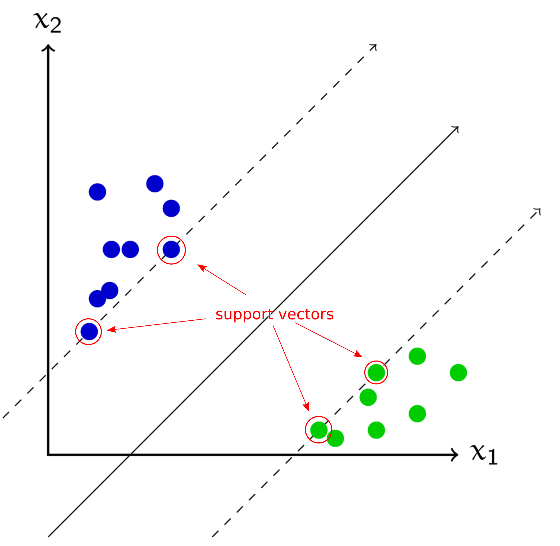
\includegraphics[keepaspectratio,width=0.4\linewidth]{Pictures/support_vector_machine_ex1}
	\caption{Support Vector Machine}
	\label{fig:supportvectormachineex1}
\end{figure}

The line in the middle of figure \ref{fig:supportvectormachineex1} is called the hyperplane (a line in two dimensions, a plane in three). We know that this is the best possible split, because it is the furthest from both clusters. The data points (samples) closest to the hyperplane are called support vectors.

\subsection{Basic ideas and features}

\begin{itemize}
	\item Finds optimal hyperplane for linearly separable patterns
	\item Extended patterns which are not linearly separable are transformed into another (possibly higher dimensional) feature space
	\item Not affected by the local minima problem
	\item No dimensionality problem
	\item Modular design allows separate implementation of various components
	\item Support vectors are the data points or samples closest to the decision hyperplane
	\item Support vectors are the most difficult to classify
	\item Support vectors directly influence the position of the decision hyperplane and are the critical elements in the training set
	\item Problem of finding an optimal separating hyperplane can be solved using standard optimisation techniques
\end{itemize}

\subsubsection{Linear Classifier}
A linear classifier has the form
\begin{equation}
f(\vec{x}) = \theta_0 + \theta_1 x_1 + \cdots + \theta_m x_m = b + w_1 x_1 + w_2 x_2 + \cdots + w_m x_m = b + \vec{w}^T \vec{x}_b
\end{equation}
\noindent
where $\vec{w} = \begin{bmatrix}
\theta_0\\\theta_1\\\vdots\\\theta_m
\end{bmatrix}$ is the normal vector on the hyperplane and $b = \theta_0$ is the bias.

\subsubsection{How to determine optimality}

\begin{figure}[htb!]
	\centering
	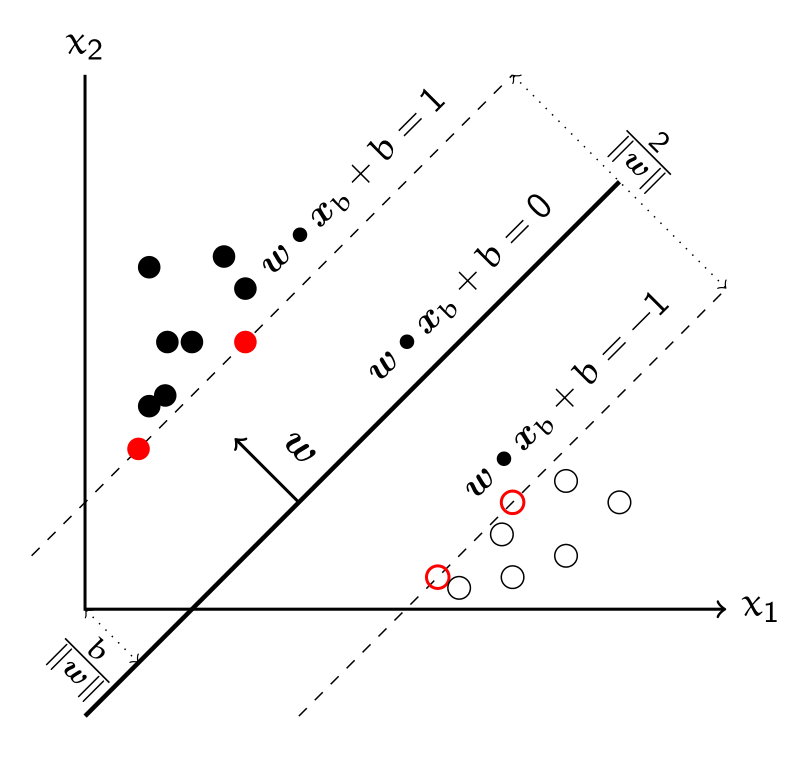
\includegraphics[keepaspectratio, width=0.4\linewidth]{Pictures/support_vector_machine_hyperplane}
	\caption{Hyperplane with support vectors in red}
	\label{fig:supportvectormachinehyperplane}
\end{figure}

In figure \ref{fig:supportvectormachinehyperplane} $\vec{w}$ is the normal vector on the decision hyperplane, its length depends on the margin which is
maximised through the Support Vector Machine. Maximising the margin $\frac{2}{\| \vec{w} \|}$ is equivalent to minimising $\frac{\vec{w}^T \vec{w}}{2}$, therefore we
\begin{equation}\label{eq:hard_margin_problem}
\underset{\vec{w}, b}{\text{minimise}}\ \frac{1}{2}\vec{w}^T \vec{w}
\end{equation}
\noindent
subject to $y^{(i)}(\vec{w}^T \vec{x}^{(i)}+b)\geq 1$ for $i = 1,2,...,n$

% TODO Dual SVM derivation?

\subsection{From the hard margin to the soft margin problem}

So far we have discussed the hard margin problem (see equation \ref{eq:hard_margin_problem}), which fails if the problem is not separable. To address this we could introduce a \textbf{slack variable} $\zeta_i$ for each data point $x^{(i)}$ and solve the \textbf{soft margin problem}

\begin{equation}\label{eq:soft_margin_problem}
\underset{\vec{w}, b}{\text{minimise}}\ \frac{1}{2}\vec{w}^T \vec{w} + C\sum_{i=1}^{n}\zeta_i \text{ subject to } y^{(i)}(\vec{w}^T \vec{x}^{(i)} + b) \geq 1 - \zeta_i
\end{equation}
\noindent
with $\zeta_i \geq 0$ for $i=1,2,...,n$. The slack variable $\zeta_i$ measures how much the $i$-th instance $\vec{x}^{(i)}$ is allowed to violate the margin.

\begin{figure}
	\centering
	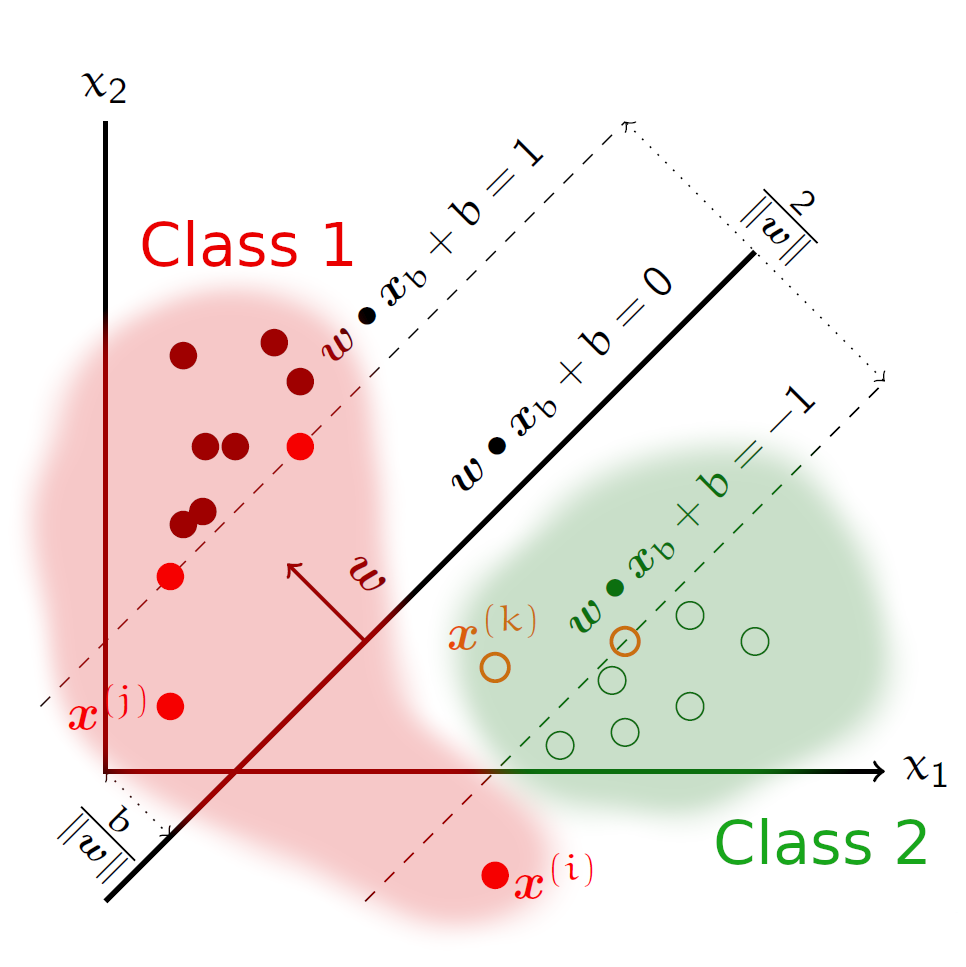
\includegraphics[keepaspectratio,width=0.4\linewidth]{Pictures/soft_margin_svm}
	\caption{Support Vector Machine with soft margins}
	\label{fig:svm_softmargins}
\end{figure}

\subsubsection{The slack variable explained}

The margin can be less than 1, by setting $\zeta_i > 0$, but then this gets factored in as a penalty $C\zeta_i$ in the minimisation. Thus the sum $\sum_{i=1}^{n}\zeta_i$ gives an upper bound on the number of training errors. With this soft margin Support Vector Machines minimise training error traded off against better margins. The parameter $C$ is the \textit{regularisation parameter}, which provides a way to control overfitting:

\begin{itemize}[leftmargin=*, labelindent=5cm, labelsep=0.5cm]
	\item[small $C$ ($C \rightarrow 0$)] Constraints are easily ignored, we obtain a large margin
	\item[large $C$ ($C \rightarrow \infty$)] Constraints are hard to ignore, we obtain a narrow margin
	\item[$C = \infty$)] All constraints enforced, we have a hard margin
\end{itemize}

Therefore we still have a quadratic optimisation problem with a unique minimum and we only have to deal with the parameter $C$.

\subsection{The Kernel Trick}

The kernel transforms a problem to another coordinate system, where the problem may be linearly separable.

\begin{figure}[htb!]
	\centering
	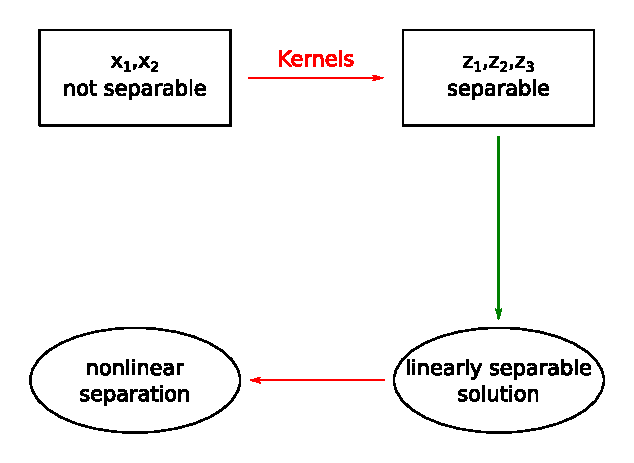
\includegraphics[keepaspectratio, width=0.5\linewidth]{Pictures/KernelTrick.pdf}
	\caption{Course of action for the kernel method}
	\label{fig:kerneltrick}
\end{figure}

\subsubsection{Kernel Functions Examples}

\begin{itemize}[leftmargin=*, labelindent=3.5cm, labelsep=0.5cm]
	\item[polar coordinates] $\Phi: \mathbb{R}^2 \rightarrow \mathbb{R}^2, \begin{bmatrix}x_1\\x_2\end{bmatrix}\mapsto\begin{bmatrix}r\\\theta\end{bmatrix}=\begin{bmatrix}\sqrt{x_1^2 + x_2^2}\\\arctan(\frac{x_2}{x_2})\pm\pi\end{bmatrix}$ (refer to figure \ref{fig:kernelfunctionspolarcoordinates})
	\item[polynomial mapping] $\Phi: \mathbb{R}^2 \rightarrow \mathbb{R}^3, (x_1,x_2) \mapsto (z_1,z_2,z_3) = (x_1^2,\sqrt{2}\cdot x_1\cdot x_2, x_2^2) = \Phi(x_1,x_2)$ (refer to figure \ref{fig:kernelfunctionspolynomialmapping})
	\item[radial] $\Phi(x_1,x_2) = e^{-\frac{\| x_1 - x_2 \|^2}{2\sigma^2}}$
\end{itemize}

\begin{figure}[htb!]
	\centering
	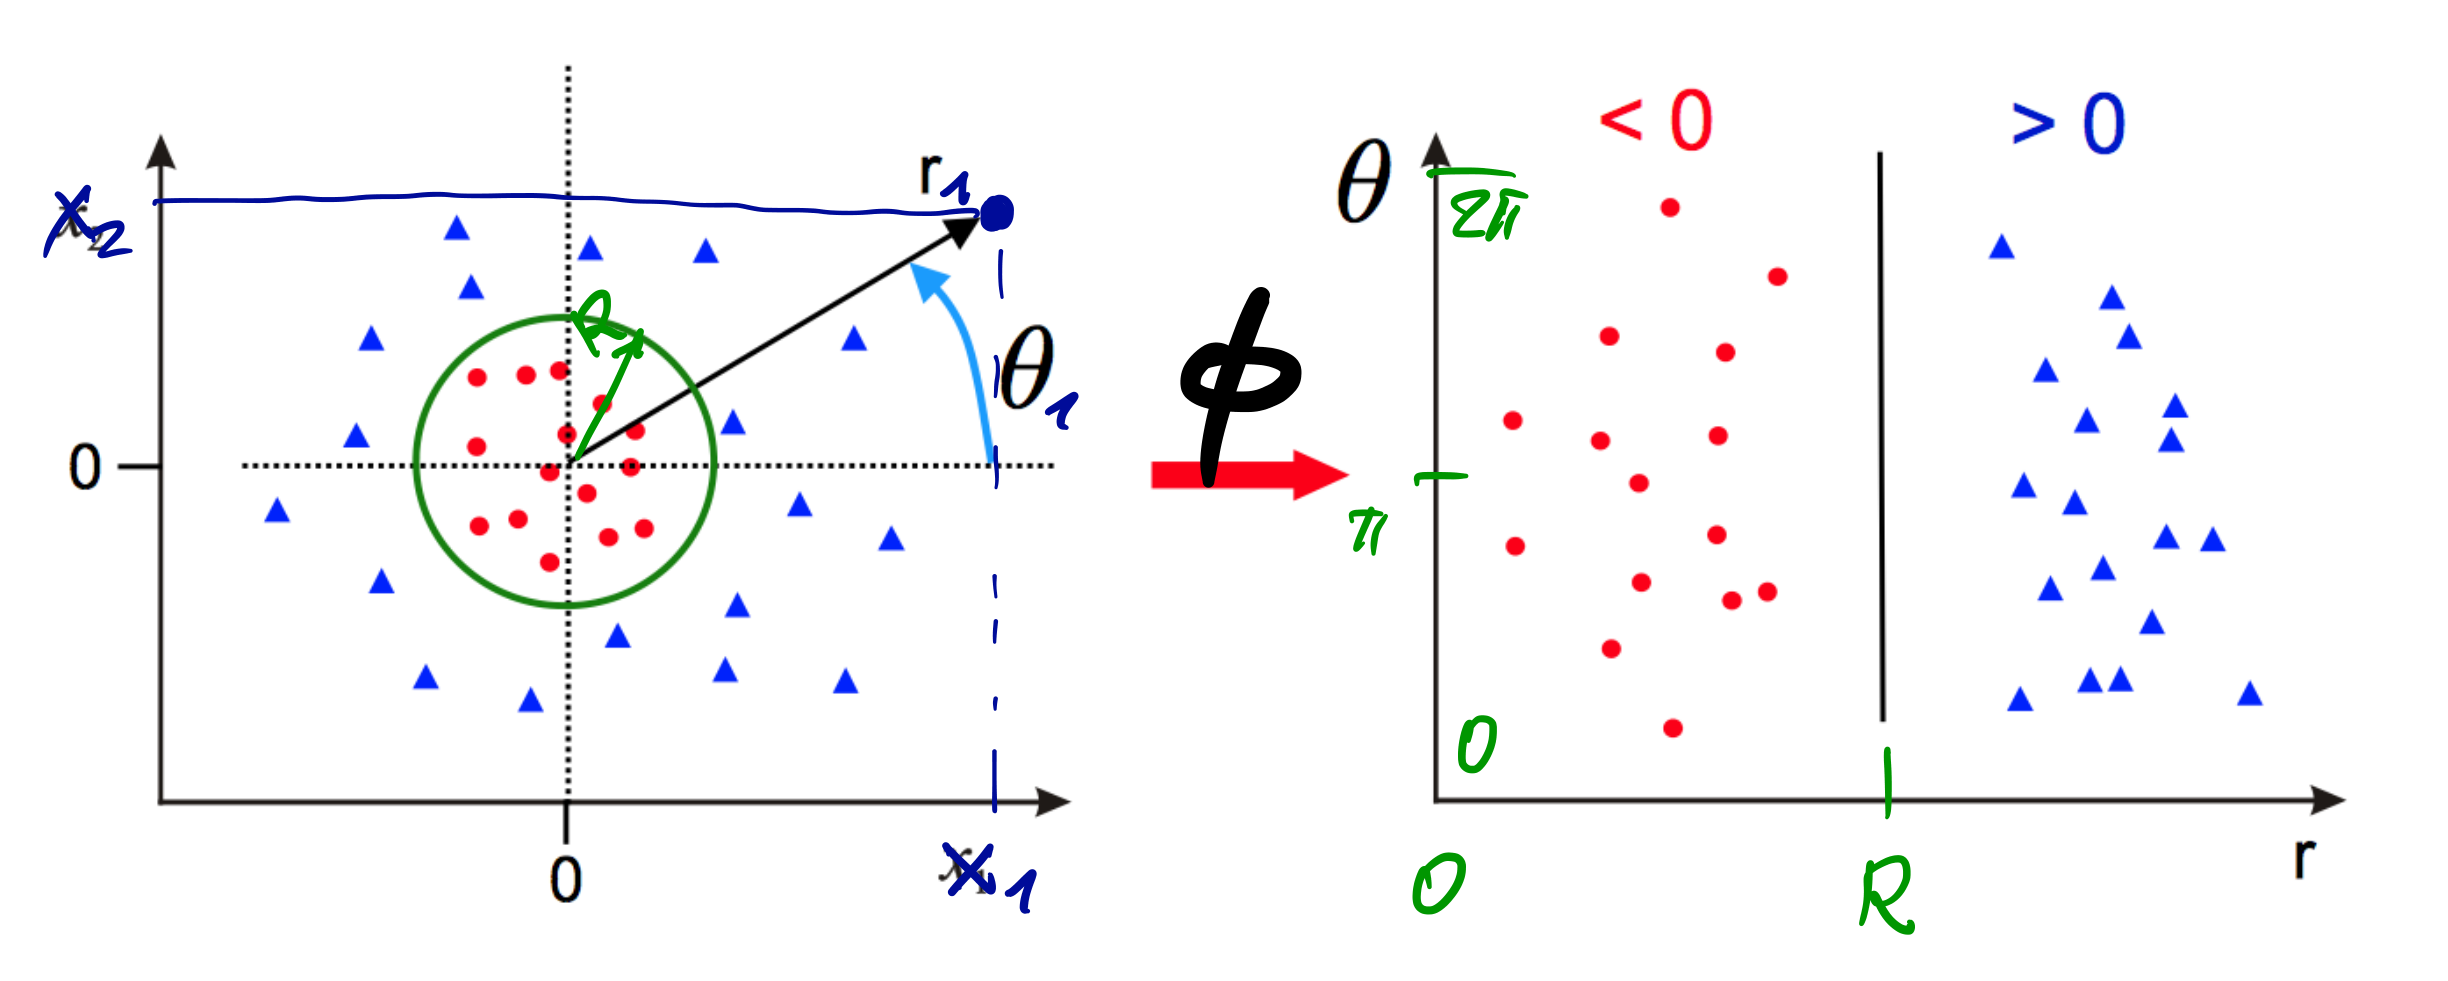
\includegraphics[keepaspectratio,width=0.7\linewidth]{Pictures/kernel_functions_polar_coordinates}
	\caption{Transformation from cartesian to polar coordinate system}
	\label{fig:kernelfunctionspolarcoordinates}
\end{figure}

\begin{figure}[htb!]
	\centering
	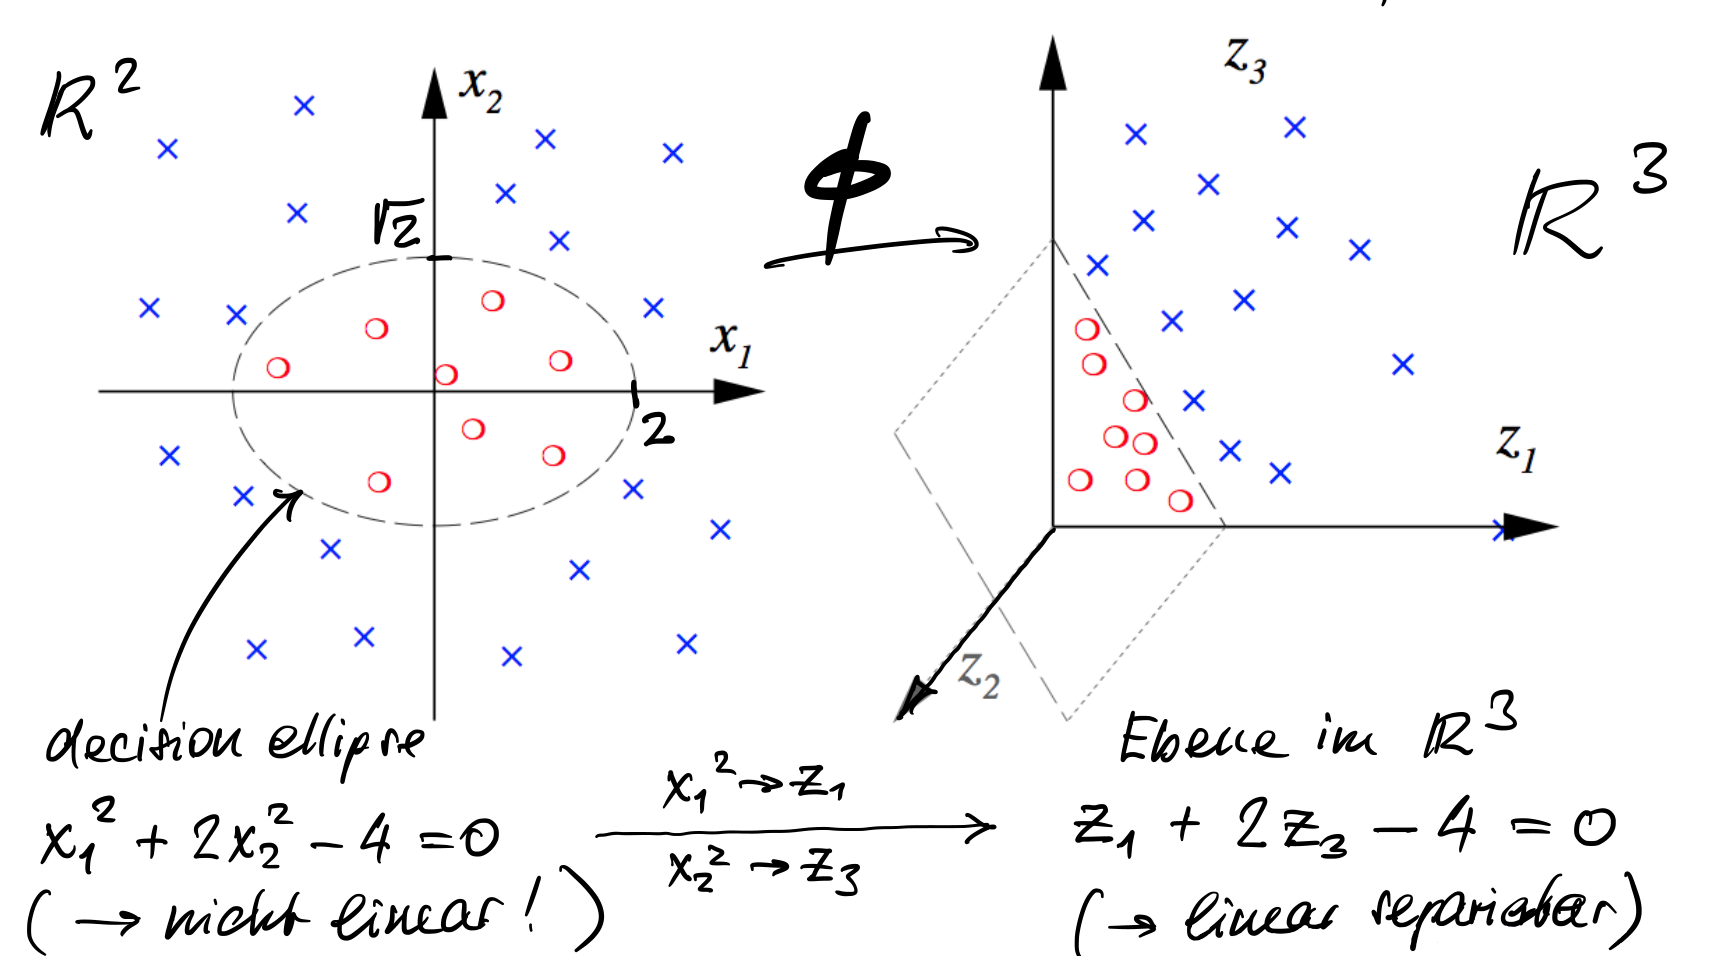
\includegraphics[keepaspectratio,width=0.7\linewidth]{Pictures/kernel_functions_polynomial_mapping}
	\caption{Transformation to higher dimension}
	\label{fig:kernelfunctionspolynomialmapping}
\end{figure}

Kernel function $\Phi$ satisfy:
\begin{enumerate}[leftmargin=*, labelindent=5cm, labelsep=0.5cm]
	\item[positive semidefinite]$\forall x_1,x_2(\Phi(x_1,x_2)\geq 0)$
	\item[symmetric] $\Phi(x_1,x_2) = \Phi(x_2,x_1)$
\end{enumerate}

\section{Clustering and Association Rules}

\subsection{k-Means Algorithm}

The k-Means algorithm is an algorithm that automatically identifies cluster centers. One has to specify the amount of clusters one wants before it can start though. The algorithm functions as follows:

\begin{enumerate}
	\item Input: Number of clusters $k>0$ and data points $x_1,...,x_n \in \mathbb{R}^m$
	\item Randomly choose $k$ cluster centers $\mu_1,...,\mu_k \in \mathbb{R}^m$
	\item Repeat until convergence
	\begin{enumerate}
		\item Assign each data point $x_i$ to its neares cluster center $\mu_j$
		\begin{equation*}
			c_i = \underset{j\in\{1,...,k\}}{\text{argmin}}\ \| x_i - \mu_j \|^2
		\end{equation*}
		\item  Update each cluster center to the mean of all assigned data points
		\begin{equation*}
			\mu_j := \frac{\sum_{i:c_i=j} x_i}{|\{i:c_i = j\}|}
		\end{equation*}
	\end{enumerate}
\end{enumerate}

\subsubsection{A note on the Euclidean Distance between two points}
\begin{align*}
	x &= (x_1,x_2)\\
	\| x \| &= \sqrt{x_1^2 + x_2^2}\\
	\| x \|^2 &= x_1^2 + x_2^2\\
	y &= (y_1, y_2)\\
	\| x - y \| &= \sqrt{(x_1 - y_1)^2 + (x_2 - y_2)^2}
\end{align*}

\subsubsection{Clustering Distortion}

The total distortion can be measured by summing up the squared distance between each point and it's cluster center
\begin{equation}
	\sum_{i=1}^{n}\| x_i -\mu_{c_i} \|^2
\end{equation}

The average distortion per data point is
\begin{equation}
	\frac{1}{n}\sum_{i=1}^{n}\| x_i -\mu_{c_i} \|^2
\end{equation}

Average distortion allows to compare clusterings over different data sets

\subsubsection{Convergence and Optimality}

Optimal clustering minimises the total distortion, which is a NP-hard problem for $x>1$. Therefore k-Means only approximates the optimal solution, but always converges, albeit not necessarily to a global minimum. In practice k-Means is executed several time and the clustering with minimum distortion is chosen.

\subsubsection{Choose the Number of Clusters}

The choice of clusters balances between low distortion and fewest number of clusters. The elbow method finds a good compromise in general (see figure \ref{fig:elbowmethod}).

\begin{figure}[htb!]
	\centering
	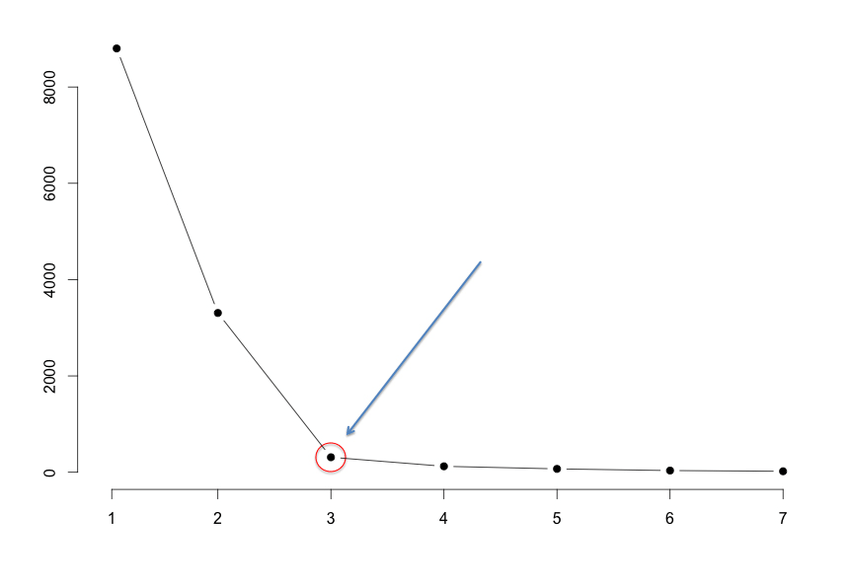
\includegraphics[keepaspectratio, width=0.4\linewidth]{Pictures/elbow_method}
	\caption{The elbow method to find the best number of clusters}
	\label{fig:elbowmethod}
\end{figure}

\subsection{Association}

An \textbf{association rule} is an implication $X\rightarrow Y$, where $X$ and $Y$ are disjoint item sets (refer to \ref{fig:associationrule}).

\begin{figure}[htb!]
	\centering
	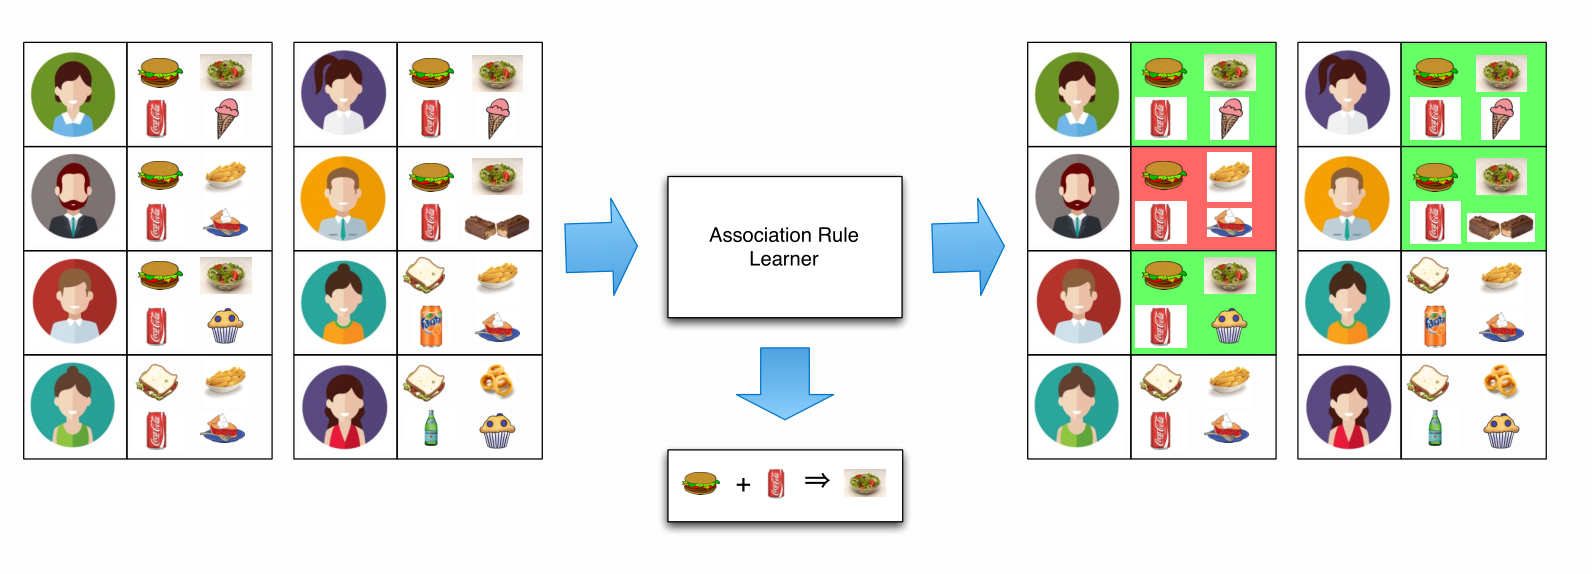
\includegraphics[keepaspectratio, width=0.7\linewidth]{Pictures/association_rule}
	\caption{A graphical representation of an Association Rule Learner}
	\label{fig:associationrule}
\end{figure}

\subsubsection{Support of a Set of Items}

Support is the proportion of transactions which contains a specific item set, and thus measures how frequently items ar bought together.
\begin{equation*}
	\text{support}(\{i_1,...,i_n\}) = \frac{\#\text{purchases of \{i_1,...,i_n\}}}{\# \text{transactions}}
\end{equation*}

\begin{figure}[htb!]
	\centering
	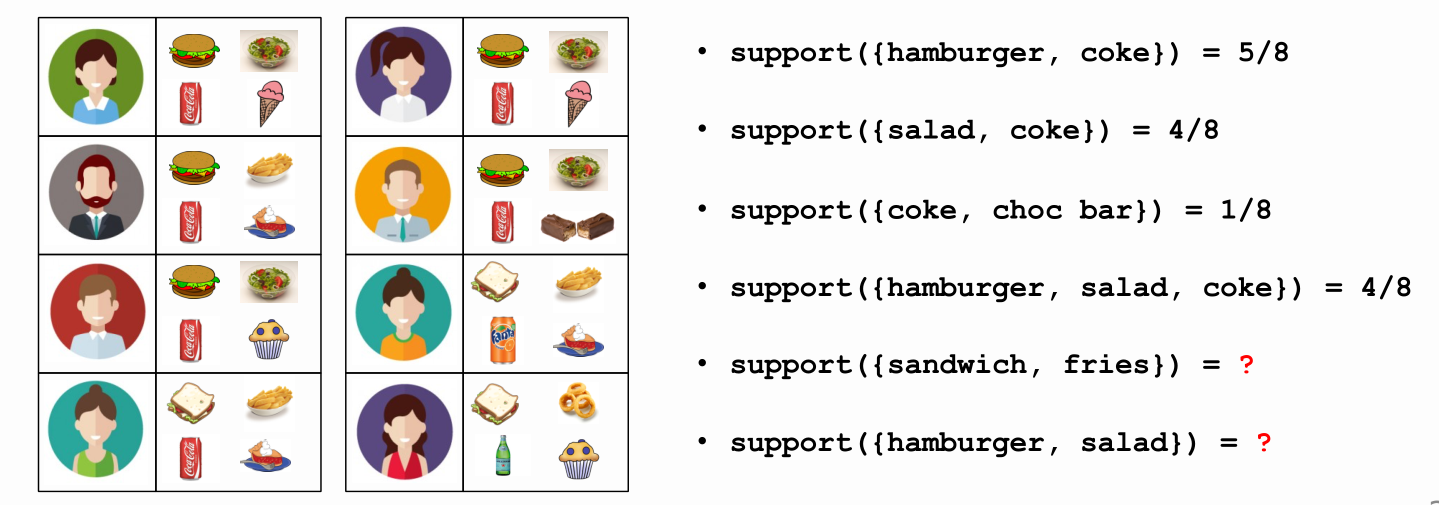
\includegraphics[width=0.7\linewidth, keepaspectratio]{Pictures/support_example}
	\caption{Examples of support}
	\label{fig:supportexample}
\end{figure}

\subsubsection{Support of an Association Rule}

The support of an association rule is defined as
\begin{equation*}
	\text{support}(X\rightarrow Y) = \text{support}(X\cup Y)
\end{equation*}

The support is \emph{direction invariant} and therefore cannot measure the quality of a directed rule
\begin{equation*}
	\text{support}(X\rightarrow Y) = \text{support}(Y\rightarrow X)
\end{equation*}

\begin{figure}[tbh!]
	\centering
	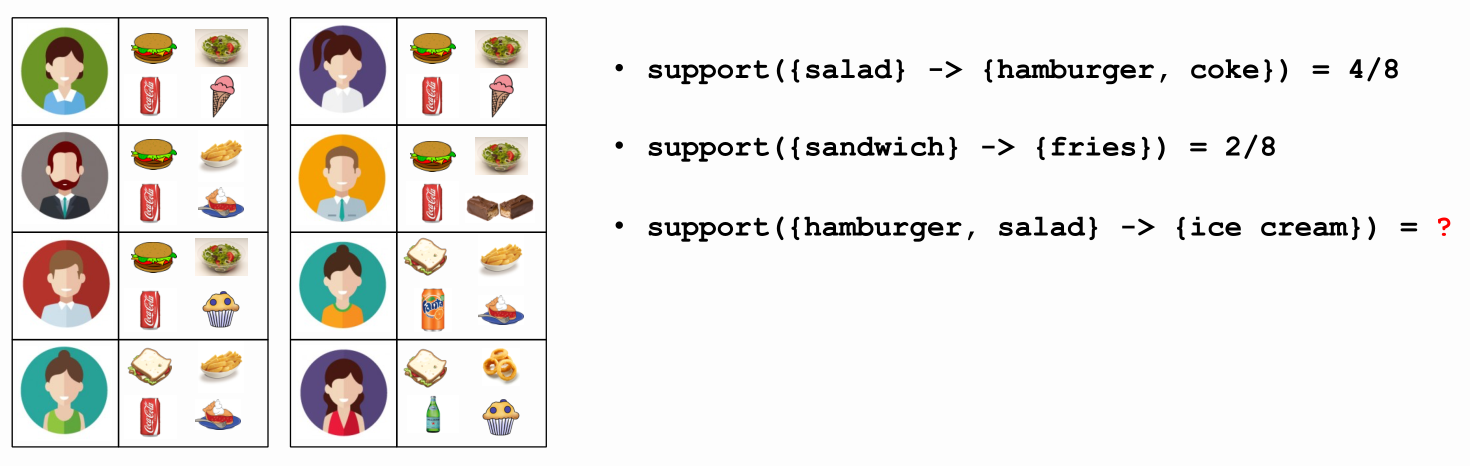
\includegraphics[width=0.7\linewidth, keepaspectratio]{Pictures/support_association_rule}
	\caption{Support of association rules}
	\label{fig:supportassociationrule}
\end{figure}

The support measures how frequently an item set occurs in the data. Rules with low support may occur simply by chance, while \textbf{good association rules have a high support}.

\begin{theorem}
	Support = Interestingness
\end{theorem}

\subsubsection{Confidence of an Association Rule}

The \textbf{confidence} of an association rule is defined as

\begin{equation*}
	\text{confidence}(X\rightarrow Y) = \frac{\text{support}(X\cup Y)}{\text{support}(X)}
\end{equation*}

\begin{figure}[tbh!]
	\centering
	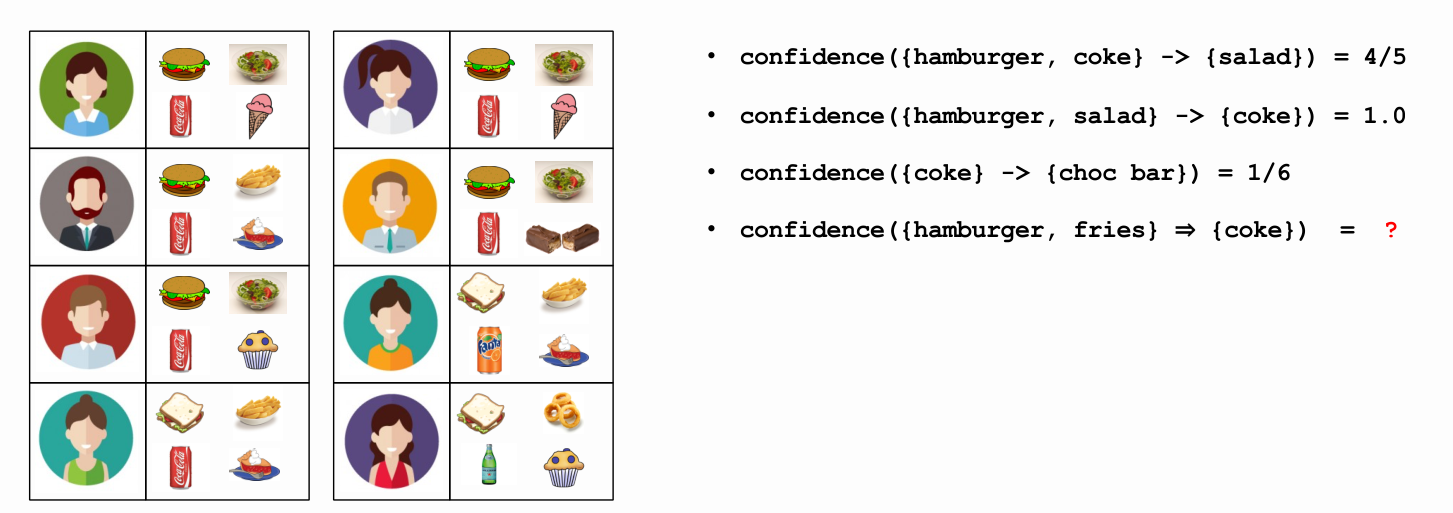
\includegraphics[width=0.7\linewidth, keepaspectratio]{Pictures/confidence_association_rule}
	\caption{Examples of confidence}
	\label{fig:confidenceassociationrule}
\end{figure}

For a given rule $X \rightarrow Y$, the higher the confidence, the more likely it is for $Y$ to be present in transactions that contain $X$. Confidence therefore measures reliability or trustworthiness of a rule, and a \textbf{good association rule has high confidence}.

\begin{theorem}
	Confidence = Trustworthiness
\end{theorem}

\subsubsection{Apriori Algorithm}

Given a set of transactions we want to find all rules having a minimum support $\geq \text{min}_s$ and a minimum confidence $\geq \text{min}_c$. The Apriori Algorithm finds such association rules in two steps:
\begin{enumerate}
	\item Generate frequent item sets satisfying the support threshold
	\item Extract rules from frequent item sets satisfying the confidence threshold
\end{enumerate}

The Apriori Algorithm has the following two properties, the second one allows for efficient pruning (refer to figure \ref{fig:supersetpruning}):

\begin{enumerate}
	\item If an item set is \textbf{frequent} (has high support), all of its subsets must be frequent too
	\item If an item set is \textbf{infrequent} (has low support), all of its super-sets must be infrequent too
\end{enumerate}

\begin{figure}[tbh!]
	\centering
	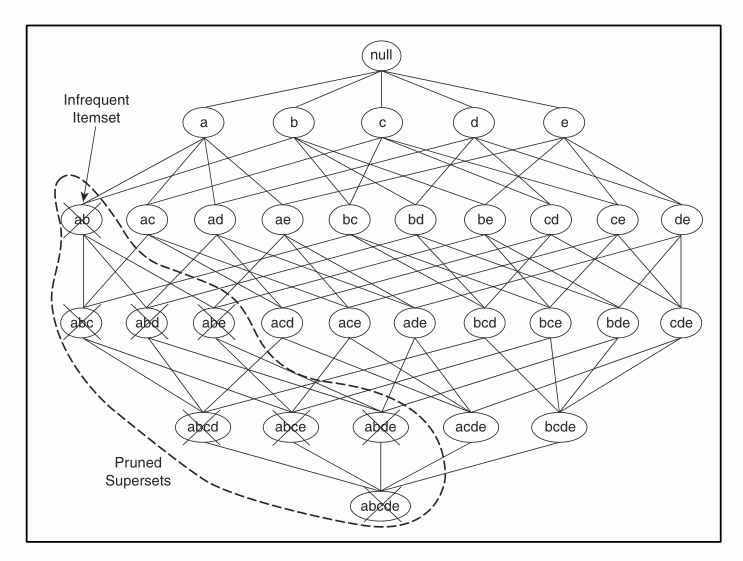
\includegraphics[width=0.5\linewidth, keepaspectratio]{Pictures/superset_pruning}
	\caption{Pruning of supersets of sets with low support}
	\label{fig:supersetpruning}
\end{figure}

After the pruning we generate Rules from the Frequent Item Sets and prune this tree as well. The method for pruning is based on the fact that if a rule $[X \rightarrow Y - X]$ violates the confidence threshold, then any rule $[X’ \rightarrow Y - X’]$ with $X’$ being a subset of $X$ violates the confidence threshold as well (refer to figure \ref{fig:subsetpruning})

\begin{figure}[tbh!]
	\centering
	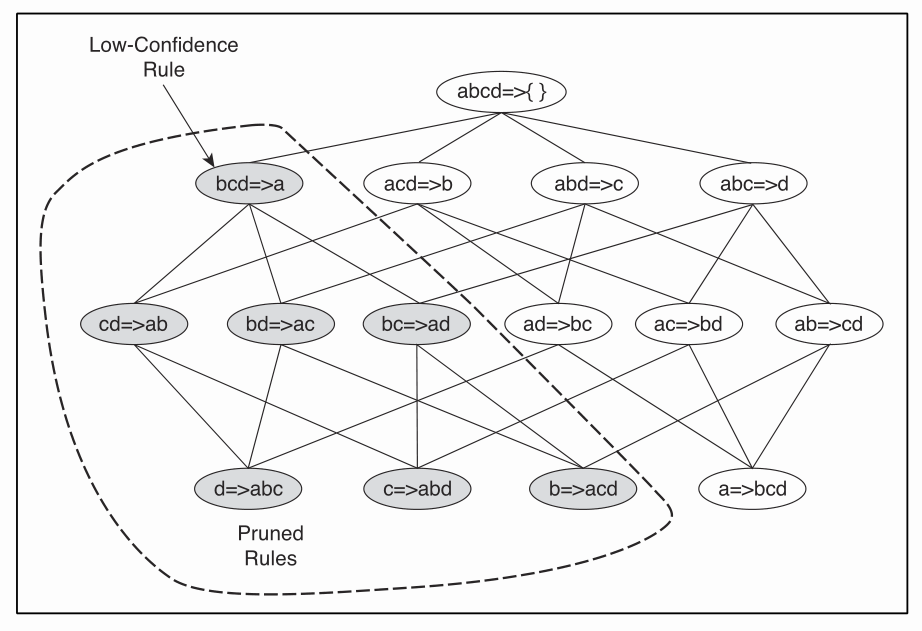
\includegraphics[width=0.7\linewidth, keepaspectratio]{Pictures/subset_pruning}
	\caption{Pruning of subset of a low confidence set}
	\label{fig:subsetpruning}
\end{figure}

\subsubsection{Lift of an Association Rule}

The \textbf{lift} of an association rule is defined as and measures how many times more often $X$ and $Y$ show up together than expected if they were statistically independent.

\begin{equation*}
	\text{lift}(X\rightarrow Y) = \frac{\text{support}(X\cup Y)}{\text{support}(X)\cdot\text{support}(Y)}
\end{equation*}

\begin{figure}[tbh!]
	\centering
	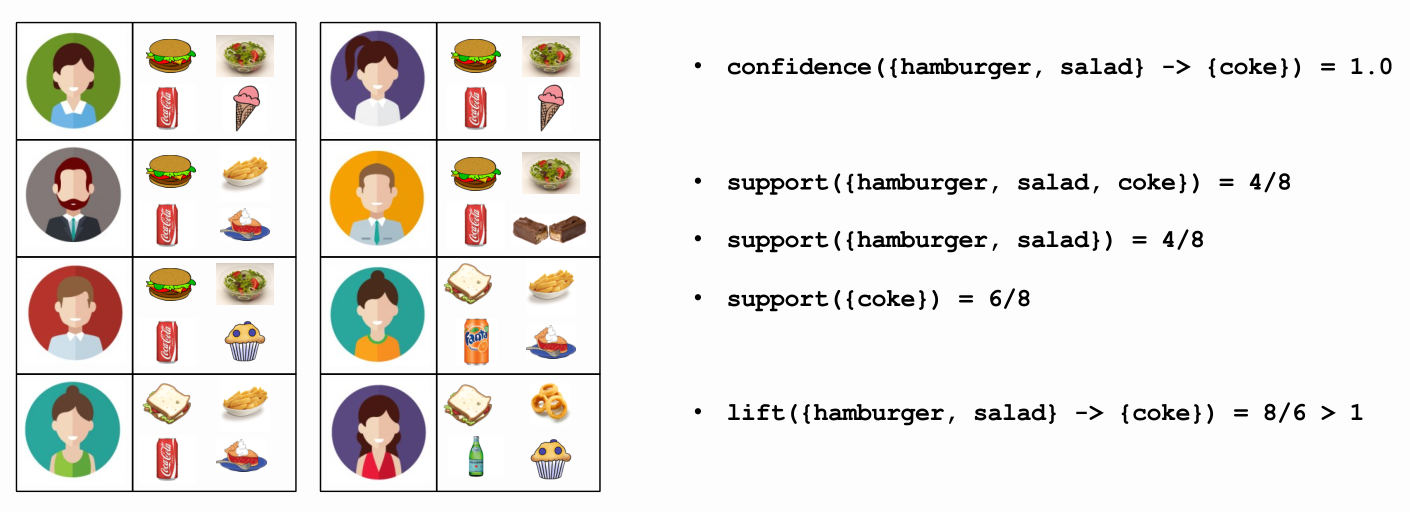
\includegraphics[width=0.7\linewidth, keepaspectratio]{Pictures/lift_association_rule}
	\caption{Example of lift}
	\label{fig:liftassociationrule}
\end{figure}

\begin{itemize}[leftmargin=*, labelindent=3cm, labelsep=1cm]
	\item[lift = 1] $X$ and $Y$ are statistically independent
	\item[lift < 1] indicates that $X$ and $Y$ appear less often together than expected, the occurrence of $X$ has a negative effect on the occurrence of $Y$ and vice-versa, $X$ and $Y$ are \textbf{anti-correlated}
	\item[lift > 1] indicates that $X$ and $Y$ appear more often together than expected, the occurrence of $X$ has a positive effect on the occurrence of $Y$ and vice-versa, $X$ and $Y$ are \textbf{correlated}
\end{itemize}

In general, the larger the lift value, the stronger the association between $X$ and $Y$. A good rule has high lift.

\begin{theorem}
	Lift = Association Strength
\end{theorem}

\section{Anomaly or Outlier Detection}

Anomaly or Outlier Detection is an important topic in unsupervised learning. Anomaly and outlier are used as synonyms. Anomalies are patterns in data that do not conform to a well-defined notion of normal behavior.

\begin{figure}[tbh!]
    \centering
    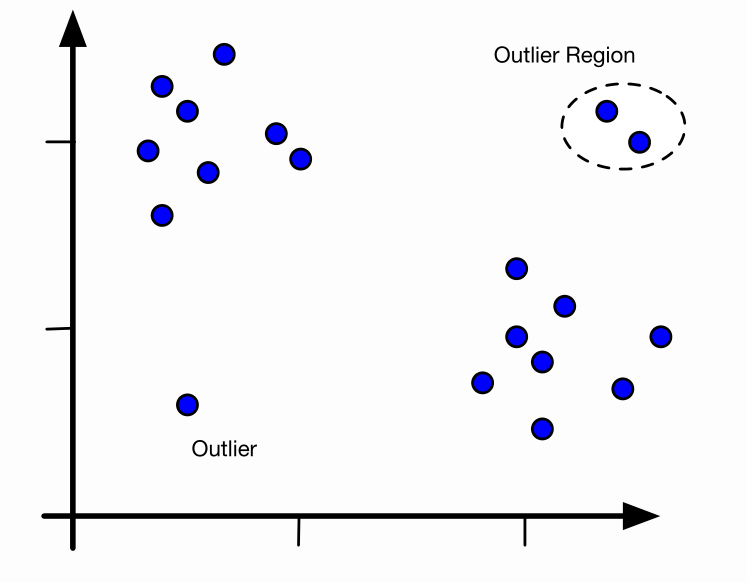
\includegraphics[width=0.4\linewidth, keepaspectratio]{Pictures/outlier_examples}
    \caption{Example of an outlier and outlier region}
    \label{fig:outlierexamples}
\end{figure}

We differentiate between three types of outliers

\begin{enumerate}
    \item \textbf{Global outliers} deviate significantly from the rest of the dataset
    \item \textbf{Contextual outliers} deviate significantly with respect to a specific context
    \item \textbf{Collective outliers} deviate as a group from the entire dataset but not necessarily as individuals
\end{enumerate}

We can solve the problem of outlier detection with machine learning:

\begin{itemize}[leftmargin=*, labelindent=5cm, labelsep=0.5cm]
    \item[\textbf{Supervised Learning}] Outlier detection can be considered a classification problem with categories \emph{normal} and \emph{outlier}.\\
        When outliers are rare events, collecting enough training data becomes a severe issue, and special measures must be taken because the two classes are extremely disbalanced
    \item[\textbf{Unsupervised Learning}] These methods assume that outliers deviate from the structural pattern of normal data objects.
    \begin{enumerate}
        \item Statistical Methods
        \item Proximity-based Methods
        \item Clustering Methods
    \end{enumerate}
\end{itemize}

\subsection{Statistical Methods}
Statistical methods assume that normal data objects are generated by a stochastic model, and that data not following that model are outliers.

\begin{enumerate}
    \item Assumption: The data follows a normal distribution with parameters $\mu$ and $\sigma^2$
    \item Method: Find best parameters with Maximum Likelihood method
    \item Conclusion: Find threshold were most of the data is located, for example $\mu \pm 3\sigma$ and classify all data outside of this range as outliers
\end{enumerate}

\begin{figure}[tbh!]
    \centering
    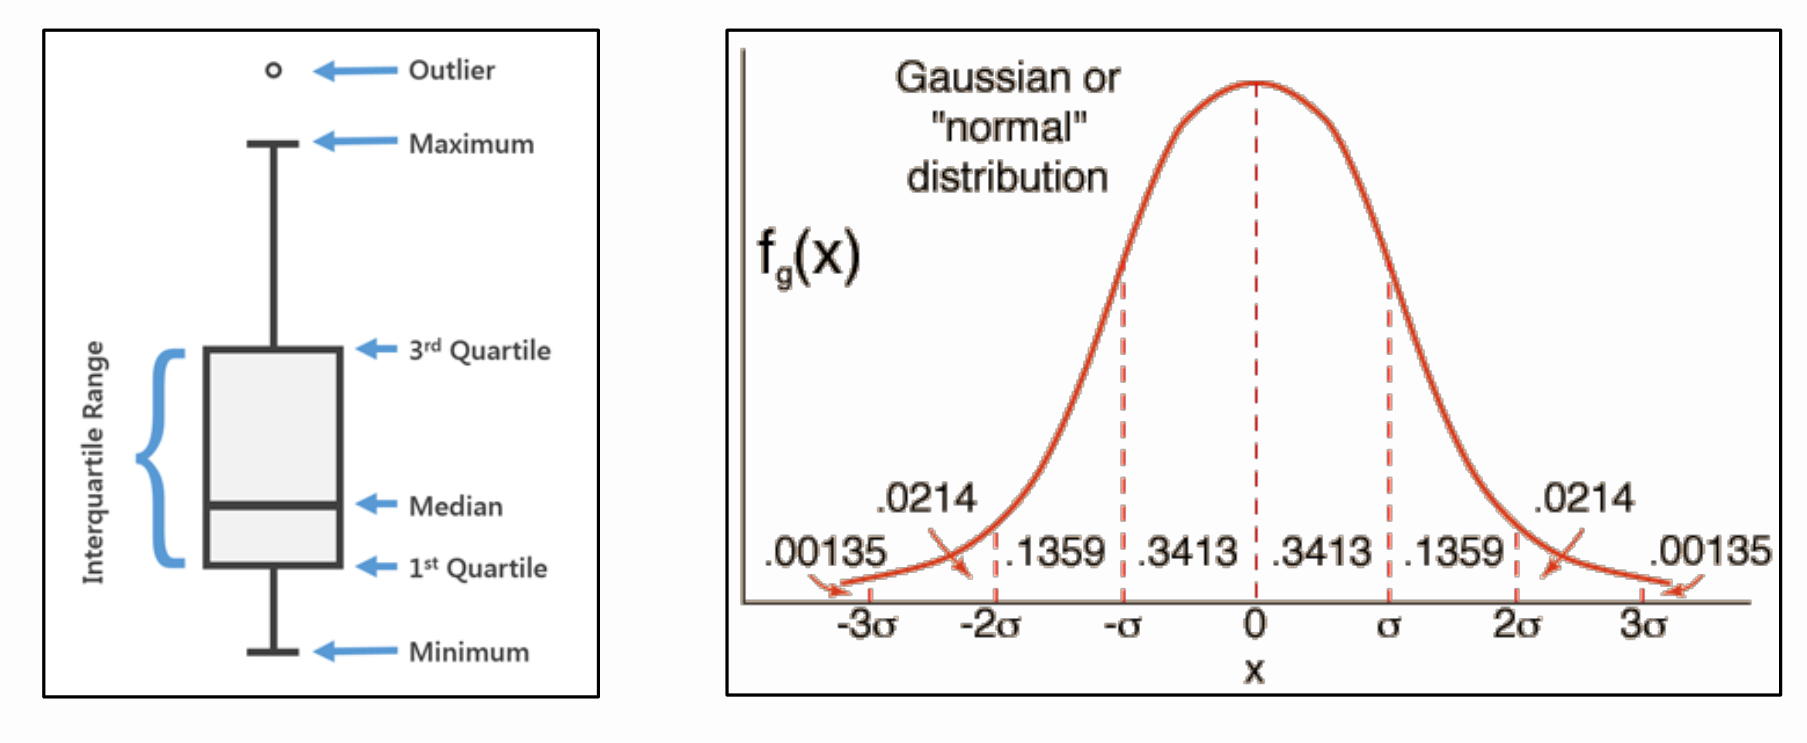
\includegraphics[width=0.8\linewidth, keepaspectratio]{Pictures/outlier_boxplot}
    \caption{Comparison of BoxPlots to Normal Distribution}
    \label{fig:outlierboxplot}
\end{figure}

Observe that this techniques for anomaly detection consider only single variables.
% TODO add multiple variable anomaly detection from exercises

\subsection{Proximity-based Methods}

In proximity-based methods, records that are far from others are considered outliers. There are two types of proximity-based methods:
\begin{enumerate}
    \item \textbf{Distance based methods} find outliers with respect to the global dataset
    \item \textbf{Density-based methods} find outliers with respect to local neighbourhood
\end{enumerate}

\begin{figure}[tbh!]
    \centering
    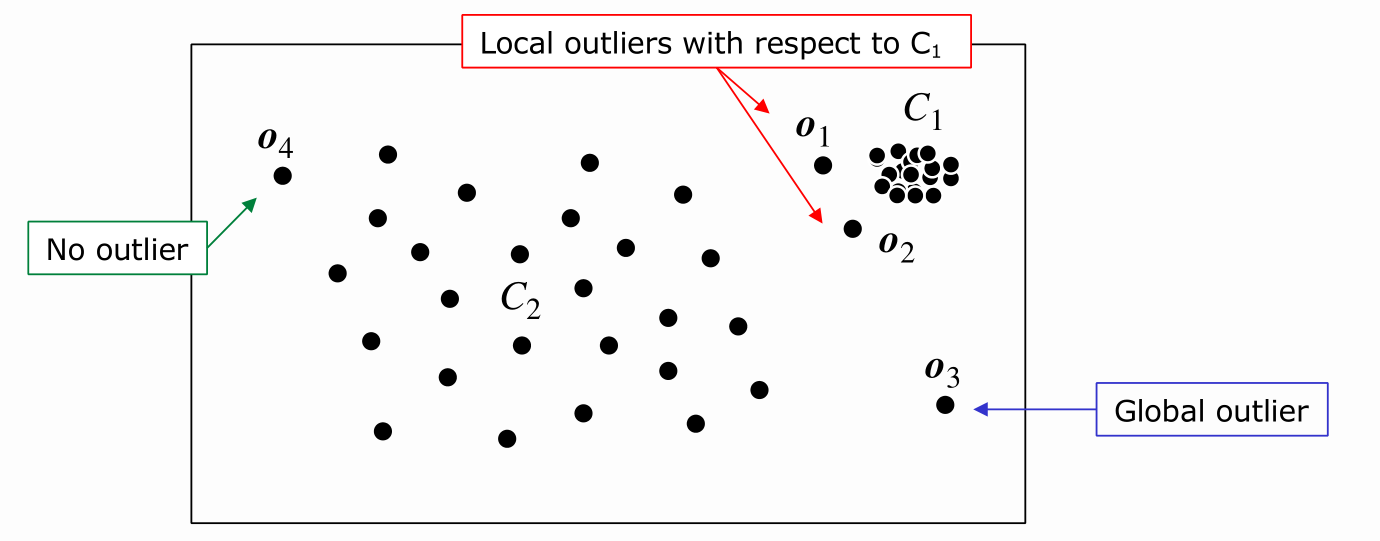
\includegraphics[width=0.6\linewidth, keepaspectratio]{Pictures/outlier_proximity-based}
    \caption{Outliers classified by proximity-based methods}
    \label{fig:outlierproximity-based}
\end{figure}

\subsubsection{Distance-Based Outliers}

\begin{itemize}
    \item Specify a distance threshold $r>0$ and a fraction threshold $0<\pi\leq 1$
    \item For each record count the numbers of other records in the $r$-neighbourhood
    \item Consider a record as outlier if $\frac{|\{o'\in D: o \neq o'\ \text{and}\ dist(o,o')\leq r \}|}{|D|} \leq\pi$
\end{itemize}

\subsubsection{Density-Based Outliers}

The density around a non-outlier is similar to the density around its neighbours, while the density around an outlier is significantly different from its neighbours (refer to figure \ref{fig:outlierdensity-based}).

\begin{figure}[tbh!]
    \centering
    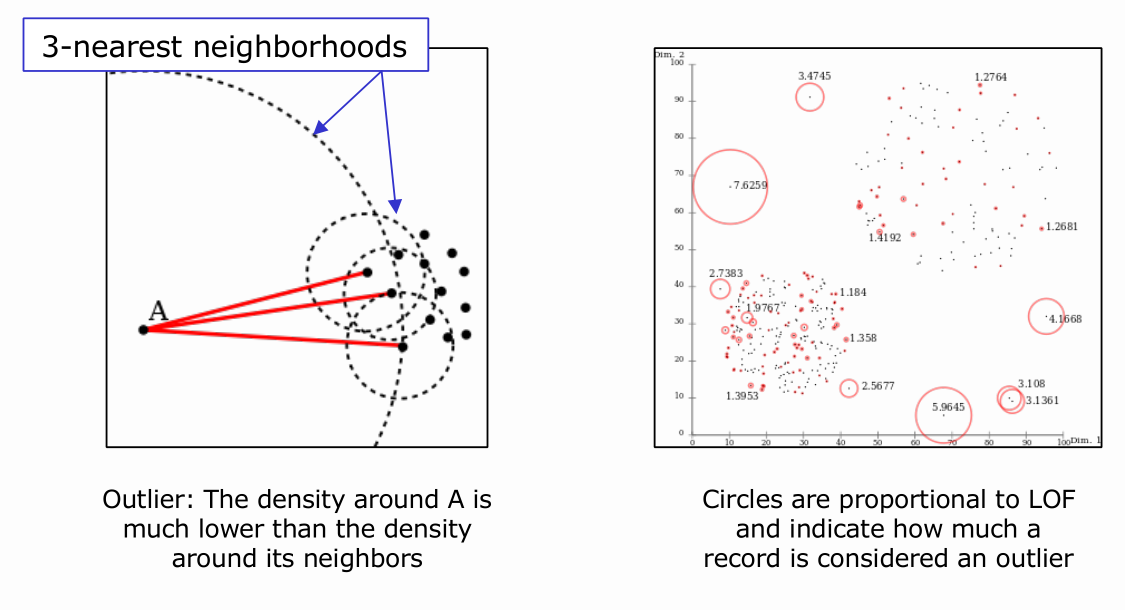
\includegraphics[width=0.6\linewidth, keepaspectratio]{Pictures/outlier_density-based}
    \caption{Graphical representation of density-based outlier detection}
    \label{fig:outlierdensity-based}
\end{figure}

The local outlier factor (LOF) is a score that indicates how likely it is that a certain data point is an outlier. A $\text{LOF} \approx 1$ means no outlier, while $\text{LOF} \gg 1$ means outlier. The k-Distance is the distance of a point to its k-th neighbour.

\paragraph{Reachability Distance}

The reachability distance is the maximum of the distance between two points and the k-distance of the second point. Consider it as a smoothing term, as a lower distance bound that depends on the neighbourhood density.

\begin{equation}
    \text{reachability distance}_k (A,B) = \text{max}\{\text{k-distance}(B), d(A,B) \}
\end{equation}

\begin{figure}[tbh!]
    \centering
    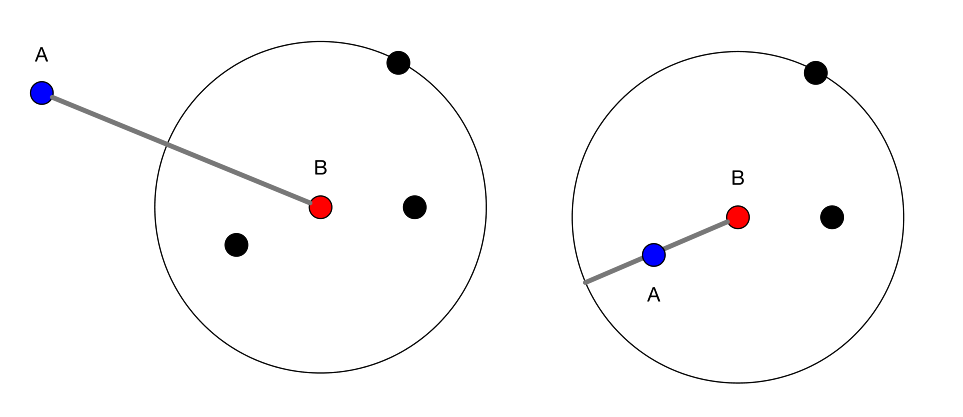
\includegraphics[width=0.5\linewidth, keepaspectratio]{Pictures/outlier_reachability_distance}
    \caption{Reachability distance visualised}
    \label{fig:outlierreachabilitydistance}
\end{figure}

\paragraph{Local Reachability Density (lrd)}

Calculate the reachability distance of $A$ to all its k-nearest neighbours and take the average of that number, then get the density by taking the inverse. Intuitively, the local reachability density tells how far we have to travel to reach the next point or cluster of points, the lower the local reachability density of a point, the less dense its region, the longer we have to travel.

\begin{equation}
    \text{lrd}_k (A) :=
    \frac{1}{
        \left(
        \frac{
            \sum_{B\in N_k (A)} \text{reachability distance}_k (A,B)
        }{|N_k(A)|}
        \right)
    }
\end{equation}

\begin{figure}[tbh!]
    \centering
    \includegraphics[width=0.5\linewidth, keepaspectratio]{Pictures/outlier_reachability_density}
    \caption{The local reachability density is not symmetric}
    \label{fig:outlierreachabilitydensity}
\end{figure}

\paragraph{Local Outlier Factor}

The local outlier factor is the local reachability density of a point in comparison to its k neighbours, more specifically, $k$ ratios of the local reachability distance of each point to its neighbouring points are calculated and averaged.

\begin{equation}
    \text{LOF}_k(A):= \frac{\sum_{B\in N_k (A)} \frac{\text{lrd}(B)}{\text{lrd}(A)}}{|N_k(A)|} = \frac{\frac{\sum_{B\in N_k (A)} \text{lrd}(B)}{|N_k(A)|}}{\text{lrd}(A)}
\end{equation}

\begin{itemize}[leftmargin=*, labelindent=2cm, labelsep=1cm]
    \item[$\text{LOF}(k) \approx 1$] similar density as neighbors : \textbf{Normal}
    \item[$\text{LOF}(k) < 1$] higher density than neighbors : \textbf{Inlier}
    \item[$\text{LOF}(k) > 1$]  lower density than neighbors : \textbf{Outlier}
\end{itemize}

\subsection{Clustering Methods}

Clustering-based approaches detect outliers by examining the relationship between records and clusters.

\begin{enumerate}
    \item Records not belonging to any cluster are outliers
    \item Records with a large distance to their closest cluster center are outliers
    \item All records in a small and sparse cluster are considered outliers
\end{enumerate}

\begin{figure}[tbh!]
    \centering
    \includegraphics[width=0.7\linewidth, keepaspectratio]{Pictures/outlier_clustering_method}
    \caption{Different kind of cluster outliers}
    \label{fig:outlierclusteringmethod}
\end{figure}

\paragraph{Classification-based Approaches}

Train a classifier, a Support Vector Machine for example, to distinguish normal data from anomalies and generate the decision boundary of the normal class. New objects outside the decision boundary are considered outliers

\begin{figure}[tbh!]
    \centering
    \includegraphics[width=0.7\linewidth, keepaspectratio]{Pictures/outlier_clustering_method_classification}
    \caption{Example of a classifier for outlier detection}
    \label{fig:outlierclusteringmethodclassification}
\end{figure}

\section{Recommender Systems}

\subsection{Definition}

\begin{quote}
    \blockquote[Burke, 2002]{A recommender system is any system that produces individualized recommendations as output or has the effect of guiding the user in a personalized way to interesting or useful objects in a large space of possible options}
\end{quote}

Or easier said:

\begin{quote}
    \blockquote[Jennach et. al., 2010]{A recommender system is a software application capable of suggesting interesting things to its users after learning their preferences over time}
\end{quote}

So basically recommender systems are the algorithms that show up under your amazon searches as 'customers who bought [xxx] also bought [yyy]'.

As opposed to Support or Lift, recommender systems are \textbf{individualized}.

\vspace{10px}

The goal of recommender systems is to give customers a better overview, to help them cope with the information overload problem (Amazon currently has over 20'000 results of 'Laptop Stand', but I only need one).

As a nice side effect, companies make more sales, because their customers can actually find what they're looking for.

\subsection{History}

The history of recommender systems can be split into three waves:

\begin{description}
    \item[1st wave (1991 - 2000)] \mbox{}\\
          5-star ratings
    \item[2nd wave (2001 - 2010)] \mbox{}\\
          Integration of personal web pages/facebook/myspace etc.
    \item[3rd wave (2011 - )] \mbox{} \\
          Smart technologies, big data, voice activated assistants
\end{description}

\begin{figure}[htb!]
    \centering
    \includegraphics[keepaspectratio=true,height=15\baselineskip]{recommender_system.png}
    \caption{Generic Picture of a Commercial Recommender System}
    \label{fig:recommender_systems}
\end{figure}


\subsection{Business Model}

\begin{itemize}
    \item Recommender Systems are only proviced as SaaS (Software as a Service), you only rent the system
    \item All data is managed by the vendors. The clients only get the recommendations produced by this data and can display them at their will
    \item Subscription prices for these systems are related to their success, usually clients pay a percentage of their revenue
    \item Due to the recent privacy-boom, some customers and clients do not want to provide all shopping data to these system-vendors. They'd rather have an in-house system.
    \item Having loads of data is hardly bad, the \textit{real} success in these systems lies in the configuration of the system and the evaluation of the data. This requires a deep understanding of the recommender algorithm
\end{itemize}

\subsection{Recommendations by Associations}

Most people think alike. People who buy cereal mostly also buy milk.

To calculate the percentage of buyers who bought $Y$ after buying $X$:

\begin{equation}
    \frac{X\ and\ Y}{X}
\end{equation}

This method is simple enough, but does not really work. A good example of why this won't work is Anchovies Paste and Banana. Basically everybody who buys Anchovies Paste also buys Banana. Does that mean they should be sold together as a package? No. Because these two products do not have anything in common. You could pair up basically every 'exotic' product with Banana according to this calculation. This is the case because \textit{Everybody needs bananas}. The fact that they also bought Anchovies Paste does not have anything to do with the fact that they needed bananas

\vspace{10px}

A better way to calculate basically the exact same thing, without having the Anchovies/Banana problem would be to check the percentage of buyers who bought the Anchovies Paste and also bought bananas and compare that number to the percentage of buyers who has not bought Anchovies Pate but bought bananas. That way, the popularity of bananas is of no consequences.

\begin{equation}
    \dfrac{\dfrac{X\ and\ Y}{X}}{\dfrac{¬X\ and\ Y}{¬X}}
\end{equation}

\vspace{10px}

Another important thing to check before making a recommendation: What does the buyer already have in their cart? Let's take the example of a fast food restaurant: I am ordering ice cream and get the recommendation that I might also like ketchup. While I \textit{do} like ketchup (although Mayonnaise, especially garlic one is still superior), I do not necessarily want it as a side to my ice cream.

Another example: If I buy ski boots, you could assume that I already own a pair of skis, so why would you recommend me to buy yet another pair of skis? Most people who bought skis and ski boots probably bought them at the same time.

\vspace{10px}

To summarize:

\begin{itemize}
    \item Recommendations by Associations are \textit{fast}. No data collection and evaluation necessa4ry
    \item Associations are \textit{context aware}. Only pairs of products that match together will be recommended together
    \item Associations can be specifically \textit{tailored} to certain businesses
    \item Associations look at \textit{shopping carts} instead of buyers and do not consider the customers personal preferences
\end{itemize}

\subsection{Context-Based Recommendations}

Instead of checking what customers actually bought, why not check and leverage what customers \textit{want} to buy?

Thanks to user ratings, wish lists, watchlists, viewed items etc, online vendors can create a very detailed shopping profile of their customers.

\begin{figure}[htb!]
    \centering
    \includegraphics[keepaspectratio=true, width=\linewidth]{context_based_recommendations.png}
    \caption{Context Based Recommendations}
    \label{fig:context_based_recommendations}
\end{figure}

\begin{figure}[htb!]
    \centering
    \includegraphics[keepaspectratio=true, width=0.9\textwidth]{item_similarity.png}
    \caption{Item Similarity}
    \label{fig:item_similarity}
\end{figure}

The idea of Context-Based Recommendations is to recommend the user similar products they have not rated/bought yet.

\begin{enumerate}
    \item Manually or automatically attribute your catalog data
    \item Collect as much user preferences as you can (e.g. by ratings, wish lists, item viewed etc.)
    \item Compute predictions for products labelled with $?$ based on item similarity (See Equation \ref{eq:sim} on page \pageref{eq:sim})
    \item Recommend products with high prediction value
\end{enumerate}

\begin{wrapfigure}[14]{R}{0.5\textwidth}
    \centering
    \includegraphics[keepaspectratio=true,height=10\baselineskip]{context_based_recommendations_v2.png}
    \caption{Context Based Recommendations with Neighbours}
    \label{fig:context_based_recommendations_2}
\end{wrapfigure}
Another approach of Context-Based Recommendations is to analyze similar products:

\vspace{10px}

Neighbors $N_j$ refer to the (at most) $N$ rated items most similar to item $j$, $N$ being a hyperparameter that can be tweaked for improved algorithm-performance
\noindent Select only rated items with similarity $> 0$ (choose less than $N$ if you cannot find enough candidates)

\vspace{50px}

\begin{figure}[htb!]
    \centering
    \includegraphics[keepaspectratio=true, width=0.9\textwidth]{context_based_recommendations_v3.png}
    \caption{Similarity between books}
    \label{fig:book_similarity}
\end{figure}

\begin{figure}[htb!]
    \centering
    \includegraphics[keepaspectratio=true, width=0.9\textwidth]{context_based_recommendations_v4.png}
    \caption{Example of N-Based Context-Based Recommendations}
    \label{fig:context_based_example}
\end{figure}

\restoregeometry

Advantages of Contex-Based Recommendations

\begin{itemize}
    \item A users profile is built only from their own ratings and recommendations can therefore be better explained
    \item New items can be recommended without having to be rated first
\end{itemize}

Disadvantages

\begin{itemize}
    \item The user will never find something unexpected they might like in their recommendations
    \item Do product attributes really reflect how users decide?
    \item What do you recommend new users?
\end{itemize}


\subsection{User-to-User Collaborative Filtering}

\begin{wrapfigure}[14]{R}{0.5\textwidth}
    \centering
    \includegraphics[keepaspectratio=true,height=10\baselineskip]{user_similarity.png}
    \caption{Context Based Recommendations with Neighbours}
    \label{fig:neighbours}
\end{wrapfigure}
This approach is similar to the similar products context based recommendations, but instead of similar products, it compares the customer to \textit{other similar customers}.

A set of users who liked the same items in the past, probably share the same preferences. Therefore, the user gets recommendations of products that many 'Neighbours' (similar users) liked, but the user has not purchased (yet).


There's a similar approach as to the Context-Based Recommendations, but there's no need for product attributes anymore. The formula to calculate how much user $u$ will wile product $j$ is also fairly similar.

\begin{figure}[htb!]
    \centering
    \includegraphics[keepaspectratio=true, width=\linewidth]{user_to_user_collaborative_filtering.png}
    \caption{User to User Collaborative Filtering}
    \label{fig:user_to_user_collaborative_filtering}
\end{figure}

\begin{figure}[htb!]
    \centering
    \includegraphics[keepaspectratio=true, width=0.9\textwidth]{user_to_user_collaborative_filtering_v2.png}
    \caption{Similarity between users}
    \label{fig:user_similarity}
\end{figure}

\newpage

\begin{figure}[htb!]
    \centering
    \includegraphics[keepaspectratio=true, width=0.9\textwidth]{user_to_user_collaborative_filtering_v3.png}
    \caption{Example of N-Based User to User Filtering Recommendations}
    \label{fig:context_based_example}
\end{figure}


\subsection{Item-to-Item Collaborative Filtering}

Because user proviles constantly change, pre-computation does not necessarily work. In contrast, for pairs fo items, similarity is stable and can be pre-computed.

The main difference is that we compare row vectors for neighbour search instead of column vectors.

\begin{figure}[htb!]
    \centering
    \includegraphics[keepaspectratio=true, width=\linewidth]{item_to_item_collaborative_filtering.png}
    \caption{Item to Item Collaborative Filtering}
    \label{fig:item_to_item_collaborative_filtering}
\end{figure}


Advantages of Collaborative Filtering Recommendations

\begin{itemize}
    \item Products from different categories can be recommended
\end{itemize}

Disadvantages

\begin{itemize}
    \item If the matrix is too sparsely filled, no neighbours will be found
    \item It needs loads of people to participate to make decent recommendations
    \item The system must first learn new users preferences
    \item Users with non-mainstream taste will not get decent recommendations
\end{itemize}

\vspace{10px}

To improve the recommendations for sparsely filled matrices, there's something called \textbf{Low Rank Matrix Factorization}. The matrix we saw before (Fig. \ref{fig:item_to_item_collaborative_filtering},
\ref{fig:user_similarity}, \ref{fig:book_similarity}) can be split up in two matrices, which are more densely filled.

One matrix holds all users and their ratings for the products they rated and the second matrix holds all products.


The first matrix (U) holds all users and their ratings. Each row is a user and all the ratings on all products they have made.

The second matrix (V) holds all the products and the rating they've gotten. This matrix is \textbf{transposed}.

\begin{figure}[htb!]
    \centering
    \includegraphics[keepaspectratio=true, width=\linewidth]{matrix_factorization.png}
    \caption{Low Rank Matrix Factorization}
    \label{fig:matrix_factorization}
\end{figure}

From this, we can see that the original matrix can be written as $U \times V^T$

\begin{minipage}{0.45\textwidth}
    \begin{align*}
        U =
        \begin{bmatrix}
            U_{1,1} & U_{1,2} & \hdots & U_{1,k} \\
            U_{2,1} & U_{2,2} & \hdots & U_{2,k} \\
            U_{3,1} & U_{1,2} & \hdots & U_{3,k} \\
            U_{4,1} & U_{4,2} & \hdots & U_{4,k} \\
            \hdots                               \\
            U_{n,1} & U_{n,2} & \hdots & U_{n,k} \\
        \end{bmatrix}
    \end{align*}
\end{minipage} \hfill
\begin{minipage}{0.45\textwidth}
    \begin{align*}
        V =
        \begin{bmatrix}
            V_{1,1} & V_{1,2} & V_{1,3} & V_{1,4} \hdots & V_{1,m} \\
            V_{2,1} & V_{2,2} & V_{2,3} & V_{2,4} \hdots & V_{2,m} \\
            \vdots                                                 \\
            V_{k,1} & V_{k,2} & V_{k,3} & V_{k,4} \hdots & V_{k,m} \\
        \end{bmatrix}
    \end{align*}
\end{minipage}

\vspace{10px}

$U_{1,1}$ is the rating User 1 gave the book 1,  $U_{2,1}$ is the rating User 2 gave the book 1 etc.

$v$ is the product matrix. The $V_1$ column stores all ratings book 1 has gotten, $V_2$ all ratings of book 2 etc.

\vspace{10px}

So if we want to check what rating user 3 has given book 4, we just need to calculate $U \times V^T$ and get the entry $(3,5)$.

That way, we can also 'guess' what rating a user would give a book they have not rated or bought yet. The rating of book 2 by user 2 is soterd in $U \times V, (2,2)$.


\subsection{Hybrid Recommender Systems}

The best result can usually be achieved if you mash multiple recommender-algorithms together. That way, their different advantages and disadvantages might cancel each other out. If you mix a content-based and a collaborative algorithm, you could for example eliminate the cold start problem.

But how could you interpret the different results from the different algorithms?

\begin{description}
    \item[Weighted: ] Score an item as a weighted sum of scores from different algorithms
    \item[Mixed: ] Results of different algorithms presented to the user
    \item[Cascade: ] One algorithm refines the result of another one
    \item[Switching: ] Different methods/algorithms can be used for different usecases
\end{description}

\subsection{Evaluation}

How would you evaluate recommender systems? Typical train/test/validate splits of your data will not work.

Instead the data must be split over several users, because to assess how good the recommendations are, we need the users whole shopping history.

\vspace{10px}

An often used performance measurement is $P@k$ (Precision @ k). How many of the $k$ recommended items were actually relevant. In case many users have less than $k$ recommended products, you could also go with $minP@k$.

\section{Dimensionality Reduction}

In Big Data, the provided data usually has \textit{a lot} of features, many of which do not add any significant information and could be deleted without losing anything important.

The following figure shows that more features don't necessarily produce better results

\begin{figure}[htb!]
    \centering
    \includegraphics[keepaspectratio, width=0.9\textwidth]{dimensionality_reduction.png}
\end{figure}

\vspace{10px}

\begin{wrapfigure}[20]{R}{0.4\textwidth}
	\centering
	\includegraphics[keepaspectratio,height=14\baselineskip]{data_points_2d}
\end{wrapfigure}

Let's say we want to reduce the dimensions on the right to one dimension instead of two. Which dimension should be removed to keep the most information? Price or Area?

\vspace{10px}

If you look at the following figure, you can see that for the correct solution, you need to think a bit outside the box. Instead of simply cutting away one or another dimension, the dimensions are \textit{rotated} and are a linear combination of the original dimensions. 

\vspace{-20px}

\begin{align*}
\text{Area} = \alpha_1 \cdot \text{Area} + \beta_1 \cdot \text{Price}
\end{align*}

\vspace{-30px}

\begin{align*}
\text{Price} = \alpha_2 \cdot \text{Area} + \beta_2 \cdot \text{Price}
\end{align*}

or more precisely:

\noindent\begin{minipage}{.5\linewidth}
\begin{align*}
x' = x \cdot cos \theta + y \cdot sin \theta
\end{align*}
\end{minipage}%
\noindent\begin{minipage}{.5\linewidth}
\begin{align*}
y' = -x \cdot sin \theta + y \cdot cos \theta
\end{align*}
\end{minipage}

\begin{figure}[htb!]
	\centering
    \includegraphics[keepaspectratio,width=\linewidth]{data_projections}
    \caption{Different ways to reduce dimensions of data points}
\end{figure}

\end{document}
